% document definition 
\documentclass[a4paper,11pt]{article} 

% create the following file in the input from the template
\newcommand{\PaperTitle} {Master Thesis Report}
\newcommand{\PaperSubject} {Multi Robot Motion Planning for Weld Quality Optimization}
\newcommand{\PaperTerm} {Summer/Winterterm 20xx}		
\newcommand{\PaperDate} {\today}			
\newcommand{\PaperLecturer} {Prof.Dr. Paul.G.Ploeger}	
\newcommand{\SecondAdvisor} {Prof. Dr. Rainer Bastert}	
\newcommand{\ThirdAdvisor} {Julian Diaz Posada}
\newcommand{\PaperLecturerEMail} {mailto:paul.ploeger@h-brs.de}
\newcommand{\SecondAdvisorEMail} {mailto:rainer.bastert@h-brs.de}
\newcommand{\ThirdAdvisorEMail} {mailto:julian.diaz@ipa.fraunhofer.de}
\newcommand{\Paperkeywords} {key1, key2, key3}			
\newcommand{\PaperMainWriter} {Poulastya Mukherjee}
\newcommand{\PaperMainWriterEMail} {mailto:poulastya.mukherjee@smail.inf.h-brs.de}

\usepackage[utf8]{inputenc} 
\usepackage{graphics}
\usepackage{url}
\usepackage{mya4page}
\usepackage{amsmath}
\usepackage{hyperref}
\usepackage{bibnames}
\usepackage{natbib}
\usepackage{path}
\usepackage{setspace}
\usepackage{epsfig}
%\usepackage{newunicodechar} 
%\DeclareUnicodeCharacter{FFFD}{?????}

%\usepackage{footmisc}
%\usepackage[perpage,symbol*]{footmisc} 

%---------------------------------------------------------------
\usepackage{color}
%% Hyperref setup
\usepackage{hyperref}
\hypersetup{
   pdftitle={ \PaperTitle },
   pdfsubject={ \PaperSubject },
   pdfauthor={ \PaperMainWriter <your.email@smail.inf.fh-bonn-rhein-sieg.de>},
   pdfkeywords={ \Paperkeywords },
   bookmarksopen=true,
   %citecolor=blue,
   %citebordercolor={0 0.4 0.7}
   colorlinks,
   citecolor=black,
   filecolor=black,
   linkcolor=black,
   urlcolor=black
}

\newcommand{\picHere}[3] { %
\begin{figure}[htp] %
\begin{center} %
\resizebox{!}{!}{\includegraphics{pictures/#1}} %
\caption{{\small#2}} %
\label{#3} %
\end{center} %
\end{figure} %
}

\newcommand{\picHereWidth}[4] { %
\begin{figure}[htp] %
\begin{center} %
\resizebox{!}{!}{\includegraphics[#4]{pictures/#1}} %
\caption{{\small#2}} %
\label{#3} %
\end{center} %
\end{figure} %
}

\newcommand{\picHereRes}[3] { %
\begin{figure}[htp] %
\begin{center} %
\resizebox{!}{!}{\includegraphics[totalheight=0.8\textheight]{pictures/#1}} %
\caption{#2} %
\label{#3} %
\end{center} % 
\end{figure} %
}

\usepackage{caption}
\usepackage{footmisc}
\usepackage{url}
\usepackage{enumitem}
\usepackage{anysize}
%\usepackage{adjustbox}
\usepackage{tikz}
\usepackage{amsmath}
\usepackage{algorithm}
\usepackage[utf8]{inputenc}
\usepackage{geometry}
\usepackage{subcaption}
\usepackage{graphicx}
%\usepackage{showframe} 
%\usepackage{algorithm2e}
\usepackage{algpseudocode}
\usepackage{booktabs}
\usepackage{hyperref}
\usepackage[utf8]{inputenc}
\usepackage{float}

\usepackage{xcolor}
%\usepackage{tabu}
%\usepackage{colortbl}
\usetikzlibrary{arrows,calc}
%\marginsize{2cm}{2cm}{0.5cm}{1cm}
\usepackage{makeidx}
\makeindex

\usepackage{titlesec}
\usepackage{afterpage}
\setcounter{secnumdepth}{4}

\titleformat{\paragraph}
{\normalfont\normalsize\bfseries}{\theparagraph}{1em}{}
\titlespacing*{\paragraph}
{0pt}{3.25ex plus 1ex minus .2ex}{1.5ex plus .2ex}
\usepackage[parfill]{parskip}
\usepackage{xcolor}

\newcommand{\MYhref}[3][blue]{\href{#2}{\color{#1}{#3}}}%
\makeatletter
\def\BState{\State\hskip-\ALG@thistlm}
\makeatother

\begin{document}
\singlespacing
% create title template 
\title{\PaperTitle\\\PaperSubject}
\author{\href{\PaperMainWriterEMail}{\PaperMainWriter \footnote{\href{\PaperMainWriterEMail} {poulastya.mukherjee@smail.inf.h-brs.de}} 
}\\%\vspace{0.5cm} \\ 
%Matrikel Nr.: 9019272 
\vspace{0.5cm} \\ 
B-IT Master Studies in Autonomous Systems \vspace{0.5cm} \\ 
Bonn-Rhein-Sieg University of Applied Sciences  \vspace{1.6cm}\\
Fraunhofer IPA \vspace{0.7cm} \\ \setcounter{footnote}{6}
Advisors: \href{\PaperLecturerEMail}{\PaperLecturer \footnote{\href{\PaperLecturerEMail} {Paul.Ploeger@h-brs.de}}}\\ %\small{\PaperTerm}}
\hspace{0.35cm}\href{\SecondAdvisorEMail}{\SecondAdvisor \footnote{\href{\SecondAdvisorEMail} {rainer.bastert@h-brs.de}}}\\
\hspace{0.35cm}\href{\ThirdAdvisorEMail}{\ThirdAdvisor \footnote{\href{\ThirdAdvisorEMail} {julian.diaz@ipa.fraunhofer.de}}}
}%\date{April 29, 2003}%\PaperDate}
\date{31 May,2017}
\maketitle

\onehalfspacing
\newpage
\clearpage
\section*{Declaration}

%\addcontentsline{toc}{chapter}{Declaration}
\renewcommand{\arraystretch}{0.4}

\vspace{20mm}

I, \textbf{Poulastya Mukherjee}, %Matrikel Nr.: 9025275, 
hereby declare that this work has not previously been submitted to this or any other university, and that unless otherwise stated, the content is entirely my own work.

%\singlespacing

\vspace{80mm}

\begin{table}[h]
 \begin{center}
  \begin{tabular}{ccc}
   
   \hspace{30mm}  & \hspace{30mm} &  \hspace{50mm} \\
   \cline{1-1}    \cline{3-3} \\
   Date           &  & Poulastya Mukherjee\\
  \end{tabular}
 \end{center}
\end{table}

\clearpage

%%% Local Variables: 
%%% mode: latex
%%% TeX-master: "../thesis"
%%% End: 

% crate abstract template 
\begin{abstract}


\end{abstract}

\newpage
\section{Acknowledgment}

I would like to express gratitude to both the supervisors, Prof. Paul G. Ploeger and Dr. Marek Schikora for their continuous guidance and invaluable inputs remarks and engagement through the learning process of this Research and Development project. Furthermore I would like to thank the entire team of Sensor Data Fusion (SDF) from Fraunhofer FKIE for their continued support and the help they provided whenever I faced any difficulty. Last but not the least I would like to thank all my dear friends in Masters in Autonomous Systems (MAS) for supporting me throughout the course of this project.
%\newpage
% document content begin here
%\input{background}
\newpage
\tableofcontents
\newpage
\listoffigures
\newpage
%\begin{theindex}
 
\end{theindex}

%\newpage
\section{Introduction}
\localtableofcontents
-----------------------
\subsection{Motivation}
Robotic Welding constitute majority of all robotic applications in industries today [1]. Large scale
industries with fixed manufacturing processes - like the car industry - traditionally uses MIG/MAG
welding operations in the car body workshops of the assembly lines. Due to falling costs of
robots and increasing precision and greater computational prowess, there is an increasing
number of smaller businesses, which follow client oriented manufacturing and produce unique
products designed specifically for each client- can now afford to use robotic manufacturing
processes to deliver highly customizable and precise goods.
Welding being one of the most common industrial process has been a subject of lot of ongoing
research for finding out the most suitable way to automate the task by using robots[1]. That
being said robotic welding is not at all a straightforward task because, it is difficult to
parameterize and to ensure weld quality assessment and control[1]. However robotic welding to
significant improvement both in terms of improvement in quality of product and reducing
manufacturing costs.
Along with the significant challenges mentioned above, robotic welding requires significant
knowledge both in the domain of the welding process - which skilled workers usually acquire
with years of experience - and programming the robot to perform the a welding task even on
simple workpieces[2]. A solution prevalent in the industry is the use of a teach pendant to guide
the robot’s manipulator for each task, in our case a weld seam, and then let it perform the task
autonomously[1,2,3]. The main disadvantage of this method is the significant longer teaching
time involved with each new workpiece. Thus the need of the hour is a simple programming
interface which will include the process knowledge of welding[1] and allow an operator to
generate programs for different weld seams without having to reprogram the robot. Even
though generating a welding program is quite simple, the complexity of the process increases
when several constraints are introduced - maintaining constant velocity during welding,
maintaining constant angle between tool tip and weld seam. The welding process can also be
affected by collision objects and presence of singular points in the path of the weld tool tip. While
avoiding collision is taken care of in the planning level, modern controllers are programmed to
handle singularities. However this kind of singularity avoidance usually results in deviation of the
behavior of the robot, which can result in poor quality weld surface.
An architecture- namely PPR (Product, Process and Robot) - has been proposed in [8] which uses
separate models for workpiece, robot and welding process and generates motion plans while
taking into account the process constraints. Due to the fact it uses sample based planning
algorithms, it can easily generate programs in new workspace environments as well as for new
3
workpieces with varying levels of complexity (linear edges, circular edges, discontinuous edges
etc).
\subsection{Overview}
\subsubsection{Objective}
The main objective of this work is to extend the existing RobotKit[8] software with multi-robot
planning capability. A 6 Dof manipulator will be the primary robot while a 2 dof rotary table will fulfill the role of second robot. Quite a number of multi robot approaches involving a
manipulator and a rotary table and two manipulators - already exists. Most notable among them
are Master/Slave[5] and non-Master/Slave approach[6], centralized[5] and decentralized
planning approach[6]. Our work will also evaluate the most suitable method among these based
on criterias like performance time and motion cost as mentioned in[1].
The second objective of the work is to improve the time of solution generated and reduce
solution cost, or in other words ensure greater compliance with existing manufacturing process
model[8].
The third objective of the work is to extend the existing State Validation model to include
Singularity and Reachability checking to generate more robust solution path.
\subsubsection{Proposed Contributions}
\begin{enumerate}
\item Extending the robot model of the PPR architecture from single robot welding process to
multiple robot welding approach .
\item Extending the state validation model of the PPR architecture to include singularity and
reachability check to ensure greater compliance with process model.
\item Improve performance of the planning algorithm by incorporating cost information and
replacing the randomized sampler with a sampler that samples based on the cost
information.
\item Evaluation of the proposed methods based on the performance changes in time of
generating solution and final solution cost.
\item Implementing other types of planning algorithms e.g. Multi query planners such as PRM
(Probabilistic Roadmap), SPArse Roadmap Spanner algorithm (SPARS), and other Single
query planners such as Rapidly-exploring Random Trees (RRT), Expansive Space Trees
(EST) and evaluating the performance with respect to the current problem in hand and
determining the best suited planning algorithm.
\item Evaluation of performance of the proposed changes of this work compared to existing
system based on time required to generate an optimal solution and cost of final solution.
\end{enumerate}
\subsection{Structure}
\begin{itemize}
 \item Chapter 2 describes the state of the art work in the fields of robotic path planning, multi robot path planning, robotic welding and optimizing weld planning.
 \item Section 3 describes the formulated problem and the plausible approach to solve it.
 \item Section 4 describes the approach taken to solve the initial position optimization of the table.
 \item Section 5 describes the experimental setup and the results of the experiment.
 \item Section 6 describes a use case in which the algorithm was implemented and subsequent results visualized.
 \end{itemize}







\newpage
 \section{Literature Review and State of the Art Analysis}

This chapter discusses the fundamentals of motion planning and related concepts. According to \cite{1} Motion planning consists of the following basic concepts which are prevalent irrespective of the type of planning problem:
\begin{itemize}
\item A \textbf{state space} definition in which the all probable scenarios related to the planning problem can be expressed
\item Modeling \textbf{time} respective to the problem, which can determine the speed of the execution of the problem or the order of sequence in which certain actions should be completed.
\item \textbf{Actions} are generated by plans which manipulate a state. The relationship between an an action and state change is generally described by the user. 
\item \textbf{Initial and Goal States} are the defined by the user. Actions are generated in order to convert the initial state to goal state.
\item Usually a \textbf{criterion} is specified in order to execute the actions to have a desired outcome. The two main goals of specifying a criterion are:
\begin{enumerate}
\item \textbf{Feasibility} The goal state can be reached 
\item \textbf{Optimality} Optimizes the performance of the planner e.g. reducing the planning time, taking actions with low cost, while achieving the goal state 
\end{enumerate}
\item \textbf{Plan} is generally a sequence of actions which might be simple or complex depending on the above mentioned criteria. 
\end{itemize}
In the following sections we delve deeper into motion planning for a manipulator 


\subsection{Motion Planning for Industrial Manipulators}
Motion planning is one of the most important aspects, when it comes to efficient program generation for industrial robots. Efficient motion planning can not only reduce time of task execution but also increase the rate of task completion by ensuring pitfalls of collision or singular points are avoided. For industrial manipulators generated plans need to be highly accurate and precise, hence large factories, namely automobile manufacturers employ robots which are pre programmed. However when it comes to small and medium enterprises, where the key goal is to adapt the manufacturing process based on the task at hand, hard coding a robot is not desirable. A very good example of this is welding, where the task changes based on the workpiece to be welded. Workpieces can be of varying complex geometrical structures and the multiple joints may need to welded at each iteration. Hence to maintain the same level of efficiency and speed of execution it becomes necessary to generate optimal motion plans.  

\subsubsection{Motion Planning for multi-DoF manipulators}

This section will highlight various existing motion planning approaches and discuss the pros and cons of each. In \cite{2}(Collision free path planning..) the authors model the state space as a 3D discretized grid in Cartesian coordinate system. The workpiece and fixtures are modeled as collision onjects. A heuristic is introduced which determines the distance between goal and current location while the collision avoidance is handled by a function which calculates the distance between current location and nearest collision objects and assigns a cost value based on the distance,as illustrated with equations \eqref{eq1},\eqref{eq2},\eqref{eq3}
\begin{equation}
\label{eq1}
obs = \sum x_{n} - m:x_{n} + m,y_{n} - m:y_{n} + m:z_{n} - m:z_{n} + m
\end{equation}
\begin{equation}
\label{eq2}
d = \sqrt{(x_{n} - x_{c})^2 + (y_{n} - y_{c})^2 + (z_{n} - z_{c})^2} + k*obs
\end{equation}
\begin{equation}
\label{eq3}
h = \sqrt{(x_{g} - x_{n})^2 + (y_{g} - y_{n})^2 + (z_{g} - z_{n})^2} + d
\end{equation}
here k is a constant [$x_{c},y_{c},z_{c}$] defines the current node, [$x_{n},y_{n},z_{n}$] represents the neighboring node and [$x_{g},y_{g},z_{g}$] defines the goal node. The A* algorithm is used to search the tree generated from this definition. Once a path to the goal state has been found, it is checked for inverse kinematic feasibility. The generated joint values are again checked for collision avoidance and then it is passed to the robot program. The main drawback of this approach is as the search tree tries to generate path which are away from obstacles while the workpiece object is designated as a collision object, which results in the manipulator moving far away from the workpiece after it has finished welding one edge. In cases where only one edge needs to be welded there the result will remain unaffected, however for multi edge welding this approach will lead to unnecessary large path costs. Another highlight of this approach was to reduce time of execution by generating trajectories, but the fact that each time the inverse kinematic values are generated; it is rechecked for collision leads to a delay (as collision checking is a computationally expensive process) and eliminates the gains of the trajectory planning. The fact that the authors did not publish any experimental evaluation of their method in the paper leaves open questions in this regard. \\
In \cite{3}(Online minimum time trajectory planning), the authors propose an algorithm for computing the trajectory of a 6 DoF manipulator which is explained with the help of the following flowchart. The equation \eqref{eq4} for calculating the maximum allowable acceleration and deceleration is 
\begin{equation}
\label{eq4}
\ddot{p}_{max} = \lambda_{min}u_{\ddot{p}}\in \Re^{m}
\end{equation}
where p is the maximum acceleration in cartesian space.

\begin{figure}[htbp] %  figure placement: here, top, bottom, or page
 \centering
   %\includegraphics[angle=90,width=10cm]{images/tbox.jpg}
   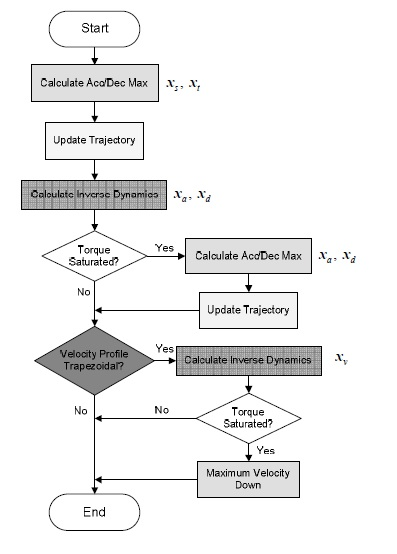
\includegraphics[width=9cm]{images/AlgoFlowchart.jpg}
   \caption[Trajectory Algorithm]
   {Trajectory Algorithm \footnotemark[\value{footnote}]}
   
\label{fig:img1}
\end{figure}

In \cite{4}(Integrated Time Optimal Trajectory Planning), the authors propose an algorithm to ensure compliance of the robot motion path and the planned path at high speeds. The authors demonstrate the working of their algorithm using a parameterized circular path using the equation \eqref{eq5}
\begin{equation}
\label{eq5}
q= \begin{bmatrix} q_{1}^{*}(t)\\ q_{2}^{*}(t)\\ q_{3}^{*}(t) \end{bmatrix} = \phi (\theta)|_{\theta=\theta^{*}(t)} = \begin{bmatrix} \phi_{1}(\theta)\\ \phi_{2}(\theta)\\ \phi_{3}(\theta) \end{bmatrix}|_{\theta=\theta^{*}(t)}
\end{equation}
In this equation the time parameterization is replaced by [$\theta$] parameterization which results in a synchronization of joints. Due to this joint velocities can be assigned with the following equation \eqref{eq6} for any velocity profile
\begin{equation}
\label{eq6}
q=\phi^{'}(\theta)\dot{\theta}
\end{equation}
After finding the optimal joint velocities, the joint angles are checked whether they satisfy the dynamic constraints. The authors then implemented an Proportional Derivative(PD) control feedback loop as a supplement to the motion planner. The authors propose their own controller apart from the already implemented PD controller and showed that their implementation lead to faster convergence to desired trajectory. The key takeaway from this paper is the parameterized model of trajectory planning which ensures the joint values can be assigned with variables dependent on angle value- [$\theta$] instead of time. 
\subsubsection{Motion Planning for manipulator and rotary table systems}
A key requirement for producing highest quality weld is the \textbf{downhand} welding position, in which the tangent line to the weld is horizontal and the normal vector to the weld is vertical \cite{5}(Manufacturing Process Planning for Robotic Arc-Welding Station). Due to this fixed criteria, planned paths for welding often end up having singular points in them, or they encounter collision objects which are difficult to avoid without violating the \textbf{downhand} welding position. One of the approaches taken in this regard is to include a till-roll workpiece manipulator or rotary table. In this paper \cite{5} the authors propose a cluster level operation planning with the optimization objective being - minimization of manufacturing time. \\
The authors divide the welding task into several clusters using a technique called weld seam clustering which arranges the welds into groups that do not require altering positioner configuration. The idea is to find the most optimum path through these clusters. The authors use a generalized TSP (GTSP) algorithm with GI3 heuristics which incorporates the following 3 phases (i) Generalized Initialization, (ii) Generalized Insertion , and (iii) Generalized Improvement. The above mentioned method was able to generate valid optimized solutions for 70-80$\%$ cases with a maximum optimization of 2.6$\%$. A possible reason for this method not generating valid solutions 100$\%$ of the time is due to the fact that, generated solutions are not subjected to kinematic constraints and only to the abstract space constraints like collision avoidance and seam selection checking.
In \cite{13}(Kinematic and dynamic analysis of 3 dof..) the authors describe a decentralized multi robot planning approach for general industrial tasks like welding, milling etc. with a 6 dof manipulator and a 3 dof rotary table. The dynamic equation is illustrated in \eqref{eq11}
\begin{equation}
\label{eq11}
M_{OK} = P_{i}(H_{OK}),H_{OK} = J_{OK}\omega_{i - OK}
\end{equation}
\eqref{eq11} is applied to every point, where each point shown with k symbol has $M_{OK}$ is the external torque, $H_{OK}$ is the rotational momentum and $J_{OK}$ is the moment of inertia for point k and $\omega_{i - OK}$ is the rotational velocity. 

\newpage
\subsection{Robotic Welding Processes}
In a recent study conducted by the American Welding Association revealed that the current demand for manufacturing welded goods are from small or medium batch manufacturing. In these settings robotic welding provides the most cost effective solution compared to human welders or hard automated setups. In this section we will discuss the various welding methodologies that are compatible with robotic welding and describe them briefly.\\
In \cite{6}(Welding Robots: Technology, System Issues and Application, Pires, J.N. and Loureiro,
A. and Bolmsjo, G), the authors state that the most prevalent method of welding in industry is the arc welding method. The two main types of arc welding are gas shielded tungsten arc welding (GTAW) and the gas shielded metal arc welding (GMAW). Apart from these, the various other methods of welding include Laser Beam Welding(LBW),Resistance Spot Welding (RSW), Friction Stir Welding (FSW).
Since GTAW and GMAW are the welding methods used for robotic welding in industries, we will elaborate on these.
\begin{itemize}
\item \textit{GTAW}: In this process an arc is created between a non-consumable electrode and the work metal which is then shielded by an inert gas to remove any atmospheric contamination. A current of 50-700 A is used to melt and fuse the work metal.
\item \textit{GMAW}: In this process a consumable electrode is used. A high current is applied which melts both the electrode and the work metal and fuses them together. An inert gas is used here as well to prevent contamination. The magnitude of current and voltage, size of electrode and type of inert gas used, determines the type of welding method:spray, short-circuiting, globular and pulsed transfer.
\end{itemize}

\subsubsection{Analysis of existing methods of Robtic Welding}
\textbf{Gas Tungsten Arc Welding (GTAW):}
\begin{figure}[htbp] %  figure placement: here, top, bottom, or page
 \centering
   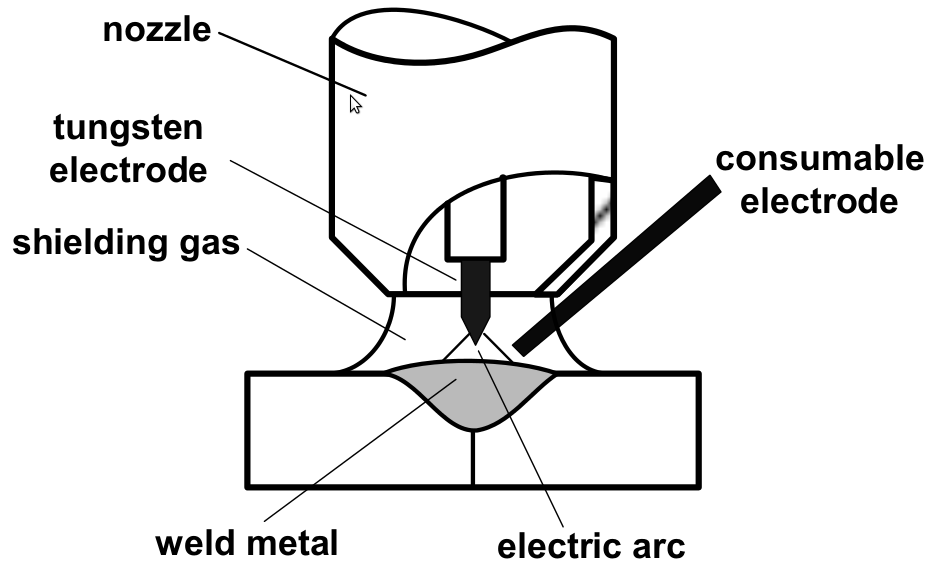
\includegraphics[width=9cm]{images/GTAW.png}
   \caption[Gas Tungsten Arc Welding]
   {Gas Tungsten Arc Welding \footnotemark[\value{footnote}]}  
\label{fig:img2}
\end{figure}
\newpage
\textbf{Gas shielded metal arc welding (GMAW):}

\begin{figure}[htbp] %  figure placement: here, top, bottom, or page
 \centering
   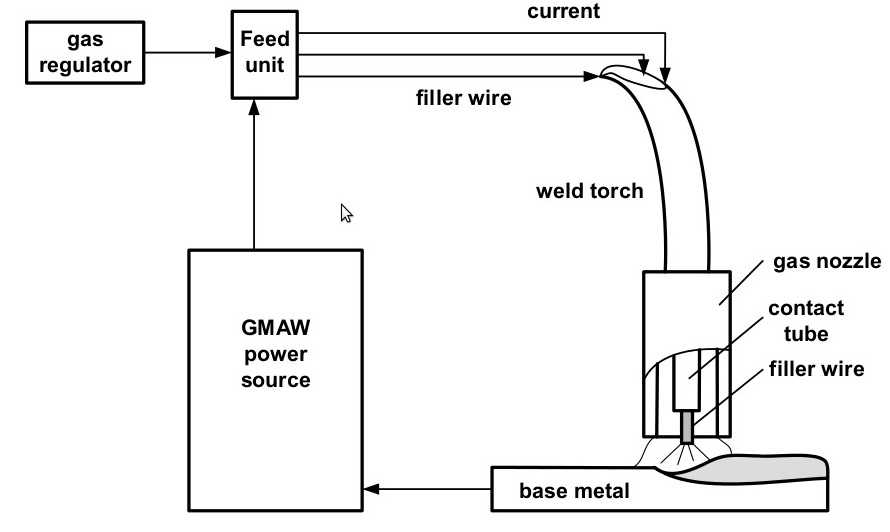
\includegraphics[width=9cm]{images/GMAW.png}
   \caption[Gas Metal Arc Welding]
   {Gas Metal Arc Welding \footnotemark[\value{footnote}]}  
\label{fig:img3}
\end{figure}

\begin{table}[]
\centering
\caption{Comparison of GMAW and GTAW welding}
\label{my-label}
\begin{tabular}{|c|c|c|}
\hline
                       & \textbf{GMAW}                                                                                                                                                  & \textbf{GTAW}                                                                                         \\ \hline
Power Sources          & Constant voltage type                                                                                                                                          & Constant current type                                                                                 \\ \hline
Electrodes             & Consumable type                                                                                                                                                & Non-consumable type                                                                                   \\ \hline
Current                & \begin{tabular}[c]{@{}c@{}}Direct current electrode positive\\  applied to weld head\end{tabular}                                                              & \begin{tabular}[c]{@{}c@{}}Direct current electrode negative\\ applied to weld head\end{tabular}      \\ \hline
Welding Speed          & \begin{tabular}[c]{@{}c@{}}A small increase in speed leads to \\ greater weld material penetration \\ but beyond a threshold leads to \\ undercut\end{tabular} & \begin{tabular}[c]{@{}c@{}}Changing welding speed \\ has no effect on quality of \\ weld\end{tabular} \\ \hline
Arc Length             & between 5-15mm                                                                                                                                                 & usually 2-5mm                                                                                         \\ \hline
Electrode Vertex angle & \begin{tabular}[c]{@{}c@{}}Usually kept at 45$\deg$ to normal\\  of the weld edge\end{tabular}                                                                & \begin{tabular}[c]{@{}c@{}}Angles between 30$\deg$ -\\ 120$\deg$\end{tabular}                       \\ \hline
\end{tabular}
\end{table}

\newpage
\subsection{Multi Robot Approaches for Welding}

One of the major drawbacks of robotic welding is the inability of the welding robot to manipulate the object. While for simple tasks, this does not pose a challenge, however for welding complex work pieces or for avoiding collision in the welding path, it becomes necessary to manipulate the object as well. In this section we will illustrate some of the well known and used approaches for multi robot welding. 
A well used approach to address this problem, is using two robots instead of one. A 6 dof manipulator is coupled with either a 2 dof rotary table or another 6 dof manipulator. It goes without saying that generating plans for more than one robot is a tedious task all the while maintaining the kinematic and dynamic constraints, as well as following the process parameters. In the next two subsections we will discuss about two popular multi robot planning and control approaches.

\subsubsection{Centralized and De-centralized planning}
A key point in designing multi robot planning approach is to generate motion plans centrally from either one robot or to use distributed planning with each robot planning its own path and then combining them to form a final plan. \\
In \cite{8}(Comparison of alternate methods for distributed motion planning of robot) the authors discuss a distributed planning approach based on artificial potential framework. The authors consider a case of planning path for three robots. The kinematic and dynamic model is formulated followed by the constraint relationship formulation as illustrated by \eqref{eq7},\eqref{eq8},\eqref{eq9}
\begin{equation}
\label{eq7}
\dot{q} = v
\end{equation}
\begin{equation}
\label{eq8}
M(q)\ddot{q} + V(q,\dot{q}) + G(q) = E(q)u - A^{T}\lambda
\end{equation}
\begin{equation}
\label{eq9}
M(q) = \begin{bmatrix} [M_{A}]_{2,2} & 0 & 0\\ 0 & [M_{A}]_{2,2}& 0\\ 0 & 0 & [M_{A}]_{2,2} \end{bmatrix},q = \begin{bmatrix} q_{A}\\ q_{B}\\ q_{C} \end{bmatrix}
\end{equation}
where $q=[x_{i} y_{i}]^{T} \epsilon \Re^{2}$
while the constraint equation is given as follows \eqref{eq10}
\begin{equation}
\label{eq10}
C(q) = \begin{bmatrix} (x_{A} - x_{B})^{2} + (y_{A} - y_{B})^{2} - {c_{AB}}^2\\ (x_{B} - x_{C})^{2} + (y_{B} - y_{C})^{2} - {c_{BC}}^2\\ (x_{C} - x_{A})^{2} + (y_{C} - y_{A})^{2} - {c_{CA}}^2 \end{bmatrix} = \begin{bmatrix} 0\\ 0\\ 0 \end{bmatrix}
\end{equation}
The authors then tested this model with independent parameterization and concluded that the projection based approach is robust but computationally expensive and which increases with each additional step. 

 
\subsubsection{Master Slave Configuration}
One of the major approaches for multi robot planning has been proposed in \cite{7}(kinematic cooperated welding trajectory planning) is master/slave cooperative planning. In this approach an initial kinematic relationship between the frames of the welding seam and the tool tip of the welding robots are established. One of the robots is considered as the master robot and its kinematic chain is defined from the base to its tool tip and for the slave robots the kinematic chain is defined from master robot base to slave robot base to slave robot tool and finally to master robot tool tip. The scheme is illustrated in illustration \ref{fig:img5}.
\begin{figure}[htbp] %  figure placement: here, top, bottom, or page
 \centering
   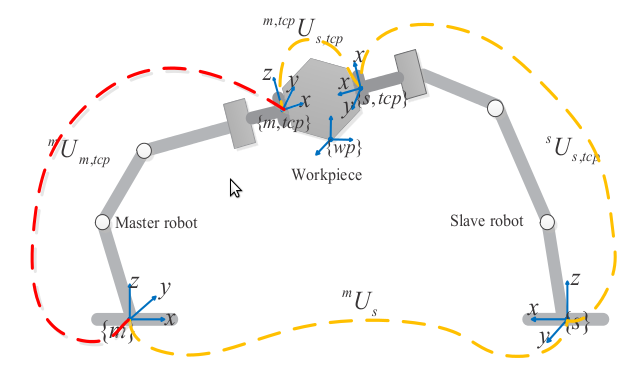
\includegraphics[width=9cm]{images/master_slave_coord.png}
   \caption[Master Slave Coordinate Specification]
   {Master Slave Coordinate Specification \footnotemark[\value{footnote}]}  
\label{fig:img5}
\end{figure}
Master slave configuration can be further divided into tightly coupled master/slave mode and loosely coupled master slave/mode. In tightly coupled master slave mode the master and slave robot assignments are fixed and in lightly coupled system the master slave assignments can be changed. 
The equation for a general master slave configuration is described in \eqref{eq12}, \eqref{eq13} describes a tightly couple master slave configuration and \eqref{eq14} describes the loosely coupled, time based master/slave configuration.
\begin{equation}
\label{eq12}
^{m}U_{m,tcp} = {^{m}U_{s}} \cdot ^{s}U_{s,tcp}\cdot^{s,tcp}U_{m,tcp}
\end{equation}
\begin{equation}
\label{eq13}
^{s}U_{s,tcp}(t) = {^{m}U_{s}}^{-1} \cdot ^{m}U_{m,tcp}(t)\cdot^{m,tcp}U_{s,tcp}
\end{equation}
\begin{equation}
\label{eq14}
^{s}U_{s,tcp}(t) = {^{m}U_{s}}^{-1} \cdot ^{m}U_{m,tcp}(t)\cdot^{m,tcp}U_{s,tcp}(t)
\end{equation}
The authors in \cite{7} then go onto describe three independent scenarios in which master/slave cooperative welding is applied. They are
\begin{enumerate}
\item Plate to plate welding - Welding tool tip of the multiple robots should have consistent relative distance.
\item Tube to plate welding - In this mode of operation, the robot which grips the work piece is considered master robot while the welding robot is configured in slave mode.
\item Tube-tube welding - This mode of operation is similar to tube to plate welding.
\end{enumerate}
Based on the results generated from running experiments for the three use cases, it was concluded that the methods described by the authors, achieve the desired goals successfully, however the actual performance of the methods are not reported. A key aspect of master/slave mode of operation that needs to be kept in mind is, for each welding task an accurate description of the seam to be welded needs to be formulated. For simple seam descriptions, this can be easily achieved, however for complex weld shapes the formulation becomes difficult. A counter approach to this is non-master slave approach which is described in \cite{6}.

In \cite{6}(Offline Kinematics Analysis and Path Planning of Two-Robot Coordination in Exhaust) the authors take two 6 dof robots and establish a coordinated planning based on non-master slave approach. 
The authors first establish a linked coordinate system for the two robots and the work piece as illustrated in figure \ref{fig:img4}.
\begin{figure}[htbp] %  figure placement: here, top, bottom, or page
 \centering
   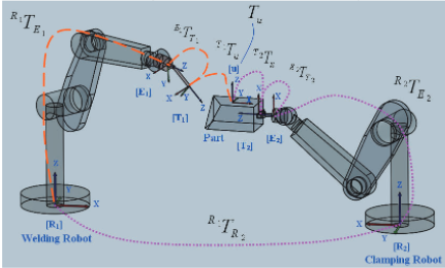
\includegraphics[width=9cm]{images/JointCoordinate2robs.png}
   \caption[Two Robot Coordinate System]
   {Two Robot Coordinate System \footnotemark[\value{footnote}]}  
\label{fig:img4}
\end{figure}
In non master/slave mode the pose of an object is set based on time. The mathematical description of the seams to be welded are specified based on which the transformations from robot 1 to work piece edge ${R1}^T_{E1} $ are calculated and similarly for robot 2 and work piece ${R2}^T_{E1}$. The seam to be welded is also described mathematically in this approach similar to \cite{7}. The kinematic scheme of the two robots and the work piece is illustrated with the following equation \eqref{eq15}.

\begin{equation}
\label{eq15}
{_{E_{1}}^{R_{1}}\textrm{T}} *{_{T_{1}}^{E_{1}}\textrm{T}} *{_{u}^{T_{1}}\textrm{T}} = {_{R_{2}}^{R_{1}}\textrm{T}} *{_{E_{2}}^{R_{2}}\textrm{T}}*{_{T_{2}}^{E_{2}}\textrm{T}} *{_{u}^{T_{2}}\textrm{T}} = _{u}T
\end{equation}

In \eqref{eq15} ${_{E_{i}}^{R_{i}}\textrm{T}} $ indicates the transformation matrix of end effector of robot i with respect to base of robot i. \\
the term ${_{T_{i}}^{E_{i}}\textrm{T}} $ indicates the transformation matrix of tool tip of robot i with respect to end effector i. \\ 
the term ${_{R_{2}}^{R_{1}}\textrm{T}} $ indicates the transformation matrix of robot 2 with respect to robot 1. \\ 
the term ${_{u}^{T_{i}}\textrm{T}} $ indicates the transformation matrix of work piece edge u with respect to tool tip i.\\
The authors conclude in the results section that using this approach will give the user greater capabilities to weld complex edges as the two 6 dof manipulators are more than enough to address collision avoidance and reachability issues. However a drawback of this method to be kept in mind is that for each edge to be welded, (no matter how complex it is geometrically) accurate mathematical description needs to be formulated. This greatly reduces flexibility for welding new edges. 

\newpage
\subsection{Welding as an Optimization Problem}
Current industrial are mostly pre-programmed and used to perform repetitive tasks. Hence they are unsuitable to be used in small and medium enterprises, where the welding tasks are flexible as the work piece itself may vary from task to task. It goes without saying that the welding process not only needs to be flexible but also needs to adapt based on the shape of the work piece to be welded. Furthermore it needs to finish the welding task in minimum time while consuming minimum resources (power, weld material) as well as ensuring optimal weld quality. This suggests that welding can be treated as an optimization problem with time to weld and motion cost as the cost functions; which are to be minimized. Two major approaches usually taken in this regard are 
\begin{enumerate}
\item Specify the optimization criteria as extra constraints and generate path plans subject to these additional constraints
\item Adding certain heuristics to existing planning algorithms to generate more optimized plans.
\end{enumerate}
The approaches are elaborated in the following sub sections.
\subsubsection{Welding Process Parameters Optimization}
In \cite{9}(weld quality assessment based on arc sensing), the authors propose a real time analysis of signals in frequency domain to give feedback to the robot controller in real time.The authors record current and voltage consumed during the welding process and then apply power spectral density and time frequency analysis methods to analyze them. The authors use Short Time Fourier Transform(SFTT) to analyze each frequency component of the recorded signals. The authors conducted extensive experiments and came to the conclusion that the developed system performs reasonably well, and is able to optimize the task and take into account any possible defects, however the performance is subject to constrains of accuracy of real time data collection and monitoring. Even though this method is computationally simple and easy to implement, but since the authors only test this method on geometrically simple welding tasks e.g. straight lines, it is difficult to truly gauge the performance of this optimization method. A similar method of regulating the current supplied to the weld tool tip to optimize the weld quality has been presented in \cite{10}(Effect of weld parameters on weld quality in sheet to tube..). The authors propose a method in which the current is varied with each point on the weld trajectory and the tensile strength of the weld spot is measured. From the experiments conducted the authors concluded that that as welding progresses the temperature of the weld surface increases and it results in reduced tensile strength of the weld surface. Also continuously increasing the current led to improvement in welding upto a certain level but beyond a certain point the effect of current became detrimental to the weld quality. Even though this paper lacks a model based approach, it provides key insight about the relationship of various parameters to weld quality.
In \cite{10}(Time optimal trajectory planning for a 6R..) the authors use a genetic algorithm based approach to optimize the trajectory generated for the robot. The authors first model the dynamics of the robot using standard kinematics and inverse kinematic equations. While applying the genetic algorithm, the following steps are taken
\begin{enumerate}
\item Fitness function: transforming the constraint equations into fitness functions
\item Determining the generic operators: since the authors use an adaptive genetic algorithm the crossover and mutation parameter change with each step so as to ensure the algorithm neither converges pre maturely nor it becomes too wide which leads to non convergence.
\item The initial, final and the middle points are determined through which the robot is expected to travel
\item Apply recursive trajectory planning for each segment
\item Apply adaptive genetic algorithm to compute the fitness function and produce the new generation.
\item Repeat until desired solution with value lesser than desired maximum cost is obtained
\item The final optimal trajectory for each section of the path is obtained along with the time required to traverse it.
\end{enumerate} 
The paper lack concrete experimentation and proper results of the experimentation has not been provide which makes it difficult to assess the actual performance of the adaptive genetic algorithm based approach. 
In \cite{12}(Simulation Planning of Robot Welding) the authors propose a method of process optimization in the following areas of a welding operation; robot location, weld gun selection and motion controlling.            
For weld gun selection the authors measure the suitability of the weld gun based on the size and shape of the work piece and the work space available as well as the reach-ability of the weld head in that particular work space. The selection can be made from x type and c type weld heads. Next the authors describe the positioning of the robot manipulator, tool tip, work piece object and other components of the weld cell, in the welding work space. The following diagram \ref{fig:img6} describes in brief the hierarchical structure followed in order to define the process.
\begin{figure}[htbp] %  figure placement: here, top, bottom, or page
 \centering
   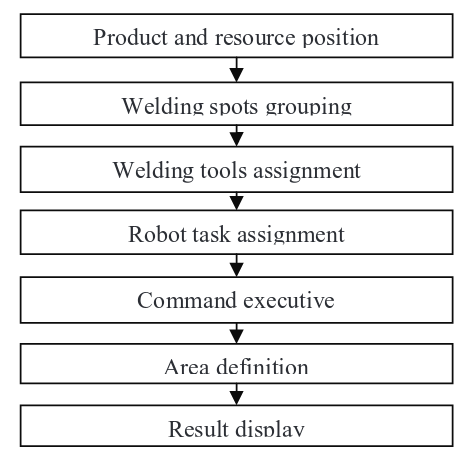
\includegraphics[width=9cm]{images/robotlocproc.png}
   \caption[Robot Location Model]
   {Robot Location Model \footnotemark[\value{footnote}]}  
\label{fig:img6}
\end{figure}
The product and resource position describe the positioning of the robots, work piece object, tool center point(TCP) and the weld gun. In welding spots grouping, the definition for the seam to be welded are defined. The tool to be assigned based on the work space is determined in welding tool assignment section. After the selection of the weld tool head and the work piece seam, the robot task is assigned. The task section contains definition of the work space in which the plan for the robot is to be generated usually in Cartesian coordinate system. It contains description of the weld seam and any collision objects, if present. After the plan is generated, it is executed on the robot inside the area definition. Finally the results of the planned path is displayed. \\ In the optimization section, the authors break down the final trajectory of the robot in basic motions -  such as joint, linear, circle and slew - which can be followed by the robot easily. After this step, the planned path is crash tested and modified accordingly. This paper lays the ground work for a hierarchical welding process model. However a lack of concrete implementation and subsequent testing leaves an open question about the feasibility of the described model. Few more papers on this topic have been evaluated in the later sections.

\subsubsection{Parameter Optimization of Motion Planning Algorithms}
In this section we will delve into work that focuses on optimizing the actual planner in order to generate optimal paths. In \cite{11}(HGRRT*) the authors propose an optimization based on user given input. The state cost definition is based on potential field framework. The planning algorithm minimizes motion cost by taking path segments with minimum cost while also optimizing the time required to generate the plan. In this approach the authors use a potential field function to guide the sampler of the RRT* algorithm to sample in used desired spaces. The state cost function is calculated using the following equation \eqref{11}
\begin{equation}
\label{16}
c(s) = \sum_{i} max(-\lambda_{i},0 ) + \lambda_{i}e^{\alpha_{i}d_{i}(s)^2} \epsilon (0,\sum_{i}|\lambda_{i}|]
\end{equation}
with $\lambda_{i} \epsilon \Re$ and $d_{i}(s)$ is the distance between work space and robot's reference point. The motion cost for the entire planned path is calculated based on the sequence of states with state costs with the following equation \eqref{16}
\begin{equation}
\label{17}
c(P) = \sum_{i=1}^{n-1}c(s_{i},s_{i+1})
\end{equation}
The proposed algorithm is illustrated as follows
\begin{itemize}
\item Sample: Random sample is generated in configuration space with probability 1 - $P_{goal}$ and for the goal state the probability is $P_{goal}$
\item Returns the k nearest neighbors of a state q. The value of k depends on dimension of configuration space.
\item Returns the path connecting initial state $q_{init}$ and goal state $q_{goal}$ composed by edges of the planning tree.
\item Collision free (q1, q2): Checks for collision between states q1 and q2 and returns the result.
\item Nearest: the closest node to q is returned. 
\item Cost: Returns the state cost of q
\item EdgeCost(q1, q2): Returns the cost between state q1 and q2
\end{itemize}
The authors conducted experiments and compared the results with TRRT algorithm. From the results it was concluded that the TRRT takes lesser time to find the solution path, however HGRRT* found shorter and more cost efficient paths. \\
Experimental optimization of welding parameters is an inefficient and ineffective method of doing so \cite{16}. The authors propose a Gaussian Process Regression Bayesian Optimization Algorithm(GPRBOA), in which the Gaussian Process Regression(GPR) is used to model non parametric complex welding process. Bayesian Optimization Algorithm(BOA) part is applied to balance the modeling and optimization processes. The welding parameters are described as a likelihood function as illustrated in \eqref{eq18}
\begin{equation}
\label{eq18}
\theta^{*} = argmax \log p(y|X,H,\theta)
\end{equation}
The final model, based on the welding parameters; generated after the GPR process is expressed in \eqref{19}
\begin{equation}
\label{eq19}
x^{*} = \arg max f(x), x* \epsilon X
\end{equation}
In this model, as soon as f(x) is generated, the problem is transformed into an optimization function, with the goal being to find the maximum value of $x^{*}$. Due to the reason the exploration and exploitation steps switch between each iteration, this algorithm is able to model the welding process online and optimize it online as well. Compared to other welding parameter optimization methods, this method was able to solve the correct parameter values in 7 iterations. A key point to be noted about this method is that being an online method, it has considerable risks of damaging either the robot or the work piece by drawing in more current, than the recommended amount. It is also difficult to judge from only one experiment whether the algorithm will be able to find out the optimal parameters in few iterations.
\newpage
\subsection{Robotic Welding Architecture and Planning in Abstract Space}
One of the major hindrance of using welding robots in industries is in the high cost associated with generation of new programs for welding robots\cite{14}(automatic program generation for welding robots..). A human user not only needs to have considerable knowledge of programming to be able to do this, it also requires a considerable time to reprogram a robot. A probable solution is to generate the robot programs offline and simulate the outcome before running the program on the robot. This ensures two things: (i) rectify any anomaly in the generated program contradictory to the desired outcome and (ii) optimize the program to ensure better performance of the robot, be it completing the welding task in lesser time or generating a more robust weld surface. In this section we  will discuss the various methodologies and platforms that exists for programming and simulating welding robots offline. 
\subsubsection{Program generation for Welding Robots and Simulation of Generated Plans}
In \cite{14} the authors divide the welding robot offline planning problem in two parts
\begin{enumerate}
\item Generating optimized plans for the tool tip within welding constraints. The authors define this as Task space or T-space motion planning.
\item Generating plans between robot home position and start and goal positions of the welding task. This is termed as configuration space planning problem.
\end{enumerate}
The general scheme of operation of the offline program generation is illustrated in the following diagram.
\begin{figure}[htbp] %  figure placement: here, top, bottom, or page
 \centering
   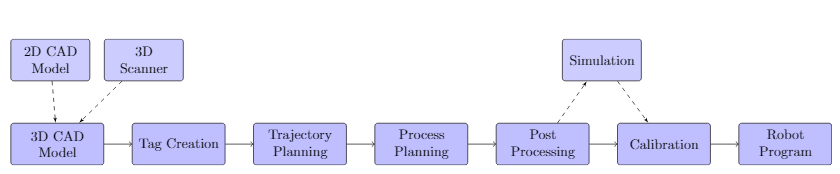
\includegraphics[width=9cm]{images/cadgen_model.png}
   \caption[Offline Weld Program Generation]
   {Offline Weld Program Generation \footnotemark[\value{footnote}]}  
\label{fig:img7}
\end{figure}
\newpage
The actual offline program is generated by the following steps
\begin{enumerate}
\item forward and inverse kinematic calculations
\item representing robots, work pieces and weld cell geometrically
\item manipulation and program generation
\item collision detection
\end{enumerate}
Tool Path Planning: The tool path planning space is defined with the following parameter
\begin{itemize}
\item t: the position along weld $t \epsilon [0,1]$
\item $\Re_{x,y,z} $ rotation around the X,Y,Z axes of tool tip
\item cfg: the robot kinematics is represented by $cfg \epsilon {1,2,...8}$
\item rail: position of the robot with respect to linear axis 
\end{itemize}
Motion Planning: The authors use Probabilistic Road Map(PRM) motion planner to generate plans to move the robot from home position and goal positions of the welds. Since the welds are simple paths the authors modified the sampling algorithm of the PRM planner to sample along a guided path without fully populating the tree so that the planner becomes faster. The sampling strategy is described in the following steps.
\begin{enumerate}
\item A Gaussian sampling strategy is used where two samples are generated close to the obstacle. If one sample is a collision free sample then it is added to the road-map. This results in sampling is performed close to the obstacles.
\item A number of points were generated close to the start and goal states to ensure they get connected to the roadmap.
\item Some additional points were generated in Cartesian space near weld spots to ensure that a solution is found.
\end{enumerate}
After the two planning stages the authors use a smoothing function to reduce jerky motions generated due to the PRM planner. This optimization resulted not only in smoother paths as well as reduced time for planning. From the results presented by the authors, it is seen that in some cases the planner fails however in most cases the planner is successful but the planning time for each plan varies greatly. \\
A similar model based approach is found in \cite{15}. The authors generate the CAD models of the work piece, robots and welding cell, which are then used in the simulation platform. The inverse and forward kinematic of each robot are calculated in a cyclical manner, and separately for each robot. The welding task is represented by a series of way points where each way point contains information about its own geometric position, the torch orientation and the robot's orientation. A search algorithm is then run through the way points to find a connecting path from the start to the goal point. The search algorithm works in the following four steps:
\begin{enumerate}
\item a line search is used to find an initial solution
\item if line search fails to find a solution an exhaustive search is launched
\item after a solutions is found the generated path is checked for discontinuities
\item a smoothing algorithm is applied to the generated path to reduce sharp movements of the manipulator
\end{enumerate}
The authors use RRT algorithm to plan path between weld points. The plan is directly generated in the Cartesian Space. A fast distance function from C-Space Toolkit computes the distance based on a distance function in order to generate collision free paths. The authors claimed that this approach has been used to successfully generate plans, however no experimentation results has been provided in the paper to back their claims or establish any performance evaluation. 
\subsubsection{Product, Process and Resource Model}
The solution architecture proposed in \cite{17} is presented as follows:
\begin{enumerate}
\item Product model - The product model, consists of the mathematical description of single or multiple-continuous joint seams of a welding work piece, which are selected by the user with a click. The user is able to select the desired edge to be welded from the CAD model.
\item Process model - The process model is a transformation from product
to process using Euler transformation. The description is performed in the workpiece
frame.
\item Resource model - The resource model contains kinematic and inverse kinematic
description of a 6 Dof industrial manipulator.
\end{enumerate}
After the selection of the welding task, the next step is calculation of motion cost, which is performed by the following algorithm \ref{algo1}:

\begin{algorithm}
		\caption{Optimal motion cost for collision avoidance for
robotic welding}
		\label{algo1}
        \textbf{Require:} $S_{1}=[k_{S1},\alpha_{S1}]$, $S_{2}=[k_{S2},\alpha_{S2}]$, 			$T_{W}^{proc_opt}(k)$ \\
        {Cost calculation for optimal welding angle}
		\begin{algorithmic}[1]
			\If{[$(Q2AA(T_{W}^{proc_opt}(k_{S1})) > \alpha_{S1}) \vee (Q2AA(T_{W}^{proc_opt}(k_{S2})) > \alpha_{S2})] \wedge [(Q2AA(T_{W}^{proc_opt}(k_{S1})) < \alpha_{S1}) \vee (Q2AA(T_{W}^{proc_opt}(k_{S2})) < \alpha_{S2})$]}
            	\State $RMP_{Opt} = \int_{k_{S1}}^{k_{S2}}Line(k).T_{W}^{proc_{opt}}(k)dk$
			\Else
            \State $[k_{c},\theta_{c}] \gets FindIntersection(Line(k),T_{W}^{proc_{opt}}(k))$
            \State $RMP_{Opt} = |\int_{k_{S1}}^{k_{c}}Line(k).T_{W}^{proc_{opt}}(k)dk| + |\int_{k_{c}}^{k_{S2}}Line(k).T_{W}^{proc_{opt}}(k)dk|$
            \EndIf \\
            {Cost calculation for for backward motion}
            \If{$(k_{S2}< k_{S1})$}
			\State $RMP_{Backward} = \infty$
            \Else
            \State $RMP_{Backward} = \emptyset$
            \EndIf
			\State $RMP_{Cost} = RMP_{Opt} + RMP_{Backward}$
		\end{algorithmic}
	\end{algorithm}
The current state of the art calculates the motion cost based on the angle of rotation from one weld state to another. A state validity checker is also implemented for collision checking and avoidance. Finally RRT* planner is used to solve the defined motion planning problem.
\subsubsection{Implementation Platform Architecture}
In this section we will briefly highlight the Product Process Resource model's implementation architecture.
\begin{figure}[htbp] %  figure placement: here, top, bottom, or page
 \centering
   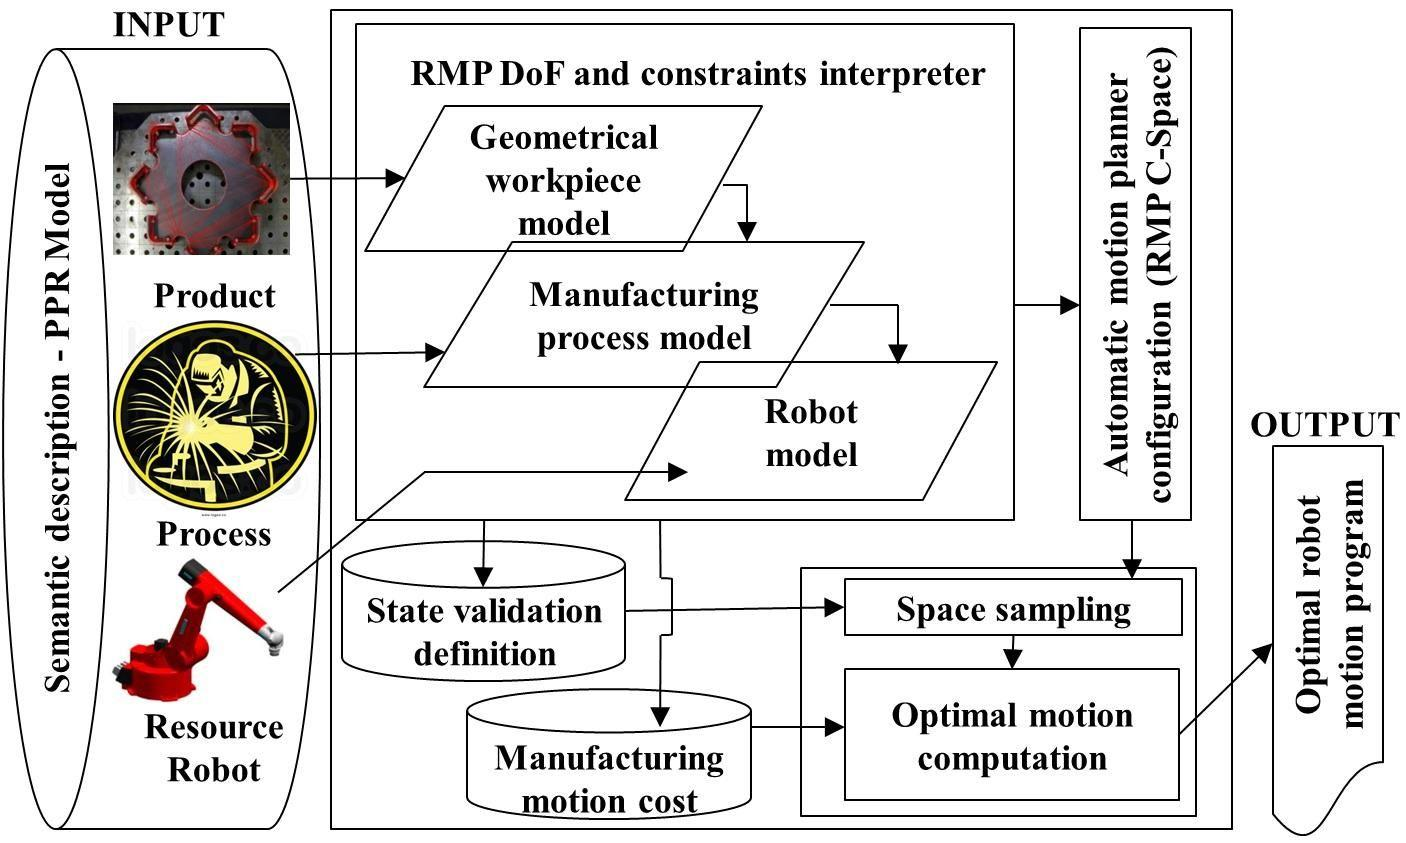
\includegraphics[width=9cm]{images/ppr_2.png}
   \caption[Product Process Resource(PPR) Architecture]
   { Product Process Resource(PPR) Architecture \footnotemark[\value{footnote}]}  
\label{fig:img8}
\end{figure}

The geometrical model of the work piece, the manufacturing process model and the robot model together create the automatic motion planning configuration space. A state validation model runs continuously to check for collisions, while the manufacturing motion cost model calculates the cost. Both of these data are fed to the motion planner, which then generates an optimized motion plan. 
\newpage
\newpage
\section{Problem formulation and Task description}
\label{sec:pf}
In this chapter, a list of problems or areas of improvements for (\citet{DiazP2016}) is identified and a model approach based on the literature survey of the previous section is presented. A detailed take on the problems and their respective implementations will be explained in the subsequent chapters.
\subsection{Problem formulation}
The following problems related to generating successful welding paths were identified:
\begin{itemize}
\item \textbf{Reachability:} A scenario is highlighting this is presented with the aid of the following diagram (\ref{fig:pf1}). In this scenario, we can see that the selected edge cannot be reached by the 6Dof manipulator. In order to generate a successful plan, which complies with the optimal definition, it is also necessary for the entire solution to lie in the dexterous work space of the 6 Dof manipulator.
\item \textbf{Deviation from optimal angle while avoiding collision:} In the following diagram(cite), we can observe that the weld tool tip follows an angle which is not in compliance with the optimal definition in order to avoid the collision. This leads to poor quality weld.
\item \textbf{Random Sampling:} The RRT* planner is a fast and efficient algorithm and guarantees  a solution asymptotically(cite and rephrase). However as we can see from the diagram below(cite), it generates a lot of random samples which do not at all contribute to finding a proper solution. Hence to make it more efficient, the problem of random sampling can be addressed.
\end{itemize}
\begin{figure}[!ht] %  figure placement: here, top, bottom, or page
	\centering
	\frame{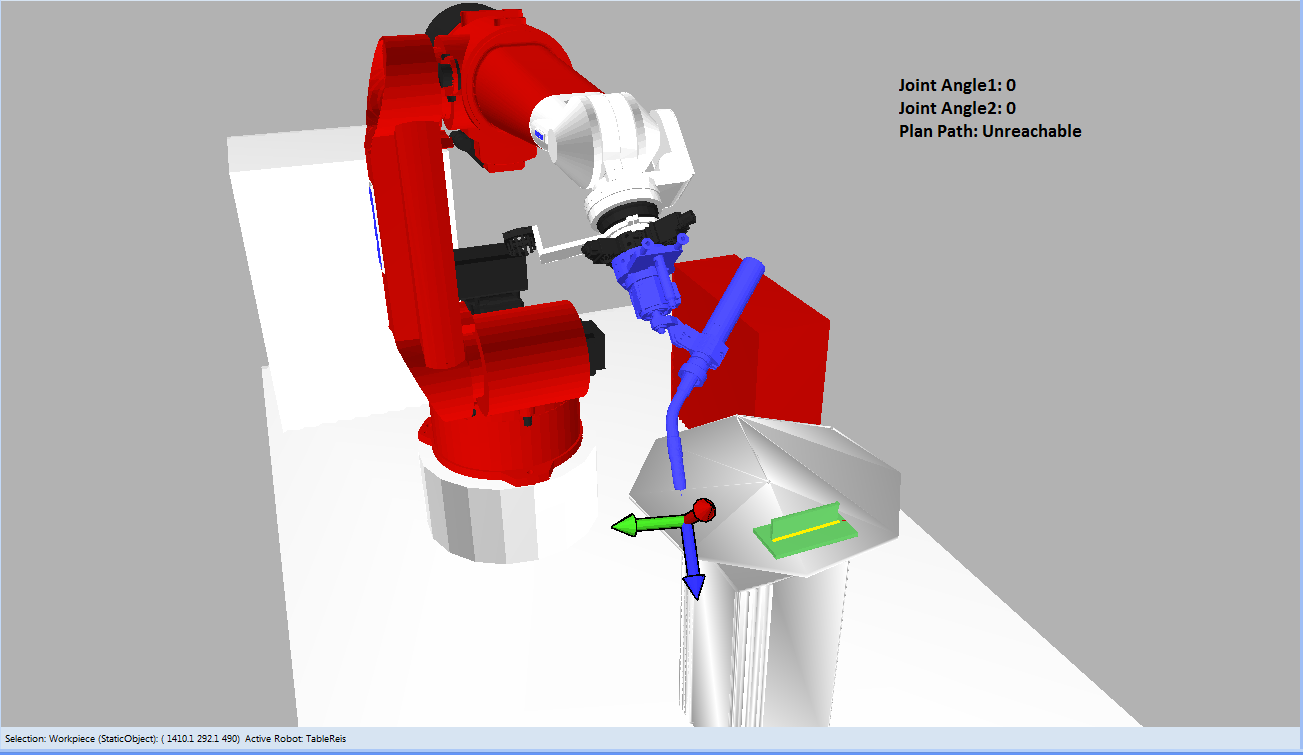
\includegraphics[width=0.8\textwidth,scale=0.6]{images/Urchbl_uscs.png}}
	\caption{Unreachable Use Case}
	\label{fig:pf1}
\end{figure} 

\subsection{Problem Approach Description}
In this section the proposed approach for the problems described above (\ref{sec:pf} is presented:

\begin{itemize}
\item \textbf{Incorporating a Rotary Table:} A rotary table can be considered as a 2 Dof which can provide extra degrees of freedom to tackle the problems of reachability and singularity. 
\item \textbf{Extending State Validity Checker:} In order to address the problems of reachability and singularity, we have to incorporate functions to detect reachability and link them to the state validity checker of the motion planner.
\item \textbf{Modeling of the Planning Space:} The introduction of the rotary table will create a more complex planning space. Generating a model for the same will help the user to visualize it as well as help to identify the gradient surface, which can be exploited to force the sampler to generate new samples in the areas with lower cost gradient thus ensuring an optimal solution.
\end{itemize}
\newpage
\section{Multi-Robot Approach for Weld Cost Minimization}
\localtableofcontents
In the problem formulation section(\ref{sec:pf}) we discussed how introduction of another robot can increase the number of degrees of freedom and hence allow the robot to perform more complex manipulations. Increasing the degree of complexity of motion can allow us to implement better optimization as well as solve the problems of unreachability and singularity. In this chapter we will discuss the integration of a 2 degrees of freedom rotary table into the existing architecture and how that is utilized to optimize the welding task. 

\subsection{Modeling the Rotary Table}
The existing implementation only contained kinematic description of the 6 axis manipulator with the weld tool tip. In the following subsections, we present a model of the 2 degree of freedom rotary table, along with the kinematic description and present the improved architectural model.
\subsubsection{Architecture of RobotKit}
The following architectural diagram(\ref{fig:img9}) has been color coded for better understanding. Blue represents the core functionalities of RobotKit. Red represents the kinematics and visualization models on which the improvements are implemented. Green represents external configuration files that are loaded inside RobotKit. Yellow represents the OMPL based planning library and pink represents the user interface block. \\
In the existing architecture the Kernel block creates instances of the kinematics and visualization models of the 6 Dof robot, which update the simulation environment based on the data input from the Information Exchange Pipeline. The planner interface class takes input from the kernel and the information exchange pipeline and user input for welding task. It then creates a planning problem and sends it to the OMPL based planning library. The communication between the planner interface and the planning library takes place using dll files. The project configuration file loads information about the dH parameters of the robot, position of the work piece and other relevant objects and in the weld cell. 

\begin{figure}[!htbp] %  figure placement: here, top, bottom, or page
 \centering
   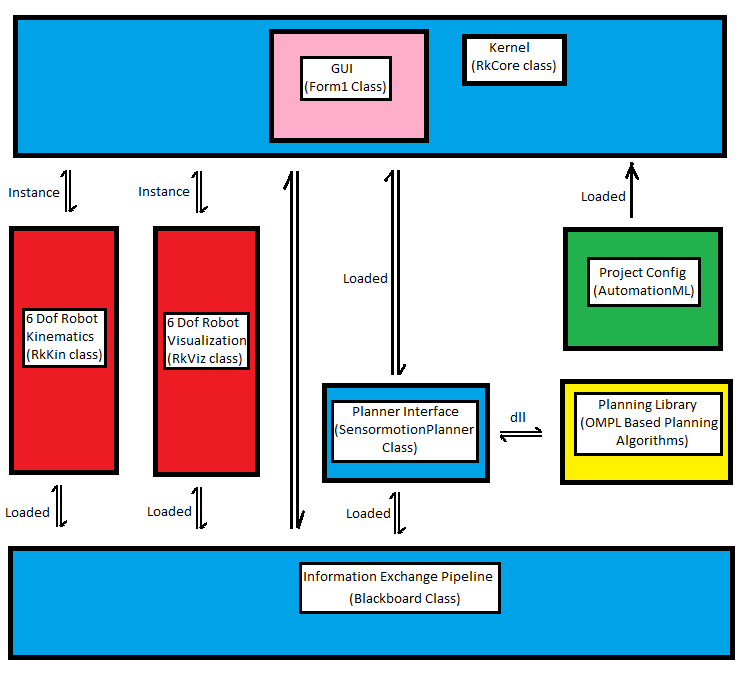
\includegraphics[width=9cm]{images/Original_arch.png}
   \caption[Exisitng Architecture of RobotKit[\citet{DiazP2016}]]
   {Exisitng Architecture of RobotKit[\citet{DiazP2016}]}  
\label{fig:img9}
\end{figure}

In the following architecture diagram (\ref{fig:img10}) the exact blocks which have been updated are highlighted. The kinematic and the visualization models now also includes definition of rotary table. The project configuration file (highlighted in green) has also been updated to include the dH parameters of the rotary table. 
\begin{figure}[!htbp] %  figure placement: here, top, bottom, or page
 \centering
   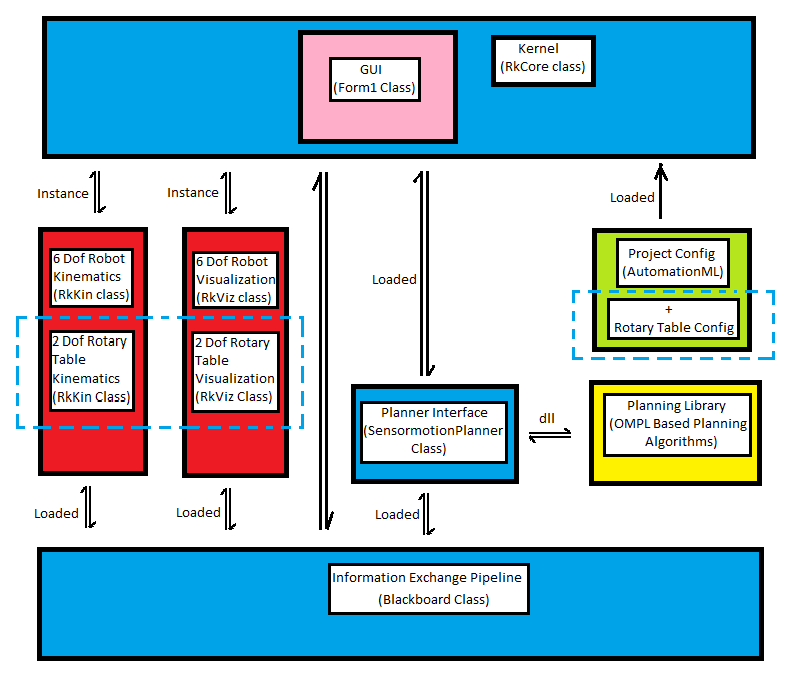
\includegraphics[width=9cm]{images/new_arch.png}
   \caption[Updated Architecture of RobotKit]
   {Updated Architecture of RobotKit[\citet{DiazP2016}]}  
\label{fig:img10}
\end{figure}
 

\subsubsection{Generating 3D Models for Simulation}
In order to update the simulation environment, 3D CAD models of the rotary table were created using  \hyperref{http://www.solidworks.com/}{Solidworks} software, based on the data-sheet specifications. In order to make the simulation mimic the real functioning of the rotary table, the table was divided into 3 separate CAD objects; base, middle joint and top plate. The images for the same are presented herewith. 

\begin{figure}[!htbp] %  figure placement: here, top, bottom, or page
\begin{subfigure}{\linewidth}
   \frame{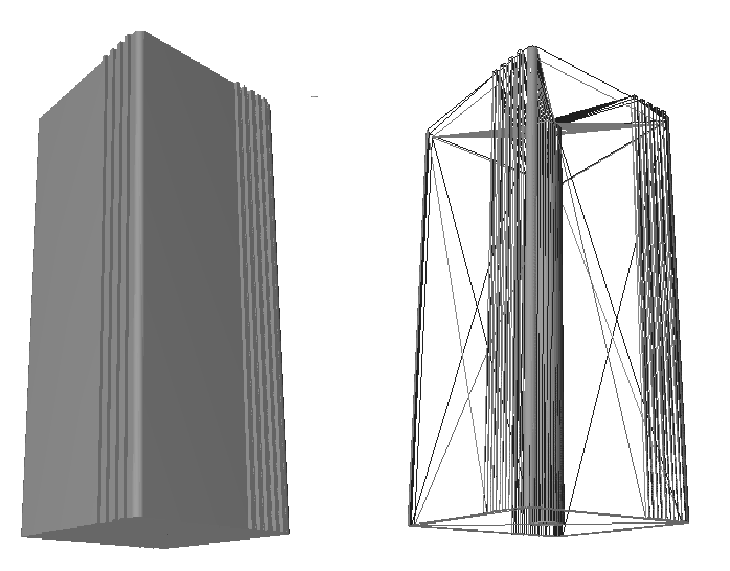
\includegraphics[width=.5\linewidth]{images/Base.png}}
   \frame{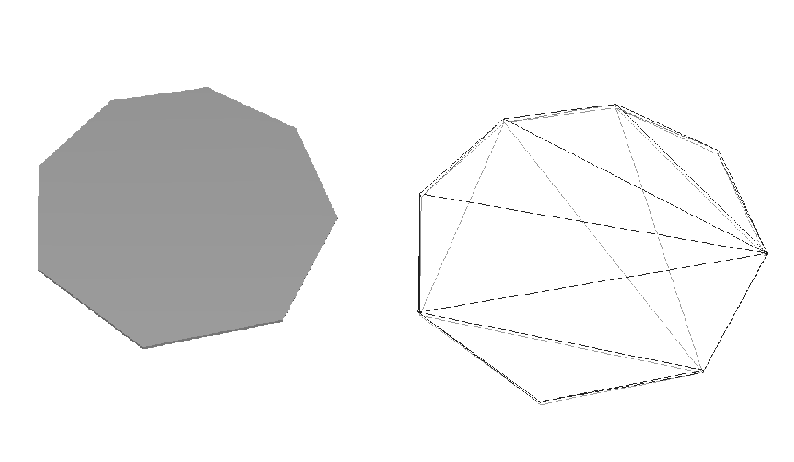
\includegraphics[width=.5\linewidth]{images/Top.png}}
      \caption[dd]{Base and Top Joint models}
   \end{subfigure}\par\medskip
   \begin{subfigure}{\linewidth}
   \centering
   \frame{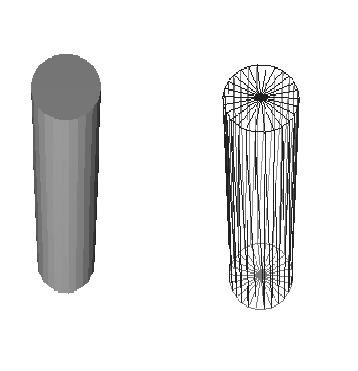
\includegraphics[width=.5\linewidth]{images/Mid.png}}
   \caption[dd]{Middle Joint model}
   \end{subfigure}
\caption[dd]{CAD models of the Rotary Table: Base, Middle and Top}
\label{fig:img11}
\end{figure}
 

\subsubsection{Kinematic Description of the Rotary Table}

The kinematic description of the 2 Dof Rotary table was created using the standard DH parameter approach. The DH parameters as specified in the Reis welding cell data-sheet are presented in the following table (\ref{tab2})
\begin{table}[!htbp]
\centering
\scalebox{1.2}{%
\frame{\begin{tabular}{@{}lllll@{}}
\toprule
i & $\alpha_{i-1}$ & a\_\{i-1\} & d\_\{i\} & $\theta_{i}$ \\ \midrule
1 & 0              & 0          & 0        & $\theta_{1}$ \\
2 & -90            & 0          & 150 mm     & $\theta_{2}$
\end{tabular}%
}}
\caption{DH parameter of Rotary Table}
\label{tab2}
\end{table}
\\
The next step is to construct the link frames of the joints of the table in accordance with the approach mentioned in [\citet{craig2005introduction}]. The frames were plotted in Cartesian space with actual values from the real robot system. The values are the actual coordinates of the joint with respect to the global coordinate frame. Since the rotary table present in the welding cell has 2 Dof, we take Joint 0 as a reference frame, which coincides with the frame of Joint 1. According to the Reis welding cell data-sheet(use cite doc), the axis of rotation of Joint 1 of the rotary table is same as the X axis of the robot frame of the 6 dof manipulator and the axis of rotation of Joint 2 is same as the Z axis of the robot frame of the 6 dof manipulator. \\
In the following figure \ref{fig:img12} the world and robot frames along with the joint frames of the rotary table in the Cartesian coordinate frame are plotted. 
\begin{figure}[!htbp] %  figure placement: here, top, bottom, or page
 \centering
   \frame{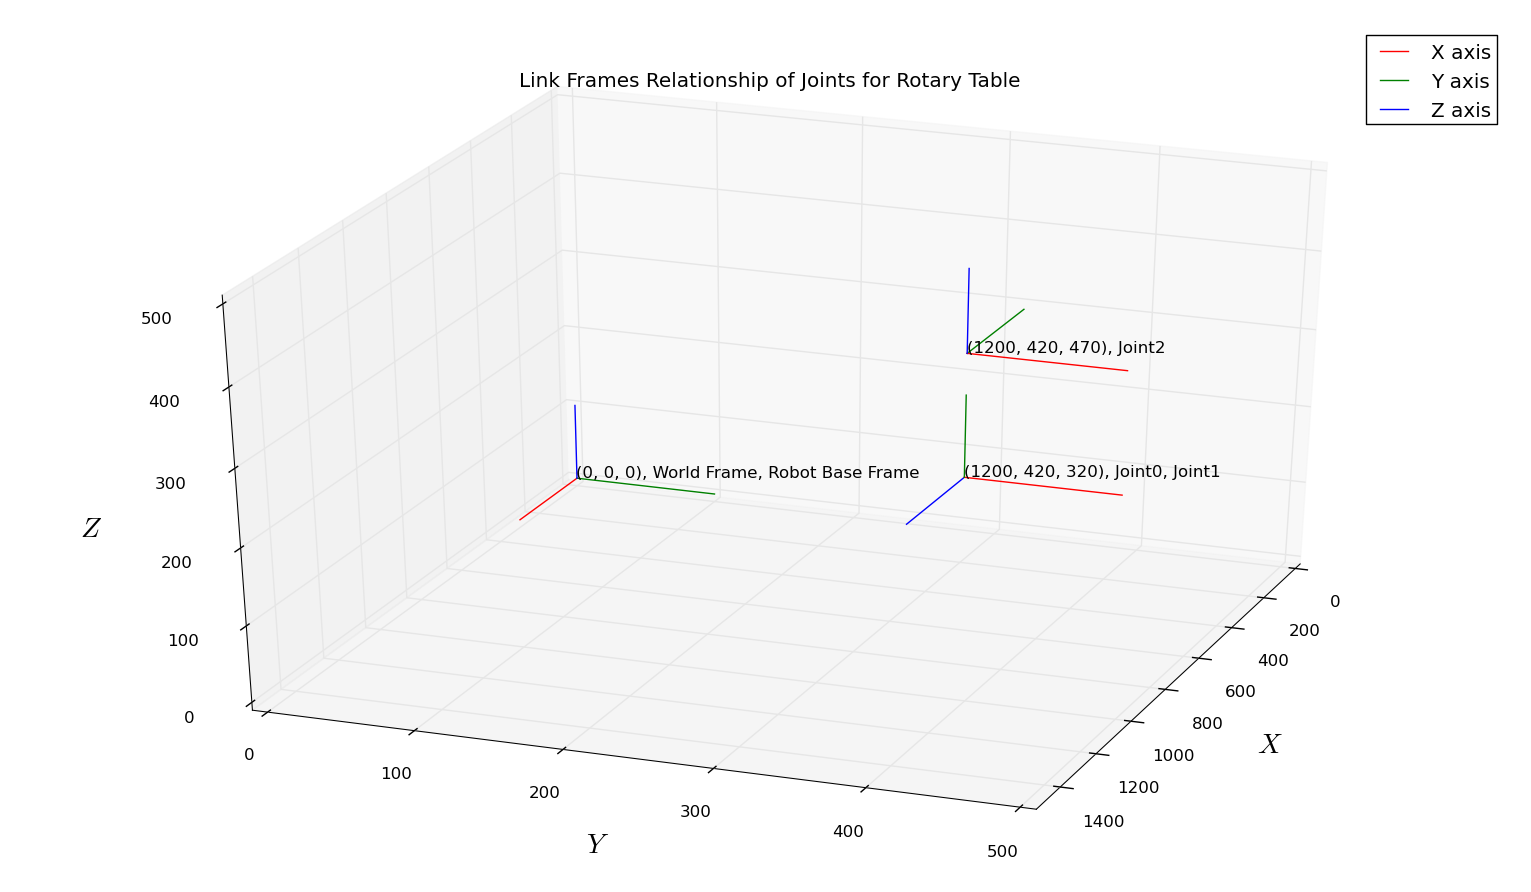
\includegraphics[width=12cm]{images/Frames_jnttab.png}}
   \caption{Link Frame Relationship of Joints of Rotary Table}  
\label{fig:img12}
\end{figure}

Based on the DH parameters from table \ref{tab2} we now construct the forward kinematic chain. 
\begin{equation}
\label{eq20}
_{0}^{1}\textrm{T} = \begin{bmatrix} \cos\theta_{i} & -\sin \theta_{i} & 0 & 0\\ \sin \theta_{i} & \cos \theta_{i} & 0 & 0\\ 0 & 0 & 1 & 0\\ 0 & 0 & 0 & 1 \end{bmatrix}
\end{equation}

\begin{equation}
\label{eq21}
_{2}^{1}\textrm{T} = \begin{bmatrix} \cos\theta_{i} & -\sin \theta_{i} & 0 & 0\\ 0 & 0 & 1 & 150\\ -\sin \theta_{i} & -\cos\theta_{i} & 0 & 0\\ 0 & 0 & 0 & 1 \end{bmatrix}
\end{equation}

\begin{equation}
\label{eq22}
\textrm{T}_{table} =_{2}^{0}\textrm{T}_{1}^{0}\textrm{T}._{2}^{1}\textrm{T} = \begin{bmatrix} \cos^{2}\theta_{i}& -\cos\theta_{i}.\sin\theta_{i} & -\sin\theta_{i} & -150*\sin\theta_{i}\\ \cos\theta_{i}.\sin\theta_{i} & -\sin^{2}\theta_{i} & \cos\theta_{i} & 150*\cos\theta_{i}\\ -\sin\theta_{i} & -\cos\theta_{i}& 0 & 0\\ 0& 0& 0& 1\end{bmatrix}
\end{equation}

\subsubsection{Workpiece Transformation}

Since the main objective of moving the rotary table is to move the work piece, a transformation function is also necessary to simulate the changed position of the work piece in accordance with the motion of the table. It is to be noted that we can only read the position and orientation information of the workpiece, so it was necessary to convert it into a transformation matrix and recalculate the position and orientation values from the matrix when returning the values to the software.
The terms of the algorithm are defined as follows:
\begin{itemize}
	\item $_{T}^{W}T$ $\rightarrow$ Transformation of Table frame with respect to World frame
	\item $_{WP}^{W}P$ $\rightarrow$ Transformation of Workpiece frame with respect to World frame
	\item $_{T}^{W}T_{new}$ $\rightarrow$ Transformation of rotated Table frame with respect to World frame
	\item $_{WP}^{T}T_{ref}$ $\rightarrow$ Transformation of initial/reference Workpiece frame with respect to Table frame
	\item $_{WP}^{W}T_{new}$ $\rightarrow$ Transformation of workpiece from new position with respect to world frame.
\end{itemize} 

\begin{algorithm}[!htbp]
	\caption{Transformation of Work Piece position wrt Table Position}
	\label{algo2}
	\textbf{Given:} $ \text{Original }(\textit{$_{T}^{W}P$}, \textit{$_{T}^{W}O$})\text{pose and orientation information}  \bigwedge \text{ new}\\(\textit{$_{T}^{W}P_{new}$}, \textit{$_{T}^{W}O_{new}$}) \text{pose and orientation information} \text{ of table wrt. to world frame }\\ \text{ and current position and orientation } (\textit{$_{WP}^{W}P$}, \textit{$_{WP}^{W}O$}) \text{information of work piece wrt.} \\ \text{world frame} $ \\ \\
	\textbf{Output:} $\text{New}(\textit{$_{WP}^{W}P_{new}$},\textit{$_{WP}^{W}O_{new}$}) \text{position and orientation  information} \\ \text{of work piece wrt. world frame}$\\
	
	\begin{algorithmic}[1]
		\State $\textit{$_{T}^{W}T$} \gets Converttomatrix(\textit{$_{T}^{W}P$},\textit{$_{T}^{W}O$})$
		\State $\textit{$_{WP}^{W}P$} \gets Converttomatrix(\textit{$_{WP}^{W}P$},\textit{$_{WP}^{W}O$})$
		\State $\textit{$_{T}^{W}T_{new}$} \gets Converttomatrix(\textit{$_{T}^{W}P_{new}$}, \textit{$_{T}^{W}O_{new}$})$ \\
		\If{[${Initializing program}$]}
		\State $\textit{$_{WP}^{T}T_{ref}$} \gets \textit{$_{T}^{W}T^{-1}$} * \textit{$_{WP}^{W}T$}$
		\EndIf \\
		\If{[$\text{user offset work piece position}$]}
		\State $\textit{$_{WP}^{T}T^{'}$} \gets \textit{$_{T}^{W}T^{-1}$} * \textit{$_{WP}^{W}T^{'}$}$
		\State $\textit{$_{WP}^{T}T_{ref}$} \gets $\textit{$_{WP}^{T}T^{'}$}
		\EndIf \\
		
		\State $\textit{$_{WP}^{W}T_{new}$} \gets \textit{$_{T}^{W}T_{new}^{-1}$} * \textit{$_{WP}^{T}T_{ref}$}$\\
		\State $\textit{$_{WP}^{W}P_{new}$} \gets position(\textit{$_{WP}^{W}T_{new}$})$
		\State $\textit{$_{WP}^{W}O_{new}$} \gets matrixtoeulerangles(\textit{$_{WP}^{W}T_{new}$})$\\
		\If{[$Edge to be welded selected$]}
		\State $SelectedEdgeTransform()$
		\EndIf \\
		\textbf{return:} $\textit{$_{WP}^{W}P_{new}$},\textit{$_{WP}^{W}O_{new}$}$
	\end{algorithmic}
\end{algorithm}
\newpage
\subsubsection{Selected Edge Transformation}
The selected edge is defined with start and goal points. It is to be noted that we can only read the position and orientation information of the selected edge points, so it was necessary to convert it into a transformation matrix and recalculate the position and orientation values from the matrix when returning the values to the software.
\begin{itemize}
	\item $_{T}^{W}T$ $\rightarrow$ Transformation of Table frame with respect to World frame
	\item $_{WP}^{W}P$ $\rightarrow$ Transformation of Workpiece frame with respect to World frame
	\item $_{T}^{W}T_{new}$ $\rightarrow$ Transformation of rotated Table frame with respect to World frame
	\item $_{SP}^{WP}T$ $\rightarrow$ Transformation of start point of selected edge with respect to workpiece frame 
	\item $_{GP}^{WP}T$ $\rightarrow$ Transformation of goal point of selected edge with respect to workpiece frame
	\item $_{SP}^{WP}T_{ref}$ $\rightarrow$ Transformation of initial/reference start point frame with respect to workpiece frame
	\item $_{GP}^{WP}T_{ref}$ $\rightarrow$ Transformation of initial/reference goal point frame with respect to workpiece frame
\end{itemize} 
\begin{algorithm}
	\caption{Transformation of Selected Edge with respect to Work Piece Position}
	\label{algo3}
	\textbf{Given:} $ \text{Original pose and orientation information of start(\textit{$_{SP}^{W}P$}, \textit{$_{SP}^{W}O$}) and goal} \\ \text{points(\textit{$_{GP}^{W}P$}, \textit{$_{GP}^{W}O$}) }  \bigwedge \text{ new}(\textit{$_{WP}^{W}P_{new}$}, \textit{$_{WP}^{W}O_{new}$}) \text{pose and orientation information} \\ \text{ of work piece wrt. to world frame } \text{ and old position and orientation }\\ (\textit{$_{WP}^{W}P$}, \textit{$_{WP}^{W}O$}) \text{information of work piece wrt. world frame} $ \\ 
	\textbf{Output:} $\text{New pose and orientation information of start(\textit{$_{SP}^{W}P_{new}$}, \textit{$_{SP}^{W}O_{new}$}) and } \\ \text{goal points(\textit{$_{GP}^{W}P_{new}$}, \textit{$_{GP}^{W}O_{new}$}) }$\\
	
	\begin{algorithmic}[1]
		\State $\textit{$_{SP}^{W}T$} \gets Converttomatrix(\textit{$_{SP}^{W}P$},\textit{$_{SP}^{W}O$})$
		\State $\textit{$_{GP}^{W}T$} \gets Converttomatrix(\textit{$_{GP}^{W}P$},\textit{$_{GP}^{W}O$})$
		\State $\textit{$_{WP}^{W}T$} \gets Converttomatrix(\textit{$_{WP}^{W}P$},\textit{$_{WP}^{W}O$})$
		\State $\textit{$_{WP}^{W}T_{new}$} \gets Converttomatrix(\textit{$_{WP}^{W}P_{new}$}, \textit{$_{WP}^{W}O_{new}$})$ 
		\For{[$each selected edge$]} 
		\If{[${Initializing program}$]}
		\State $\textit{$_{SP}^{WP}T_{ref}$} \gets \textit{$_{WP}^{W}T^{-1}$} * \textit{$_{SP}^{W}T$}$
		\State $\textit{$_{GP}^{WP}T_{ref}$} \gets \textit{$_{WP}^{W}T^{-1}$} * \textit{$_{GP}^{W}T$}$
		\EndIf 
		\If{[$\text{user offset work piece position}$]}
		\State $\textit{$_{SP}^{WP}T^{'}$} \gets \textit{$_{WP}^{W}T_{new}^{-1}$} * \textit{$_{SP}^{W}T$}$
		\State $\textit{$_{GP}^{WP}T^{'}$} \gets \textit{$_{WP}^{W}T_{new}^{-1}$} * \textit{$_{GP}^{W}T$}$
		\State $\textit{$_{SP}^{WP}T_{ref}$} \gets $\textit{$_{SP}^{WP}T^{'}$}
		\State $\textit{$_{GP}^{WP}T_{ref}$} \gets $\textit{$_{SP}^{WP}T^{'}$}
		\EndIf 		
		\State $\textit{$_{SP}^{W}T_{new}$} \gets \textit{$_{WP}^{W}T_{new}^{-1}$} * \textit{$_{SP}^{WP}T_{ref}$}$
		\State $\textit{$_{GP}^{W}T_{new}$} \gets \textit{$_{WP}^{W}T_{new}^{-1}$} * \textit{$_{GP}^{WP}T_{ref}$}$
		
		\State $\textit{$_{SP}^{W}P_{new}$} \gets position(\textit{$_{SP}^{W}T_{new}$})$
		\State $\textit{$_{SP}^{W}O_{new}$} \gets matrixtoeulerangles(\textit{$_{SP}^{W}T_{new}$})$
		\State $\textit{$_{GP}^{W}P_{new}$} \gets position(\textit{$_{GP}^{W}T_{new}$})$
		\State $\textit{$_{GP}^{W}O_{new}$} \gets matrixtoeulerangles(\textit{$_{GP}^{W}T_{new}$})$\\
		
		\EndFor \\
		\textbf{return:} $\textit{$_{SP}^{W}P_{new}$},\textit{$_{SP}^{W}O_{new}$},\textit{$_{GP}^{W}P_{new}$},\textit{$_{GP}^{W}O_{new}$}$
	\end{algorithmic}
\end{algorithm}
\newpage
\subsection{Cost Function Formulation}
\label{ssec:cst}
Two different cost functions (sections\ref{sssec:tcpcst} and \ref{sssec:jntcst}) were formulated and finally a weighted combination of the two (section \ref{sssec:aggcst})was created, to form the final cost function. The plots of the cost functions were created by running the planner for every different orientations of the table for the following two work pieces. For each workpiece 2 edges were randomly selected to demonstrate the behaviors based on the cost function definition. The edges also contain the convention definition, which specifies the alignment of the TCP with respect to the selected edge. For example in \ref{fig:imgoridef1} and \ref{fig:imgoridef2}, the TCP moves along the planned path in accordance with the convention; the X axis (marked by red) points from start to goal point along the edge to be welded, and the Y (marked by green) and Z (marked by blue) maintain an angle of 45$^{\circ}$ with respect to the selected edge. \\
\begin{figure}[!htbp] %  figure placement: here, top, bottom, or page
	\centering
	\begin{subfigure}[b]{0.4\textwidth}
		\frame{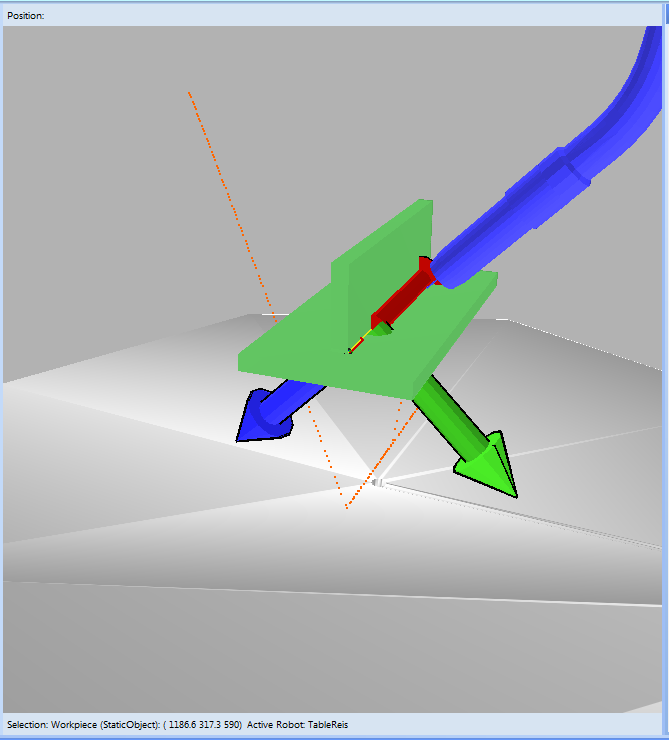
\includegraphics[width=1\textwidth,height=0.2\textheight]{images/tcp_ori.png}}
		\caption{}
		\label{fig:imgoridef1}
	\end{subfigure}
	\begin{subfigure}[b]{0.4\textwidth}
		\frame{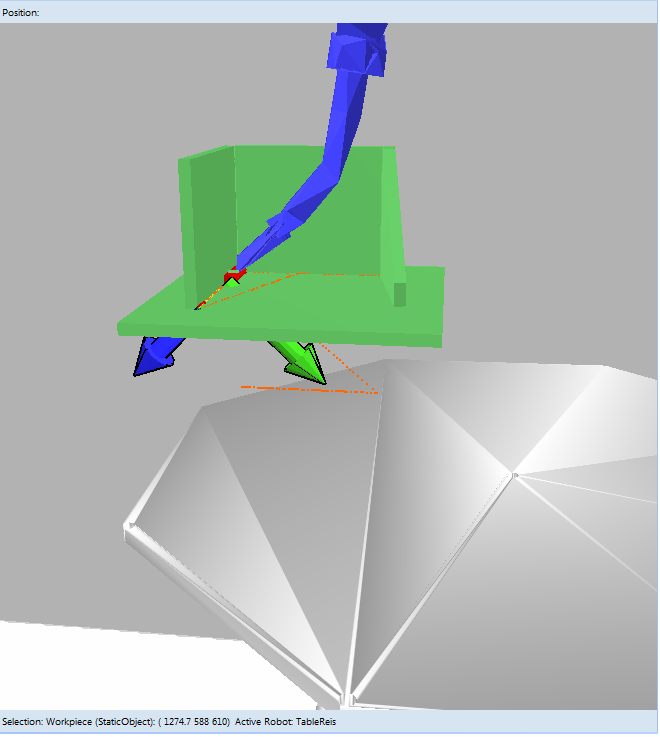
\includegraphics[width=1\textwidth,height=0.2\textheight]{images/tcp_ori_al.png}}
		\caption{} 
		\label{fig:imgoridef2}
	\end{subfigure}	
	\caption{Convention Definition of TCP with Respect  to Weld Edge}  
	\label{fig:tcor}
\end{figure}

\begin{figure}[!htbp] %  figure placement: here, top, bottom, or page	
	\centering
	\begin{subfigure}[b]{0.4\textwidth}	
		 \frame{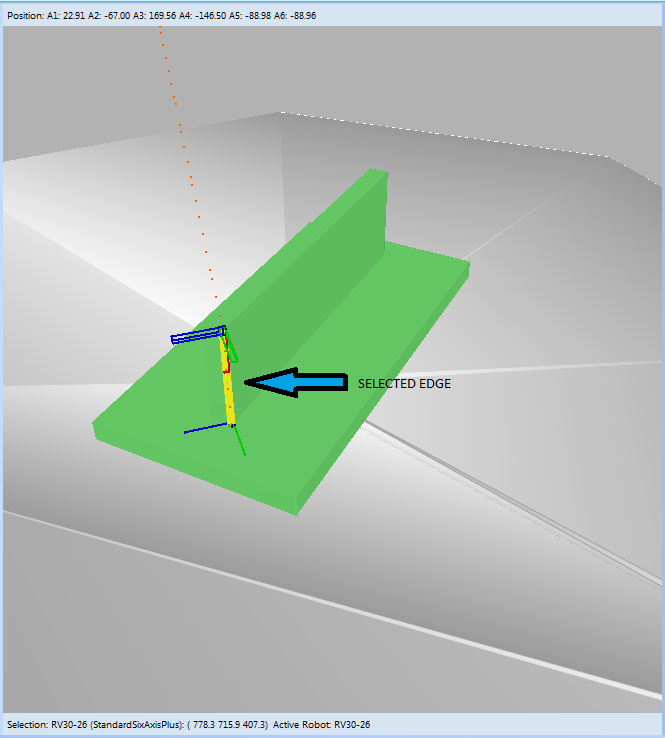
\includegraphics[width=1\textwidth,height=0.2\textheight]{images/normwp_left.png}}
		 \caption{Left Vertical Edge of T-Joint Workpiece}
		\label{fig:imguc1}
	\end{subfigure}
	\begin{subfigure}[b]{0.4\textwidth}		
		\frame{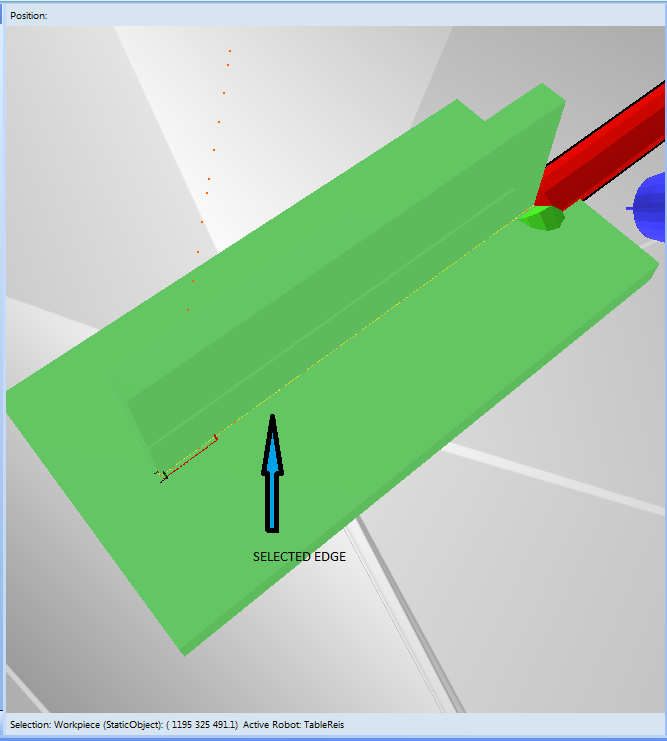
\includegraphics[width=1\textwidth,height=0.2\textheight]{images/normwp_flat.png}}
		\caption{Horizontal Edge of T-Joint Work  piece} 
	\label{fig:imguc2}
	\end{subfigure}		
	\caption{Simple T-Joint Workpiece}  
	\label{fig:uc1}
\end{figure}
\textbf{1st Use Case:}This \ref{fig:uc1} is a T-Jointed work piece for which we select two edges, to demonstrate the two different cost functions. The edges for which weld paths are to be generated are marked by yellow lines and pointed at by the arrows

\textbf{2nd Use Case:}The welding robot was demonstrated in Automatic Messe 2016(Munich) in which this(\ref{fig:uc2}) work piece was used to demonstrate the autonomous program generation for welding. For this workpiece, two edges were considered, which are marked yellow lines and pointed at by the arrows.
\begin{figure}[!htbp] %  figure placement: here, top, bottom, or page
	\centering
	\begin{subfigure}[b]{0.4\textwidth}
		\frame{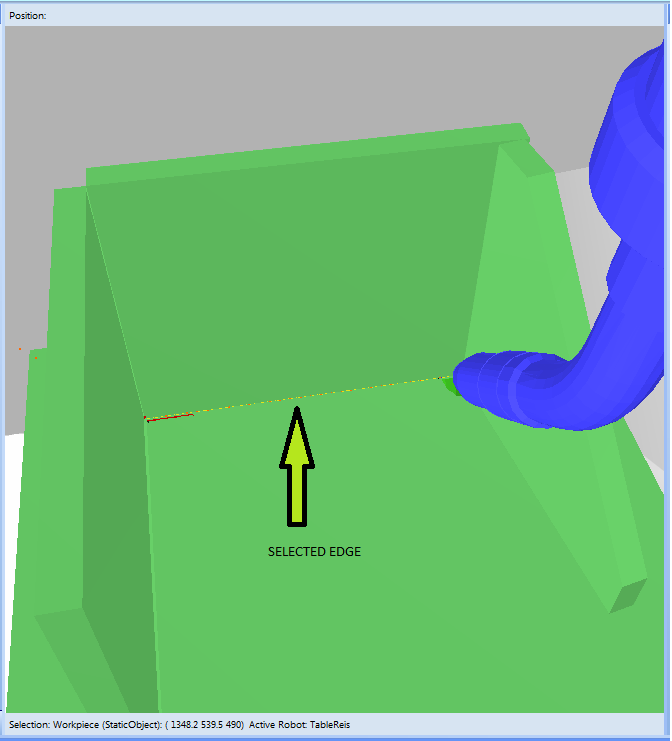
\includegraphics[width=1\textwidth,height=0.2\textheight]{images/auto_flat.png}}
		\caption{Horizontal Edge of Automatica 2016 Workpiece}  
		\label{fig:imguc3}
	\end{subfigure}
	\begin{subfigure}[b]{0.4\textwidth}
		\frame{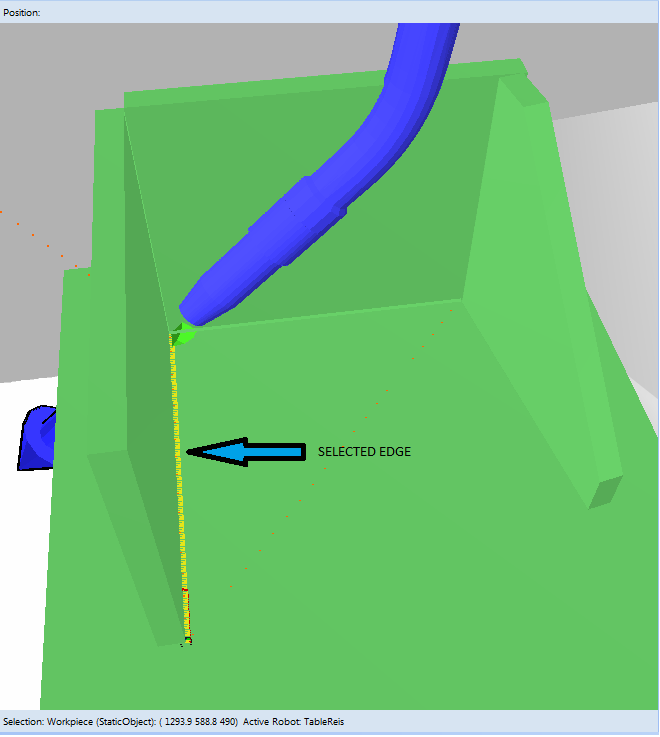
\includegraphics[width=1\textwidth,height=0.2\textheight]{images/auto_left.png}}
		\caption{Inner Left Edge of Automatica 2016 Workpiece}  
		\label{fig:imguc4}
	\end{subfigure}	
\caption{Workpiece used in Automatica 2016 demonstration}
\label{fig:uc2}
\end{figure}

\subsubsection{Difference of TCP orientation and Workpiece edge}
\label{sssec:tcpcst}
In (\ref{fig:tcor}) we saw the relationship between TCP orientation and the workpiece convention. In order to generate high quality weld paths, it is necessary to orient the TCP in accordance with the optimal TCP orientation definition. Therefore for our first cost function definition; we consider the difference between the actual TCP orientation and the optimal welding process defined TCP orientation [\citet{DiazP2016}]. The greater the difference, higher the cost and vice-versa. The difference of the quaternions is calculated using the following steps as defined in [\citet{DiazP2016}].
\begin{itemize}
	%content...
	\label{algo4ppr}
	\item Both the sets of quaternions are defined using the standard convention og 4 quaternion components namely: $q1,q2,q3,q4$
	\item Calculate the normal of optimal and actual quaternion values.
	\item Calculate the inverse of the normalized optimal quaternion and multiply with the normalized actual quaternion to obtain the difference of the quaternions.
	\item Convert the difference of the quaternions into an angle value.
	\item Ensure difference angle lies within -180$^{\circ}$ and 180$^{\circ}$
	\item return $C_{tcp}$(\textit{Solution})
\end{itemize}
In order to analyze the cost function, it was necessary to plot the cost values generated for each welding path for various orientation of the table. We considered a range of -80$^{\circ}$ to +80$^{\circ}$ for 1st joint angle and -140$^{\circ}$ to 140$^{\circ}$ for 2nd joint angle of the table. Plots for both use cases; as illustrated in figures \ref{fig:uc1} and \ref{fig:uc2}
were generated.
\begin{figure}[!htbp] %  figure placement: here, top, bottom, or page
	\centering
	\begin{subfigure}[b]{0.4\textwidth}
		\frame{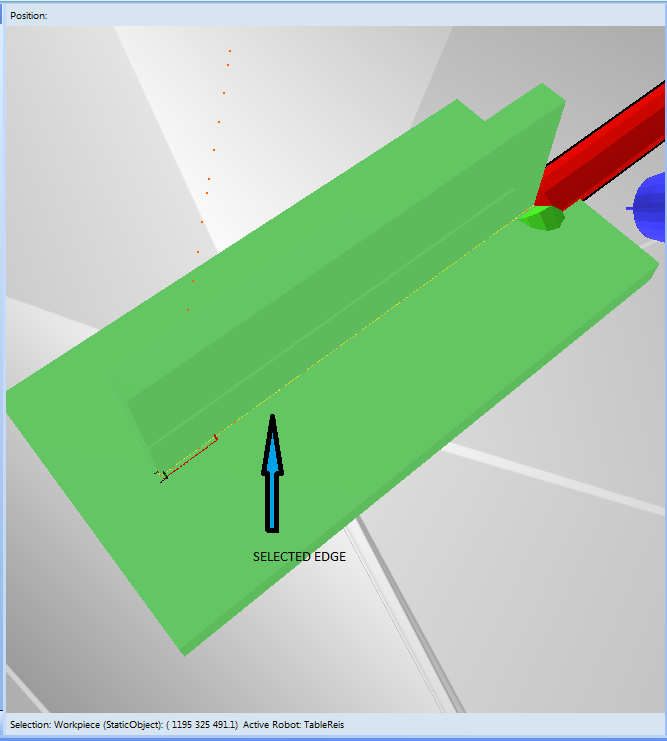
\includegraphics[width=1\textwidth,height=0.2\textheight]{images/normwp_flat.png}}
		\caption{Edge to be welded}  
		\label{fig:cp1b}
	\end{subfigure}
	\begin{subfigure}[b]{0.4\textwidth}
		\frame{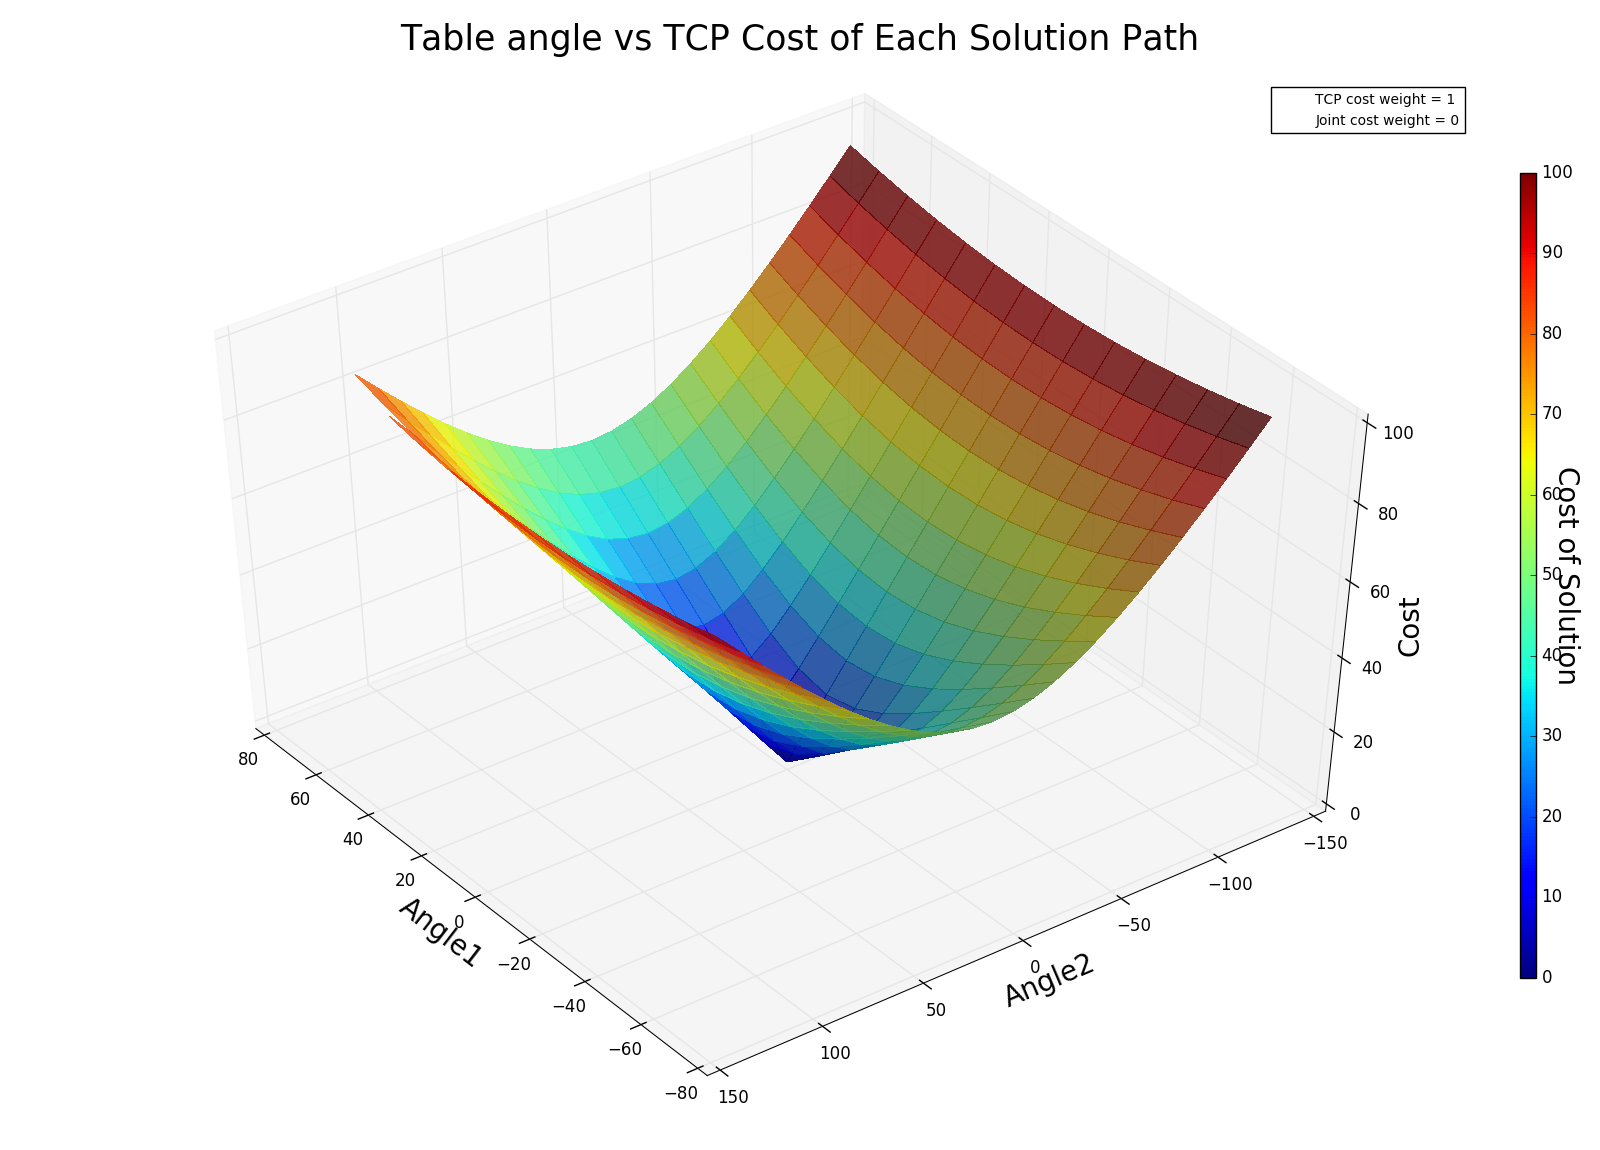
\includegraphics[width=1\textwidth,height=0.2\textheight]{images/orihori_tcpcst.png}}
		\caption{Cost Function Plot}  
	\label{fig:cp1a}
	\end{subfigure}	
	\caption{Cost Function Plot of T-Jointed workpiece: TCP orientation}
	\label{fig:cp1}
\end{figure}
\\
The edge to be welded is marked in yellow \ref{fig:cp1b}. In this cost plot \ref{fig:cp1a}, the minimum cost is obtained when both the joint angles of the table are at 0$^{\circ}$. In the plot, red represents a higher cost region while blue represents lower cost. The cost values were scaled from 0 to 100 to enable us to compare the various results.

\begin{figure}[!htbp] %  figure placement: here, top, bottom, or page
	\centering
	\begin{subfigure}[b]{0.4\textwidth}
		\frame{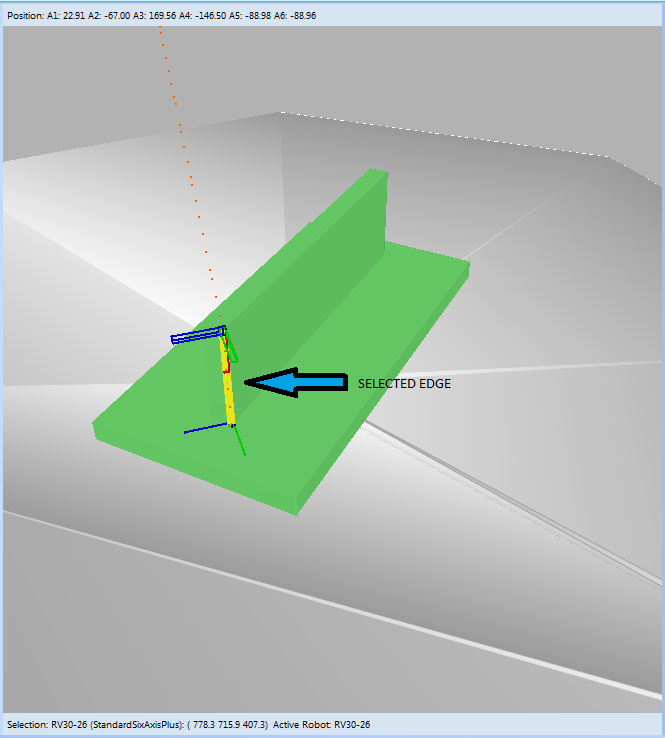
\includegraphics[width=1\textwidth,height=0.2\textheight]{images/normwp_left.png}}
		\caption{Edge to be welded}  
		\label{fig:cp2b}
	\end{subfigure}
	\begin{subfigure}[b]{0.4\textwidth}
		\frame{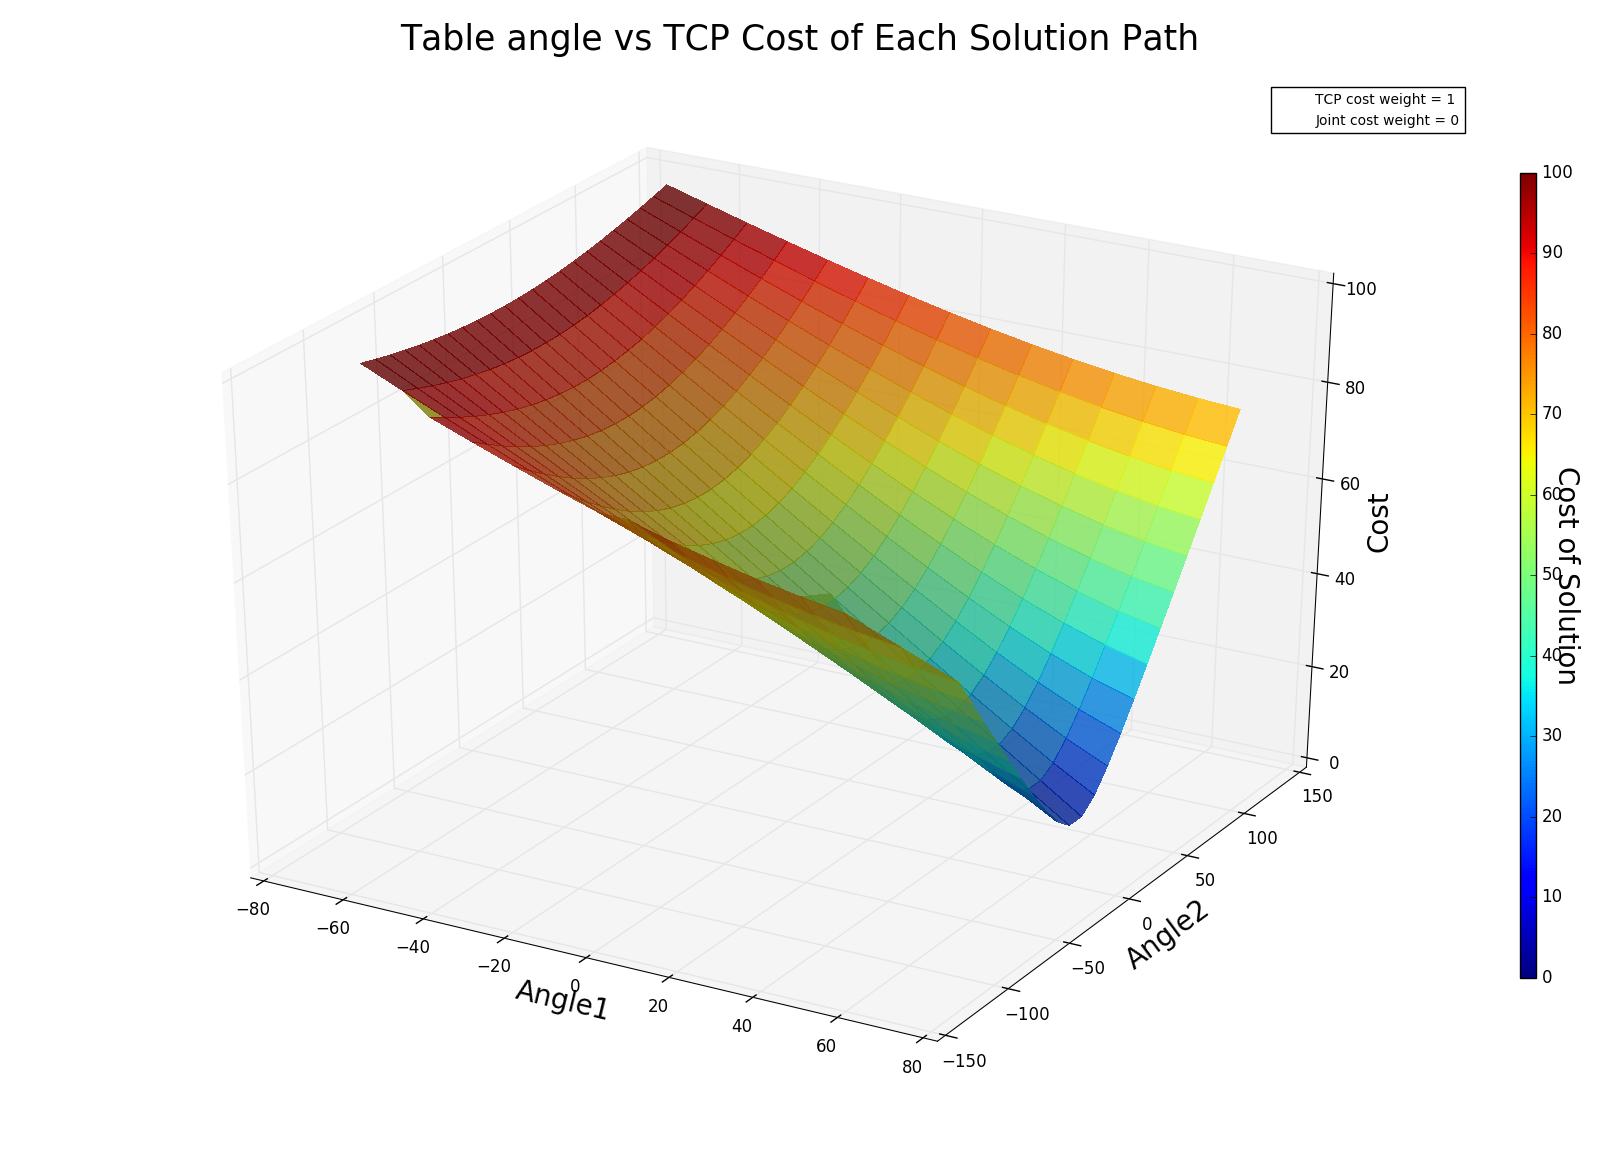
\includegraphics[width=1\textwidth,height=0.2\textheight]{images/orileft_tcpcst.png}}
		\caption{Cost Function Plot}  
		\label{fig:cp2a}
	\end{subfigure}	
	\caption{Cost Function Plot of T-Jointed workpiece: TCP orientation}
	\label{fig:cp2}
\end{figure}
The edge to be welded is marked in yellow\ref{fig:cp2b}. In the cost plot \ref{fig:cp2a}, the minimum cost is obtained when the joint angle - which moves the table along x axis - is at +80$^{\circ}$ and joint angle 2 - rotation along Z axis - is at 0$^{\circ}$.
The cost functions for the Automatica 2016 workpiece are presented below. Similar to the previous cases, the edge to be welded is marked in yellow. Red represents a higher cost gradient while blue represents a lower one. The cost value was scaled in a range of 0 to 100 to make it easier to compare the results.

\begin{figure}[!htbp] %  figure placement: here, top, bottom, or page
	\centering
	\begin{subfigure}[b]{0.4\textwidth}
		\frame{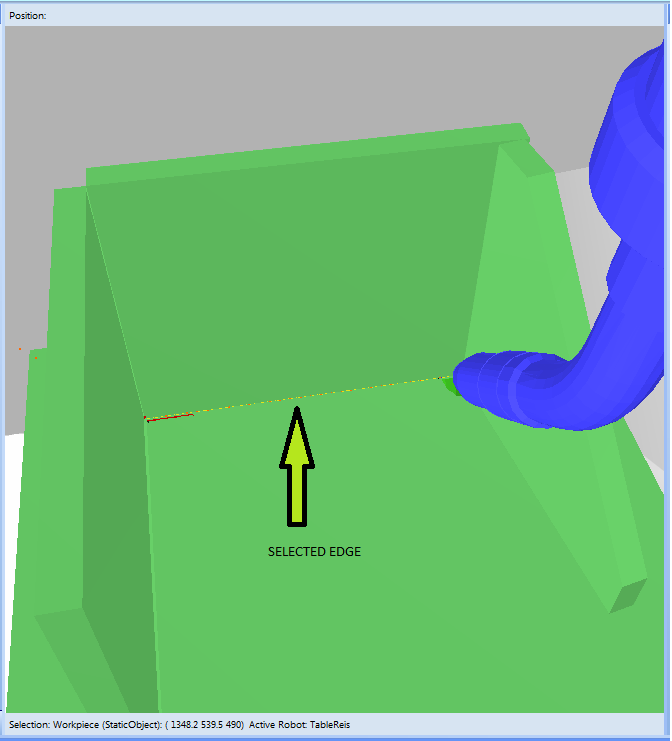
\includegraphics[width=1\textwidth,height=0.2\textheight]{images/auto_flat.png}}
		\caption{Edge to be welded}  
		\label{fig:cp3b}
	\end{subfigure}
	\begin{subfigure}[b]{0.4\textwidth}
		\frame{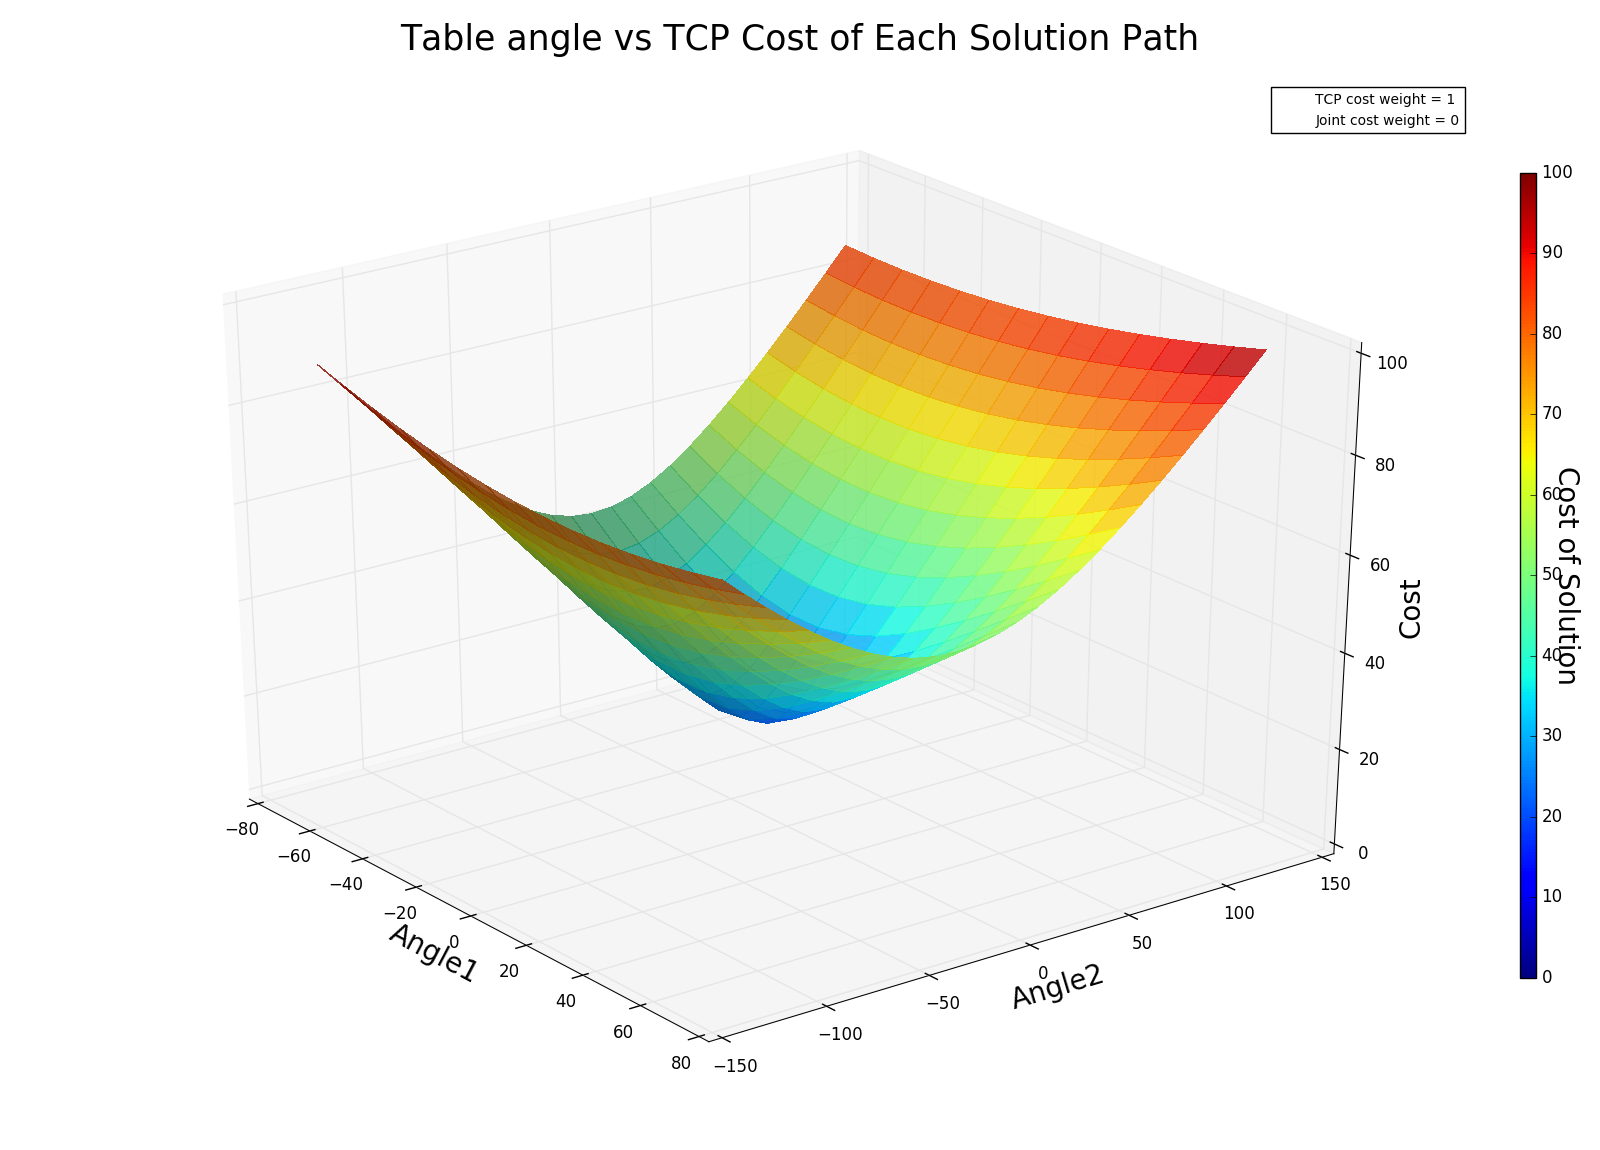
\includegraphics[width=1\textwidth,height=0.2\textheight]{images/autohori_tcpcst.png}}
		\caption{Cost Function Plot}  
		\label{fig:cp3a}
	\end{subfigure}	
	\caption{Cost Function Plot of Automatica workpiece: TCP orientation}
	\label{fig:cp3}
\end{figure}
For this particular weld task, there is a collision at both the start and end points of the weld path between the TCP and workpiece. For this reason the TCP is rotated by certain degrees at both the start and end point, which results in the minimum cost to be high compared to \ref{fig:cp1a}, even though the weld paths are quite similar. The collision scenario is illustrated in \ref{fig:coll}
\begin{figure}[!htbp] %  figure placement: here, top, bottom, or page
	\centering
	\begin{subfigure}[b]{0.4\textwidth}
		\frame{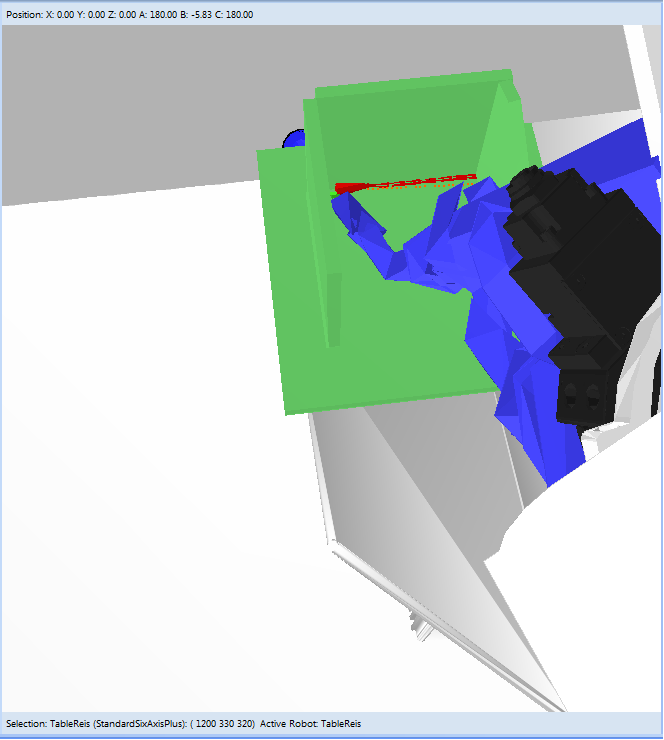
\includegraphics[width=1\textwidth,height=0.2\textheight]{images/auto_strtc.png}}
		\caption{Collision at Start Point}  
		\label{fig:colls}
	\end{subfigure}
	\begin{subfigure}[b]{0.4\textwidth}
		\frame{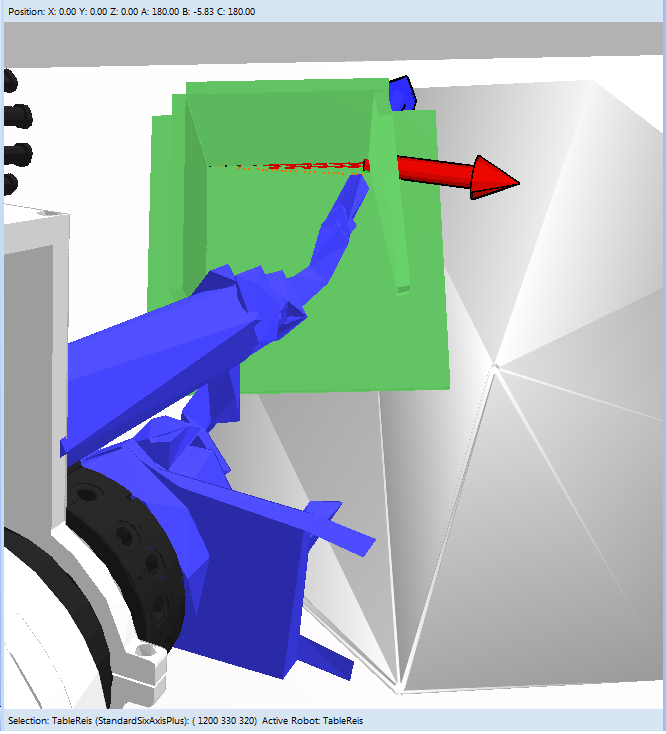
\includegraphics[width=1\textwidth,height=0.2\textheight]{images/auto_endc.png}}
		\caption{Collision at End Point}  
		\label{fig:collg}
	\end{subfigure}	
	\caption{Collision of TCP with workpiece}
	\label{fig:coll}
\end{figure}\\
For the use case in figure:\ref{fig:cp4}, the minimum cost can be observed from \ref{fig:cp4a}, to be when joint angle 1 is at 0$^{\circ}$ and joint angle 2 is at 90$^{\circ}$. Similar to the situation described in (\ref{fig:coll}), a collision at the end point of the selected edge, results in the minimum cost to become significantly high.
\begin{figure}[!htbp] %  figure placement: here, top, bottom, or page
	\centering
	\begin{subfigure}[b]{0.4\textwidth}
		\frame{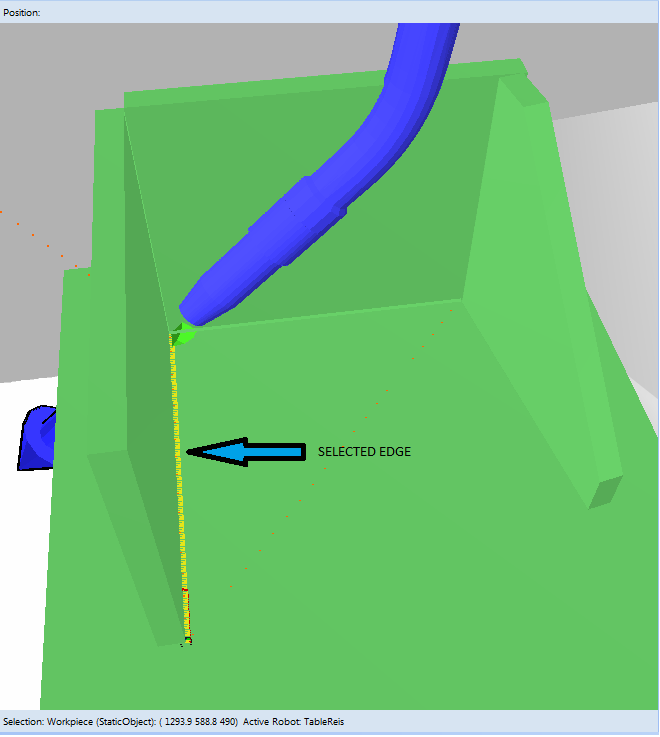
\includegraphics[width=1\textwidth,height=0.2\textheight]{images/auto_left.png}}
		\caption{Edge to be welded}  
		\label{fig:cp4b}
	\end{subfigure}
	\begin{subfigure}[b]{0.4\textwidth}
		\frame{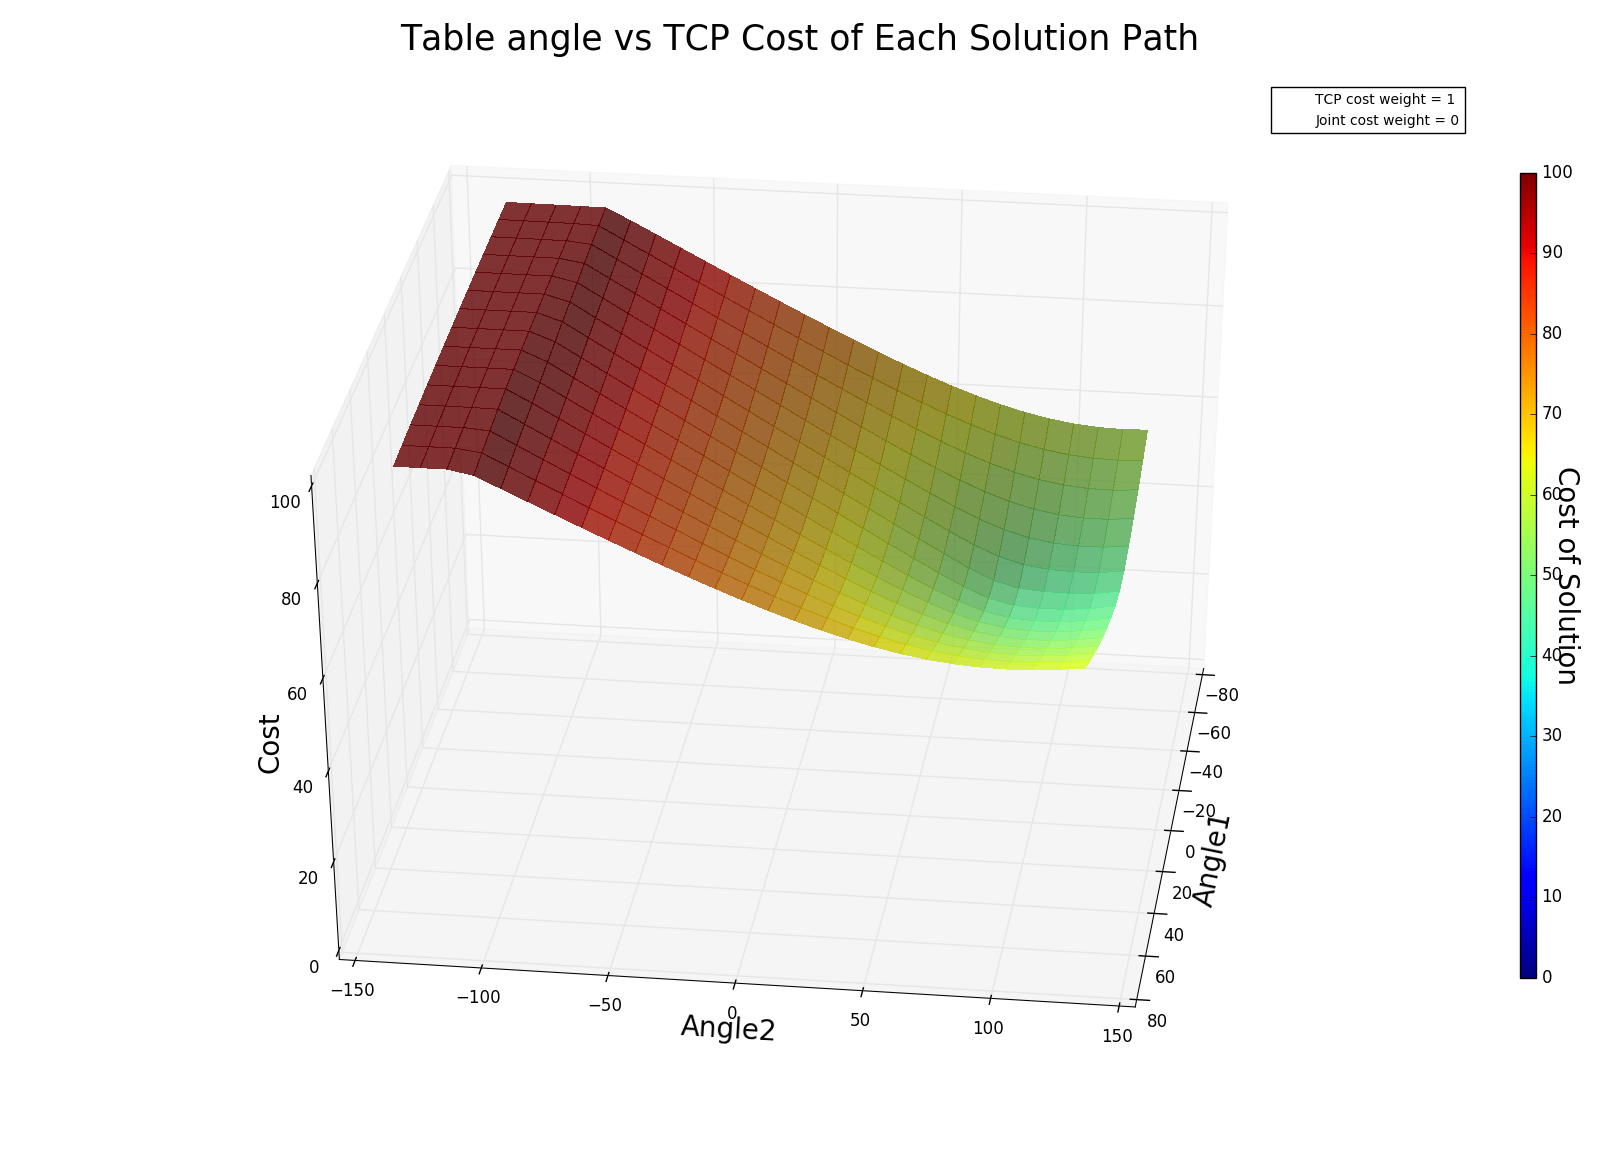
\includegraphics[width=1\textwidth,height=0.2\textheight]{images/autolft_tcpcst.png}}
		\caption{Cost Function Plot}  
		\label{fig:cp4a}
	\end{subfigure}	
	\caption{Cost Function Plot of Automatica workpiece: TCP orientation}
	\label{fig:cp4}
\end{figure}

\subsubsection{Cost Function based on Joint Movement}
\label{sssec:jntcst}
Industrial robots usually carry heavy load which makes it necessary to use high powered motors to move the bigger joints like the 1st and 2nd joints. However, usually for the smaller joints i.e. 4,5 and 6 lower powered motors are used as the load carried by these joints are lower. This concept was exploited to formulate a cost function, wherein the goal is to find weld path plans for which the movement of the bigger joints are minimal. The following table(\ref{tab3}) illustrates the power consumption of the motors of the 6 joints for the Reis Robot. 
\begin{table}[!ht]
	\centering
	\caption{Reis Robot Joint Specifications}
	\label{tab3}
	\begin{tabular}{@{}cccccc@{}}
		\toprule
		& Voltage(V) & Current(A) & Power(kW) & Torque(Nm) & RPM  \\ \midrule
		Base Joint(M1)  & 360        & 10         & 3.6       & 12         & 3800 \\
		2nd Joint(M2)   & 360        & 16.2       & 4.9       & 21.5       & 3800 \\
		3rd Joint(M3)   & 360        & 7.7        & 2.7       & 10.5       & 3800 \\
		4th Joint(M4)   & 360        & 5.1        & 1.9       & 6.2        & 3800 \\
		5th Joint(M5)   & 360        & 5.1        & 1.9       & 6.2        & 3800 \\
		Wrist Joint(M6) & 360        & 2.4        & 0.8       & 2.7        & 4000 \\ \bottomrule
	\end{tabular}
\end{table}
The first step for plotting the space, was to generate weld path solutions for every possible values of the table joint angles and record the corresponding joint angle values of robot. The joint angle values were recorded for all solution points of each weld path along with the start and goal points. Next, to calculate the cost value, we take the weighted sum of the amount of joint movement for the a particular solution path. Total joint movement is the sum of  difference of the joint angles between two consecutive solution points of a solution path. In \ref{eq23}, $C_{final}$ represents the joint cost, $w_{i}$ represents weightage value of joint \textit{i}, $\theta$ is the angle value of joint \textit{i} in degrees, \textit{k} is the solution point number and \textit{n} is the maximum number of solution points generated for a particular edge.
\begin{equation}
\label{eq23}
C_{joint}(\textit{Solution}) = \sum_{i=1}^{6}(w_{i}*\sum_{k=1}^{n}\Delta \theta_{i,k})
\end{equation}
where,
\begin{equation}
\label{eq24}
\Delta \theta_{i,k} = \theta_{i,k+1} - \theta_{i,k}
\end{equation}

The cost value was scaled in a range of 0 to 100 similar to \hyperref[sssec:tcpcst]{previous section} in order to maintain uniformity and allow us to compare the results, we will next analyze the cost functions plots.

\begin{figure}[!ht] %  figure placement: here, top, bottom, or page
	\centering
	\begin{subfigure}[b]{0.4\textwidth}
		\frame{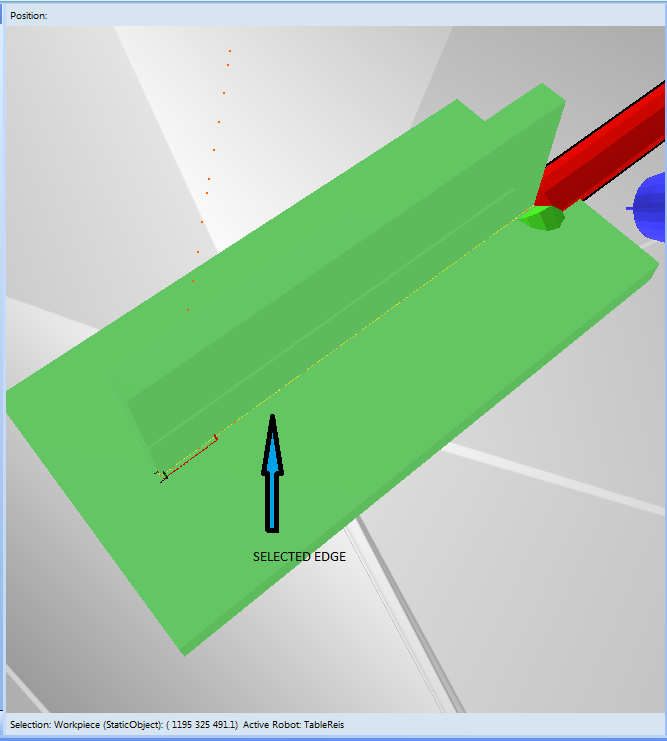
\includegraphics[width=1\textwidth,height=0.2\textheight]{images/normwp_flat.png}}
		\caption{Edge to be welded}  
		\label{fig:17a}
	\end{subfigure}
	\begin{subfigure}[b]{0.4\textwidth}
		\frame{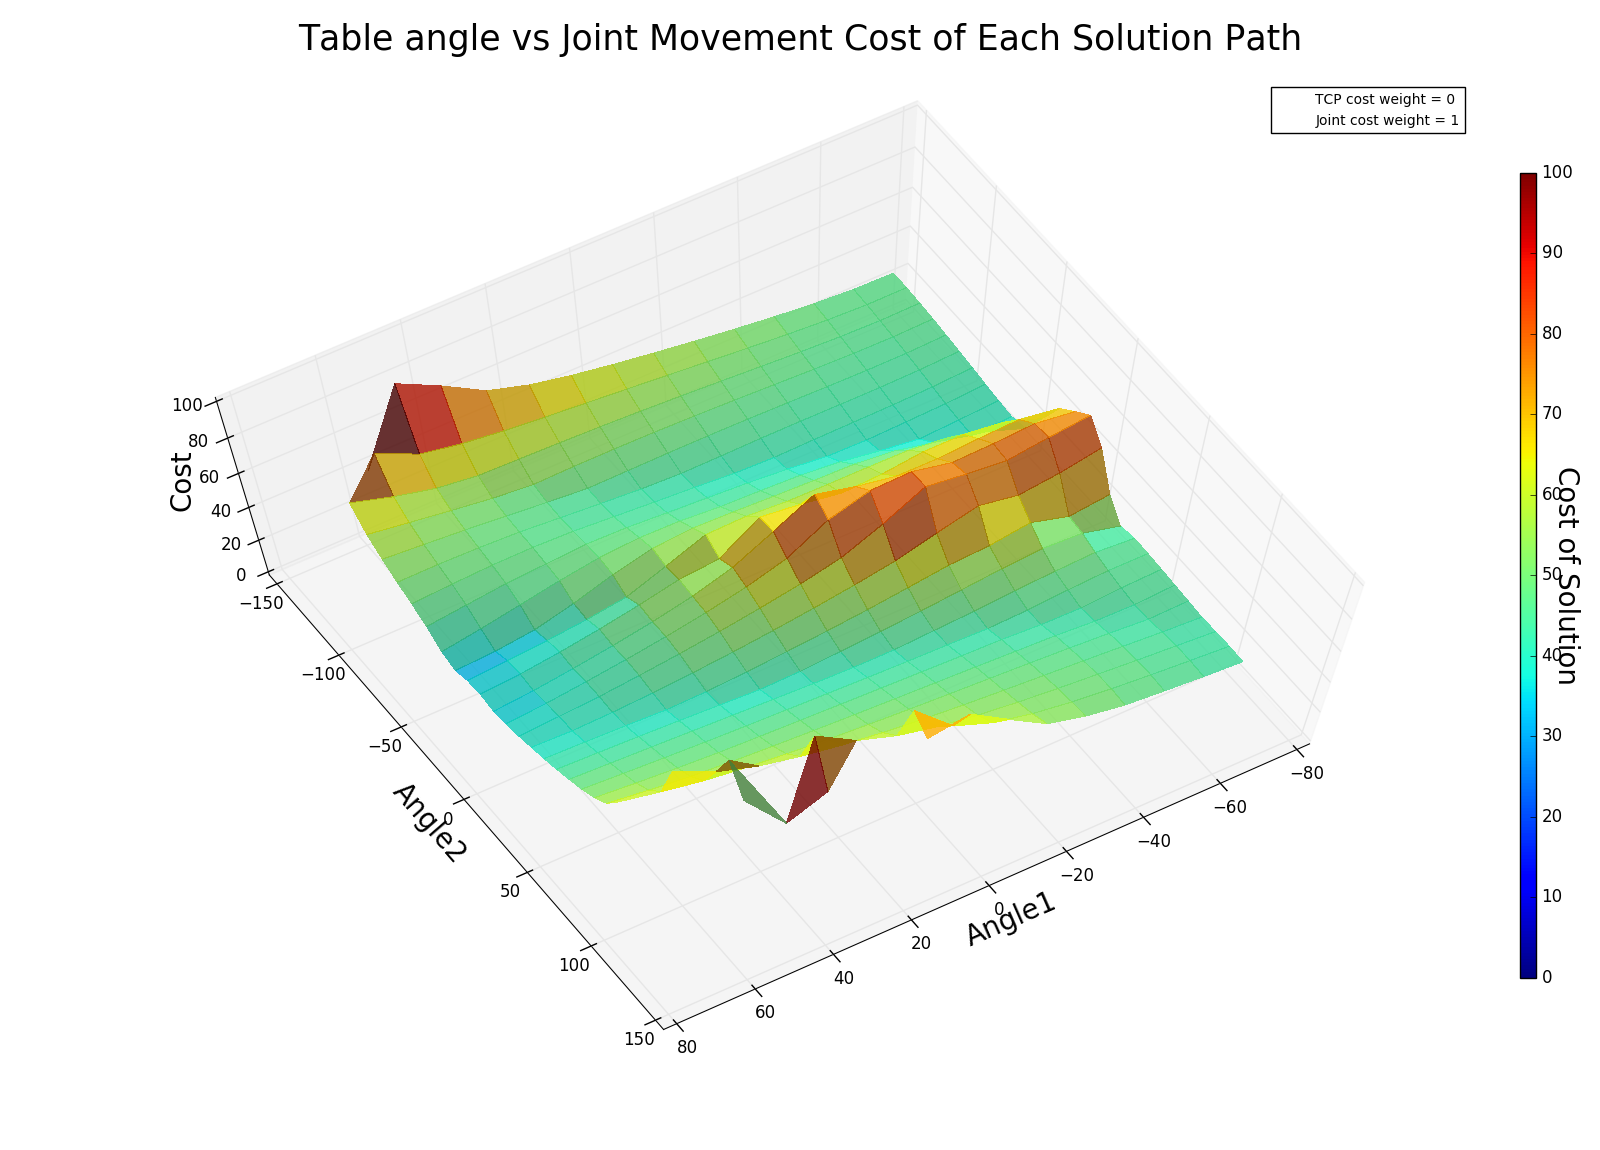
\includegraphics[width=1\textwidth,height=0.2\textheight]{images/orihori_jntcst.png}}
		\caption{Cost Function Plot}  
		\label{fig:17b}
	\end{subfigure}	
	\begin{subfigure}[b]{0.4\textwidth}
		\frame{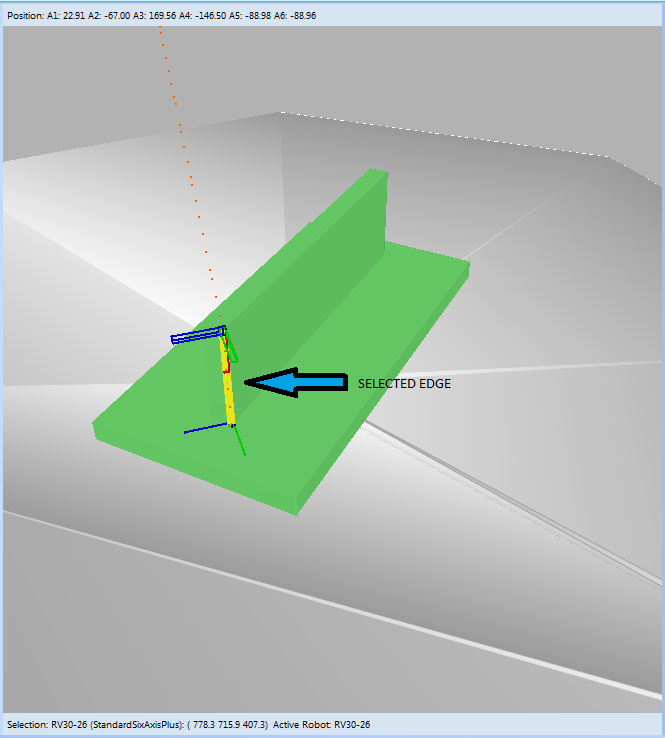
\includegraphics[width=1\textwidth,height=0.2\textheight]{images/normwp_left.png}}
		\caption{Edge to be welded}  
		\label{fig:17c}
	\end{subfigure}
	\begin{subfigure}[b]{0.4\textwidth}
		\frame{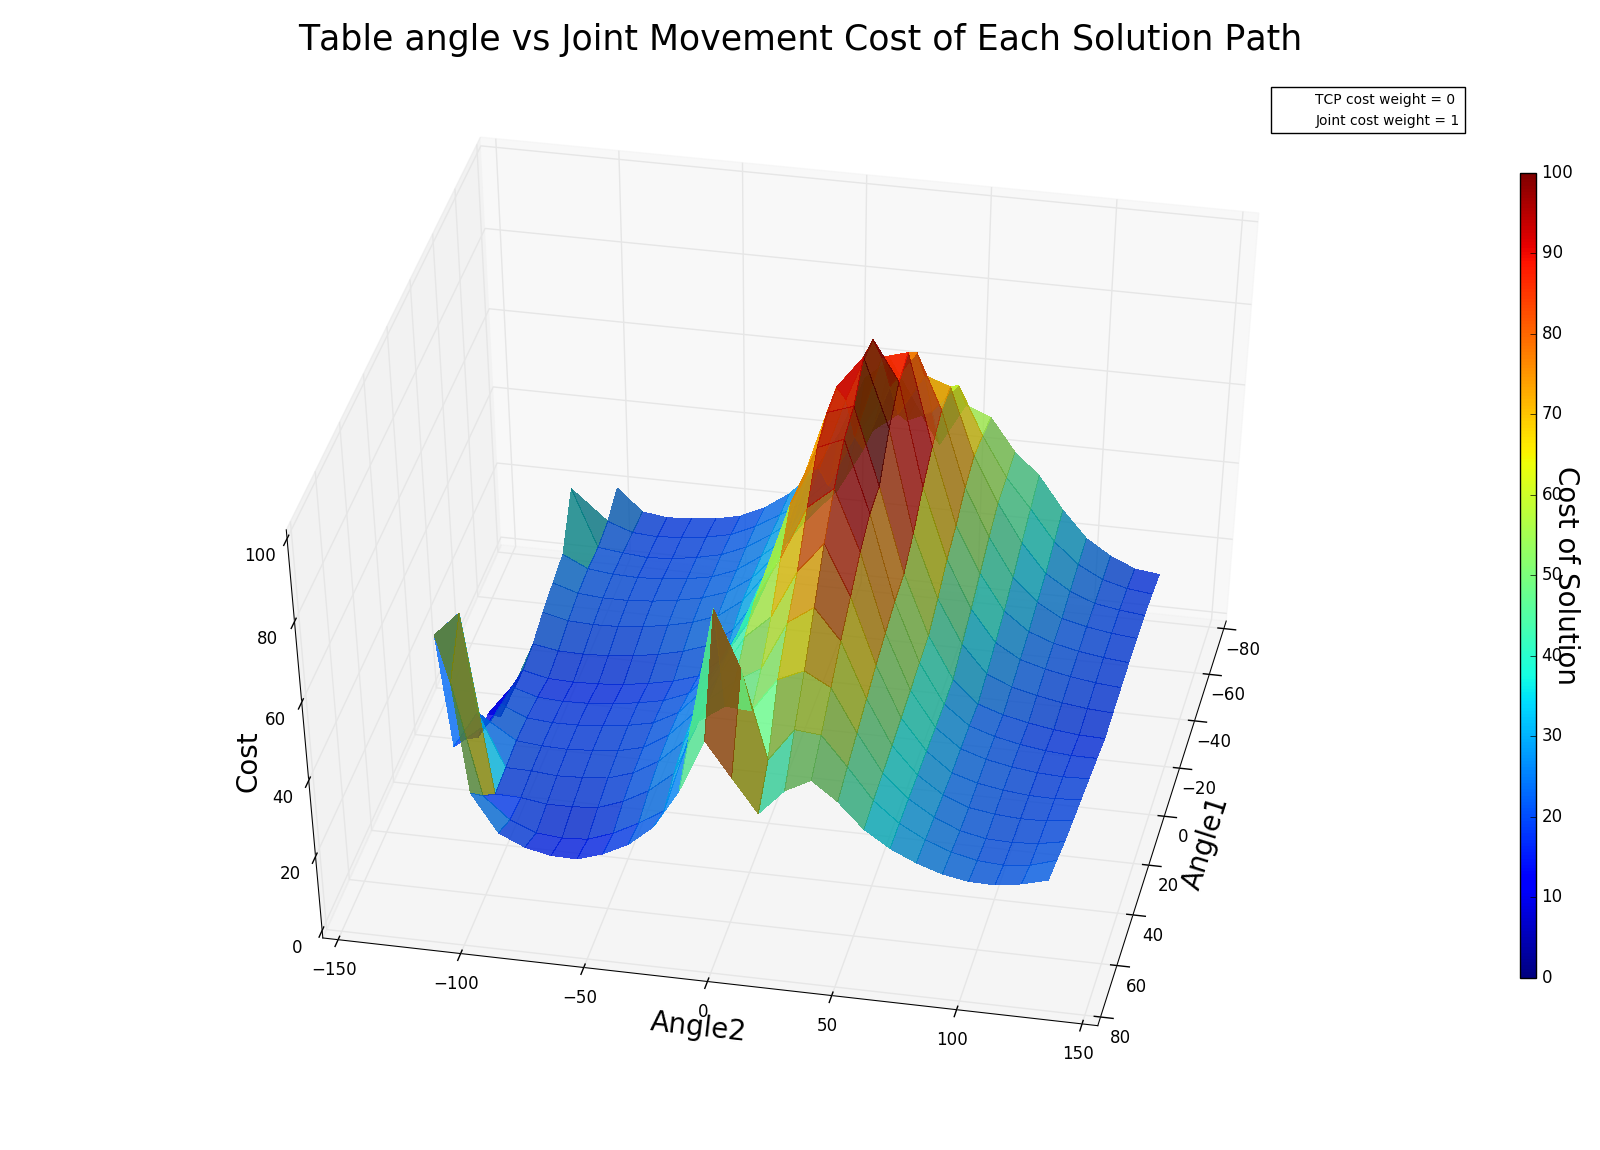
\includegraphics[width=1\textwidth,height=0.2\textheight]{images/orileft_jntcst2.png}}
		\caption{Cost Function Plot}  
		\label{fig:17d}
	\end{subfigure}	
	\caption{Cost Function Plot of T-Jointed workpiece: Joint Movement}
	\label{fig:17}
\end{figure}

From the plots (\ref{fig:17b}) \& (\ref{fig:17d}) of both the use cases, we can interpret that for the T-jointed workpiece, when both the joint angles of the table are at 0$^{\circ}$, the cost is the highest, which means for the weld paths at these positions of the table, the bigger joints move the most. While rotating  joint angle2 of the table has the most significant effect on generating solutions with lower cost. 
\clearpage

\begin{figure}[!ht] %  figure placement: here, top, bottom, or page
	\centering
	\begin{subfigure}[b]{0.4\textwidth}
		\frame{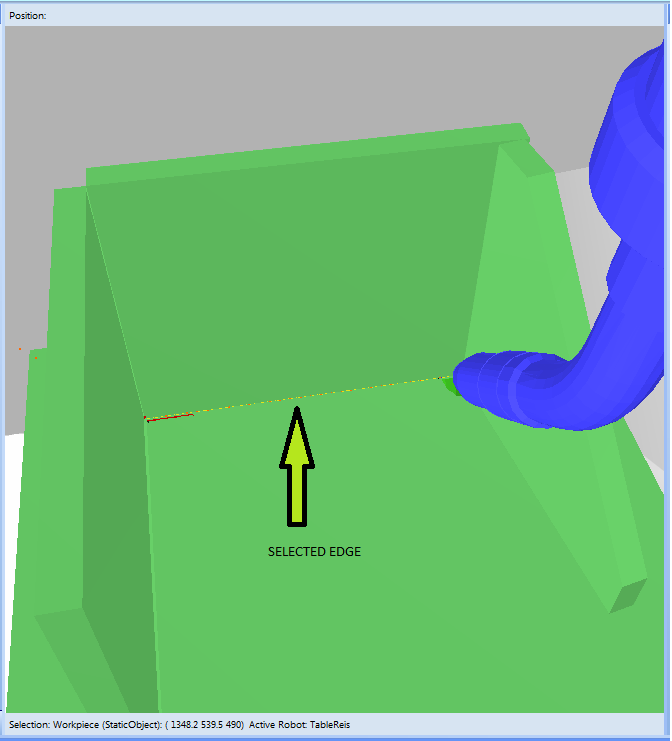
\includegraphics[width=1\textwidth,height=0.2\textheight]{images/auto_flat.png}}
		\caption{Edge to be welded}  
		\label{fig:18a}
	\end{subfigure}
	\begin{subfigure}[b]{0.4\textwidth}
		\frame{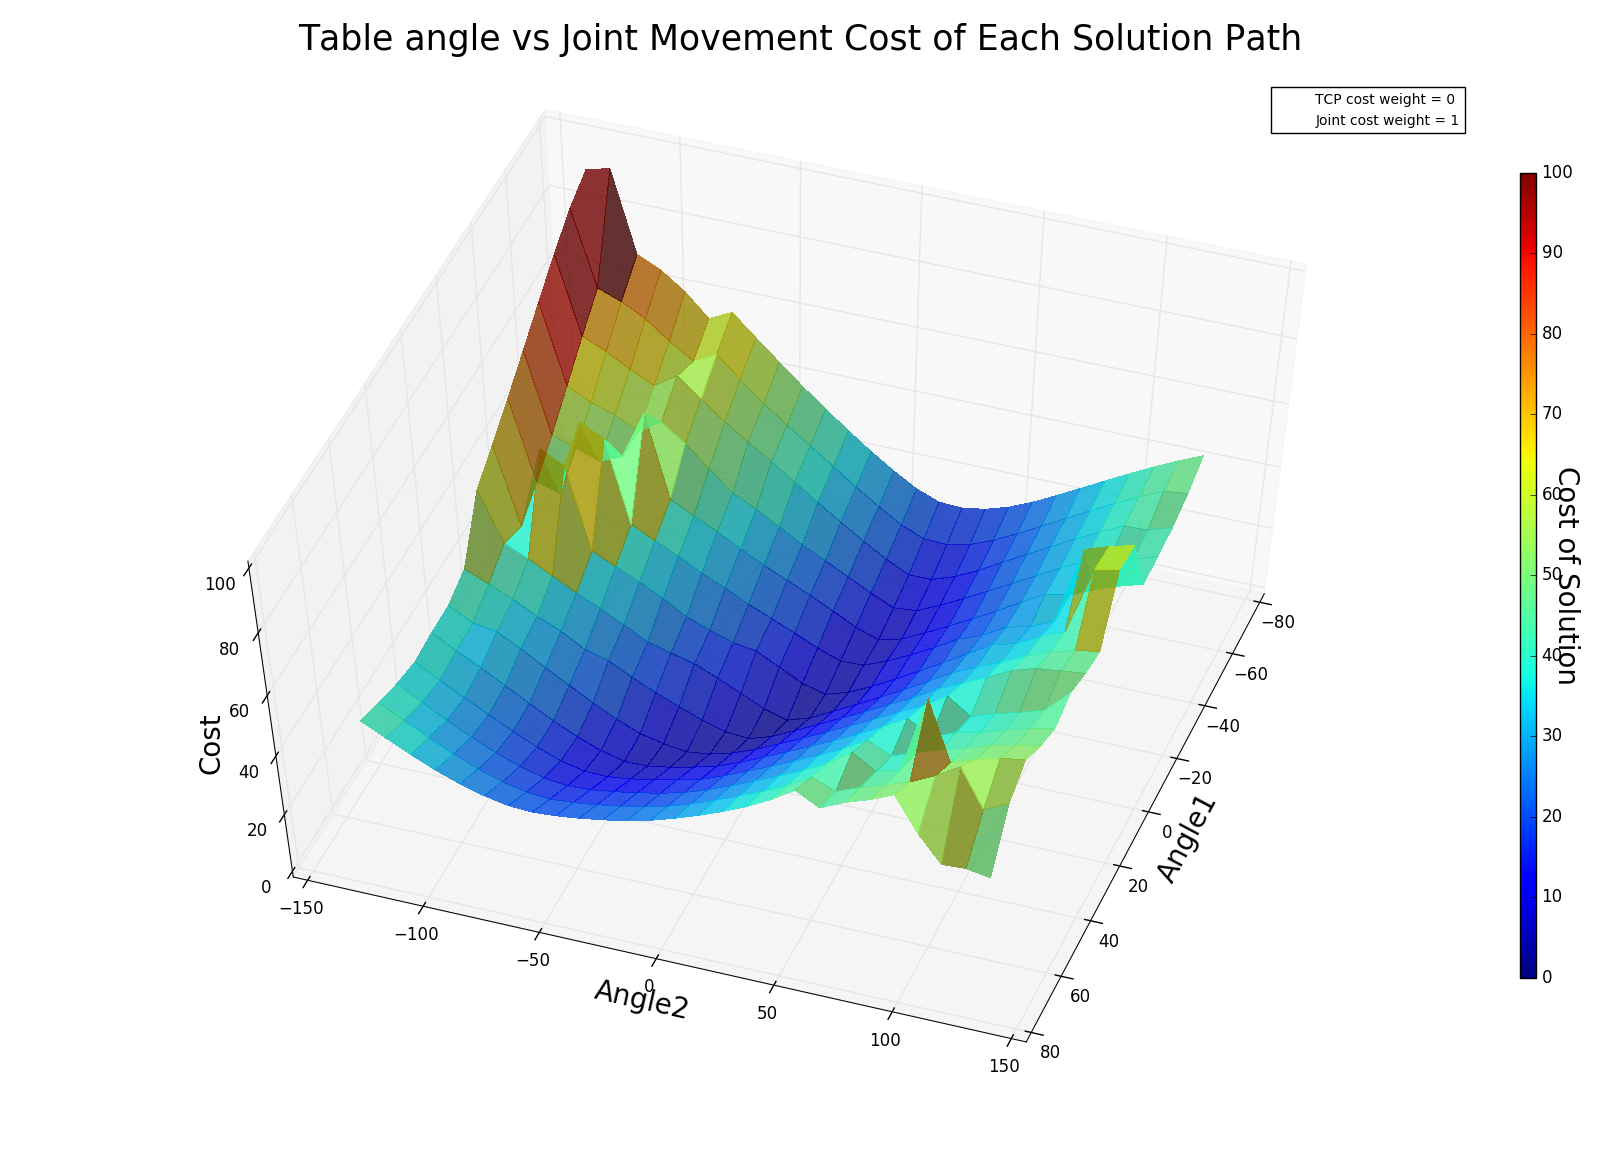
\includegraphics[width=1\textwidth,height=0.2\textheight]{images/autohori_jntcst.png}}
		\caption{Cost Function Plot}  
		\label{fig:18b}
	\end{subfigure}	
	\begin{subfigure}[b]{0.4\textwidth}
		\frame{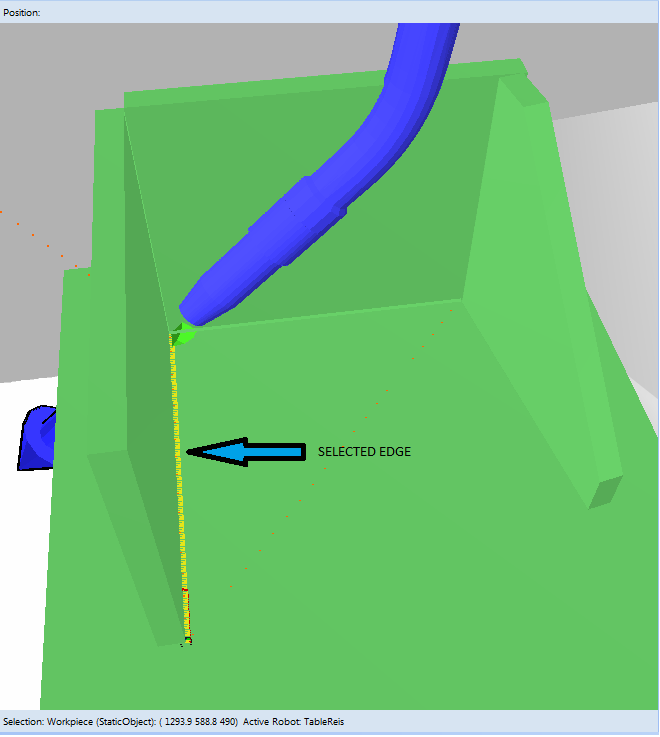
\includegraphics[width=1\textwidth,height=0.2\textheight]{images/auto_left.png}}
		\caption{Edge to be welded}  
		\label{fig:18c}
	\end{subfigure}
	\begin{subfigure}[b]{0.4\textwidth}
		\frame{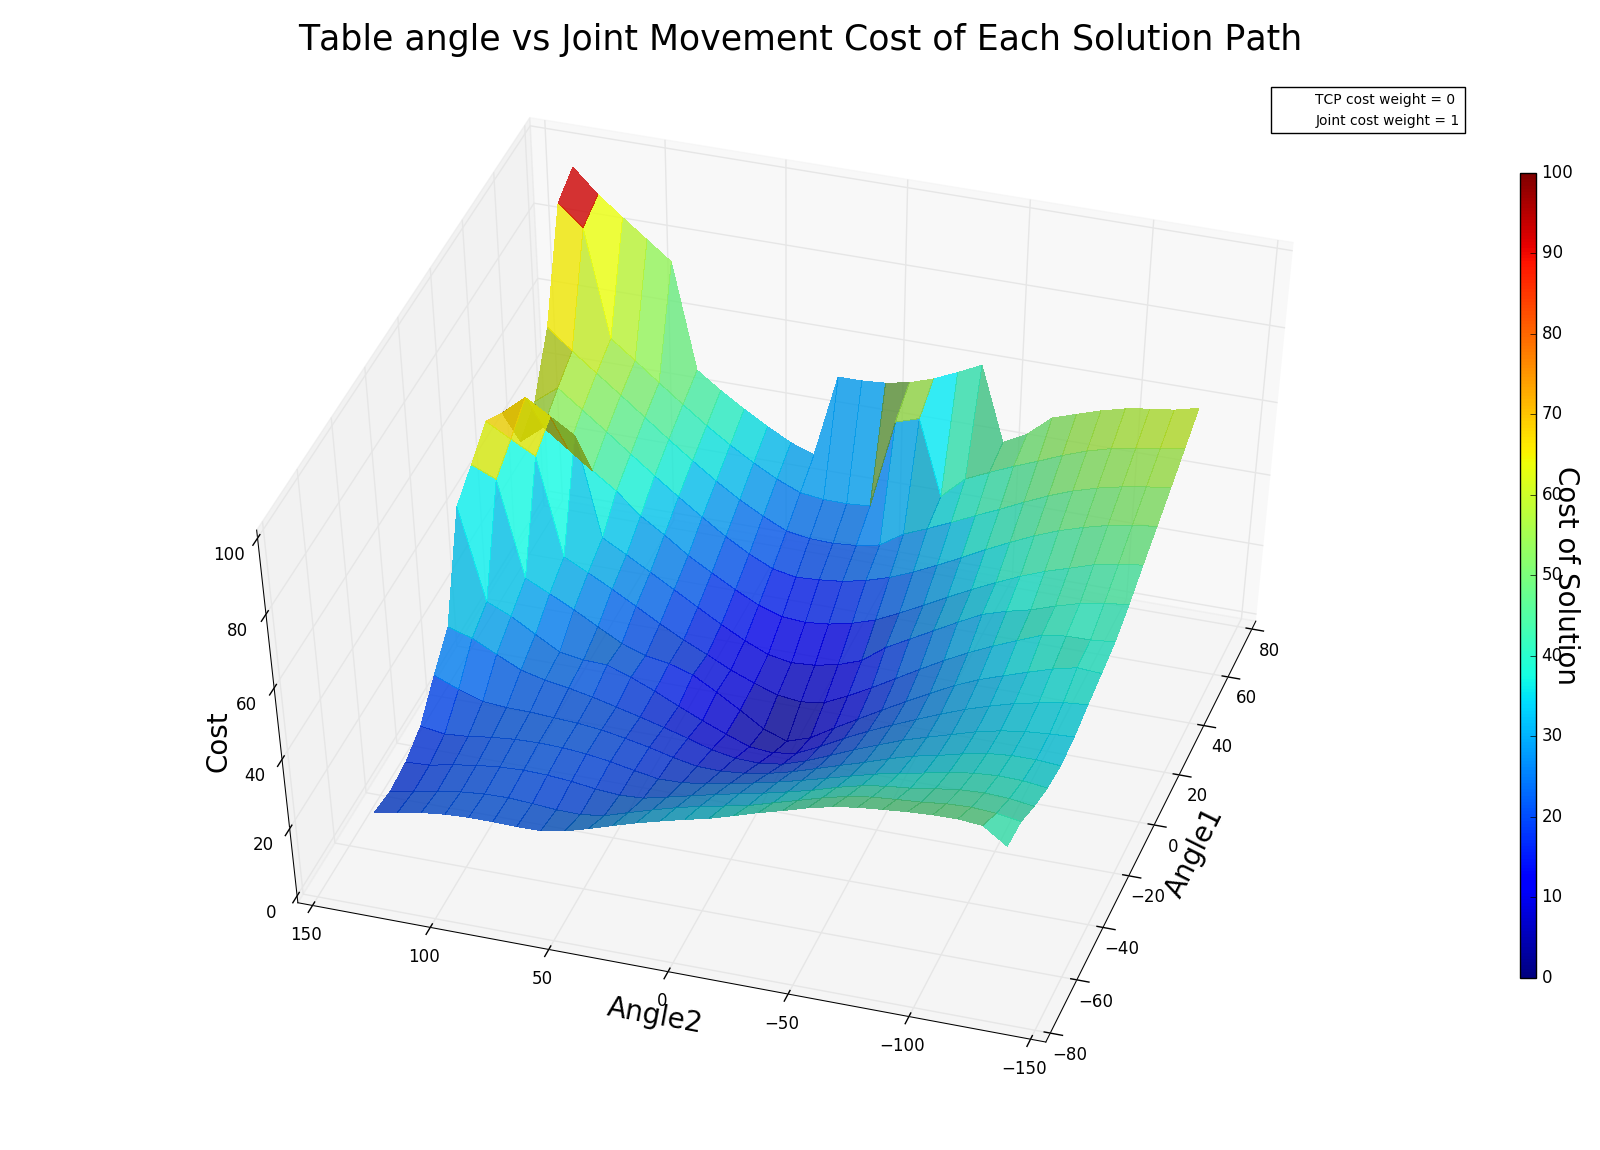
\includegraphics[width=1\textwidth,height=0.2\textheight]{images/autolft_jntcst.png}}
		\caption{Cost Function Plot}  
		\label{fig:18d}
	\end{subfigure}	
	\caption{Cost Function Plot of Automatica workpiece: Joint Movement}
	\label{fig:18}
\end{figure}

From the plots (\ref{fig:18b}) \& (\ref{fig:18d}) of both the use cases, we can interpret that for the Automatica workpiece, when both the joint angles of the table are at 0$^{\circ}$, the cost is the lowest, which means for the weld paths at these positions of the table, the bigger joints move the least, which is completely different from what we observed in (\ref{fig:17}). 

\subsubsection{Cumulative Cost Function}
\label{sssec:aggcst}
Based on the cost functions defined in sections (\ref{sssec:tcpcst}) and (\ref{sssec:jntcst}), the cumulative cost function is formulated. The concept behind this cost function is that, based on the welding task and the environment in which it is to be performed we can decide which aspect of welding is more important. For e.g in cases where generating perfect welds are critical to the structural integrity of the end product, we can assign a greater weightage to the TCP orientation cost, as it is directly linked with the quality of weld based on process description as stated in [\citet{DiazP2016}]. However a situation might also arise where consuming lesser power - while generating a weld path - is more relevant for e.g while prototyping an user will weld on a workpiece multiple times in which case his/her main priority would be minimize the power consumption instead of generating a perfect weld. The mathematical formulation of the cumulative cost function is presented in \ref{eq25}, where $C_{agg}$ is the cumulative sum, $w_{tcp}$ and $w_{joint}$ are the weights assigned to TCP and joint costs respectively and $C_{tcp}$ and $C_{joint}$ are the TCP and joint costs respectively. 
\begin{equation}
\label{eq25}
C_{agg}(\textit{Solution}) = w_{tcp}* C_{tcp} +  w_{joint}*C_{joint}
\end{equation}
Cumulative cost function plots for both use cases \hyperref[fig:uc1]{1} and \hyperref[fig:uc2]{2} were generated with the following weights: 
\begin{itemize}
\item TCP cost weightage:0.2, Joint cost weightage:0.8 
\item TCP cost weightage:0.4, Joint cost weightage:0.6
\item TCP cost weightage:0.5, Joint cost weightage:0.5
\item TCP cost weightage:0.6, Joint cost weightage:0.2
\end{itemize}

\begin{figure}[!ht] %  figure placement: here, top, bottom, or page
	\centering
		\frame{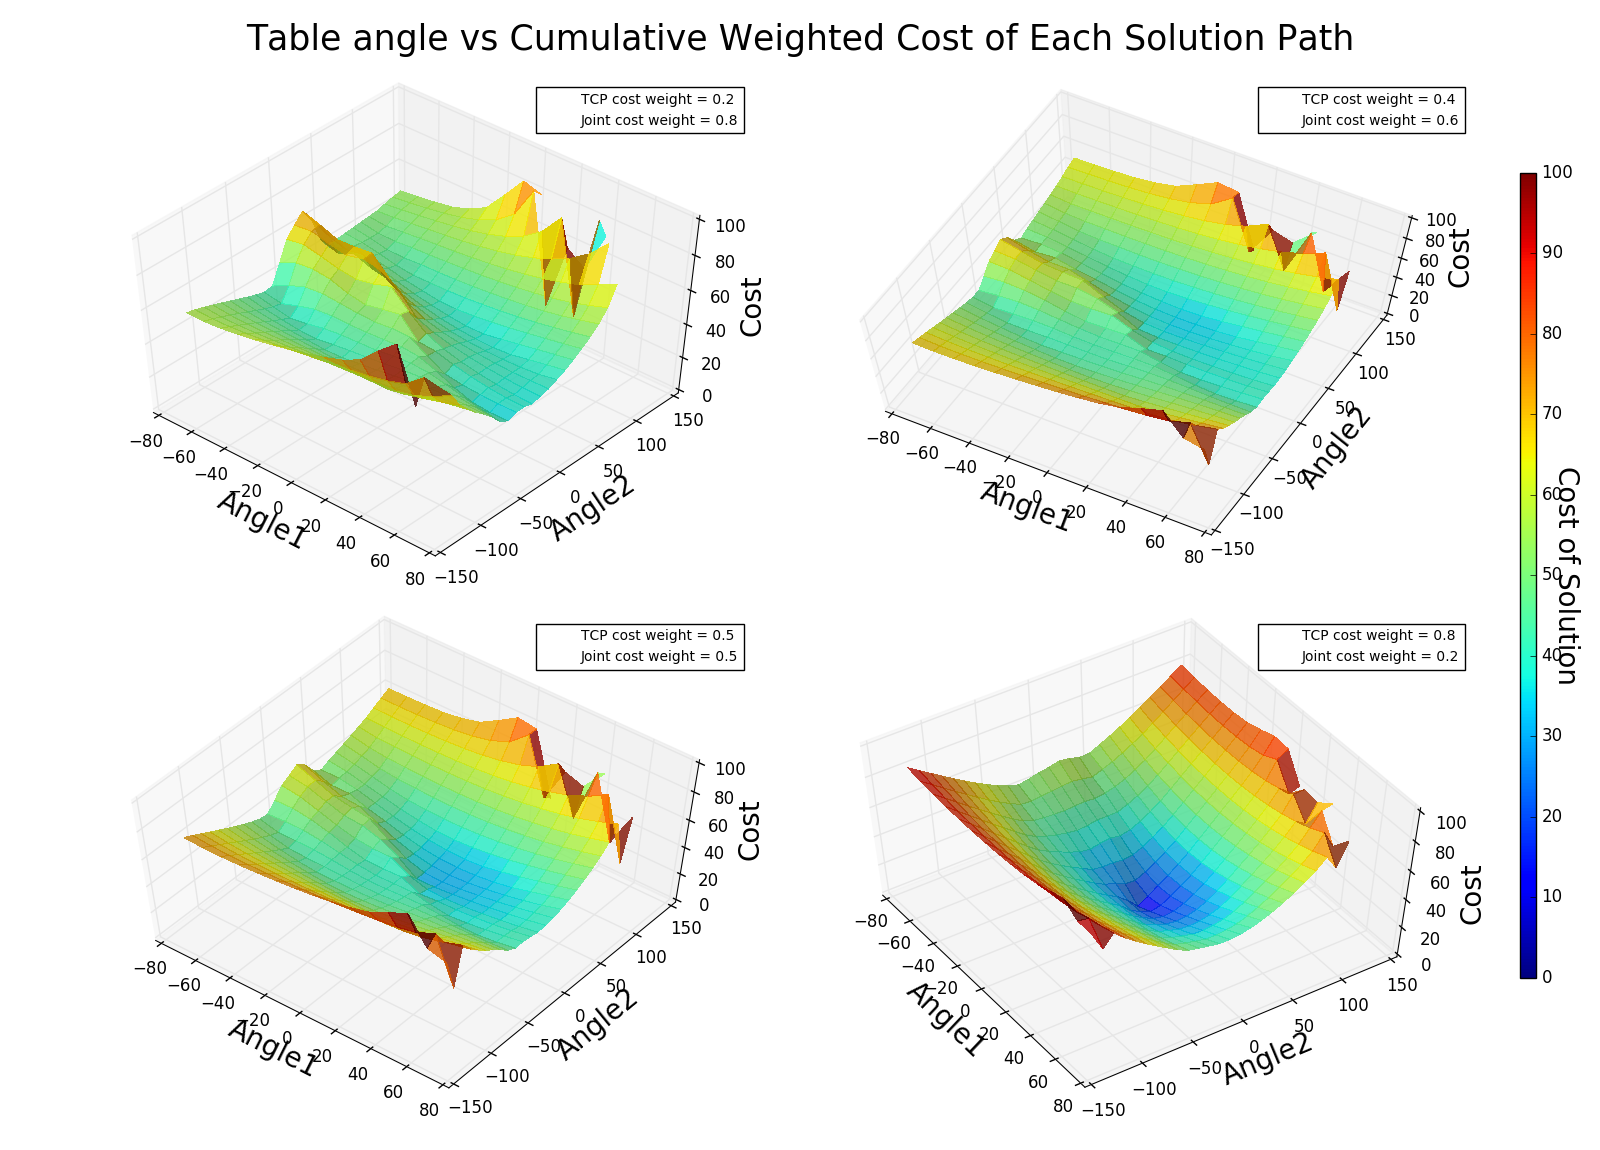
\includegraphics[width=1\textwidth]{images/orihori_totcst.png}}
		\caption{Cumulative Cost Function for T-Jointed Workpiece Horizontal Edge(\ref{fig:imguc1})}
		\label{fig:tot1}
\end{figure}
In plot \ref{fig:tot1}, we can observe that when the weightage values are both 0.5, a common area (marked by blue colored region), can be observed where the minimum cost of both the functions, overlap. For the other plots, the function with the higher weightage determines the shape of the plot, which is in accordance with our earlier results in sections (\ref{sssec:tcpcst}) and (\ref{sssec:jntcst})

\begin{figure}[!ht] %  figure placement: here, top, bottom, or page
	\centering
	\frame{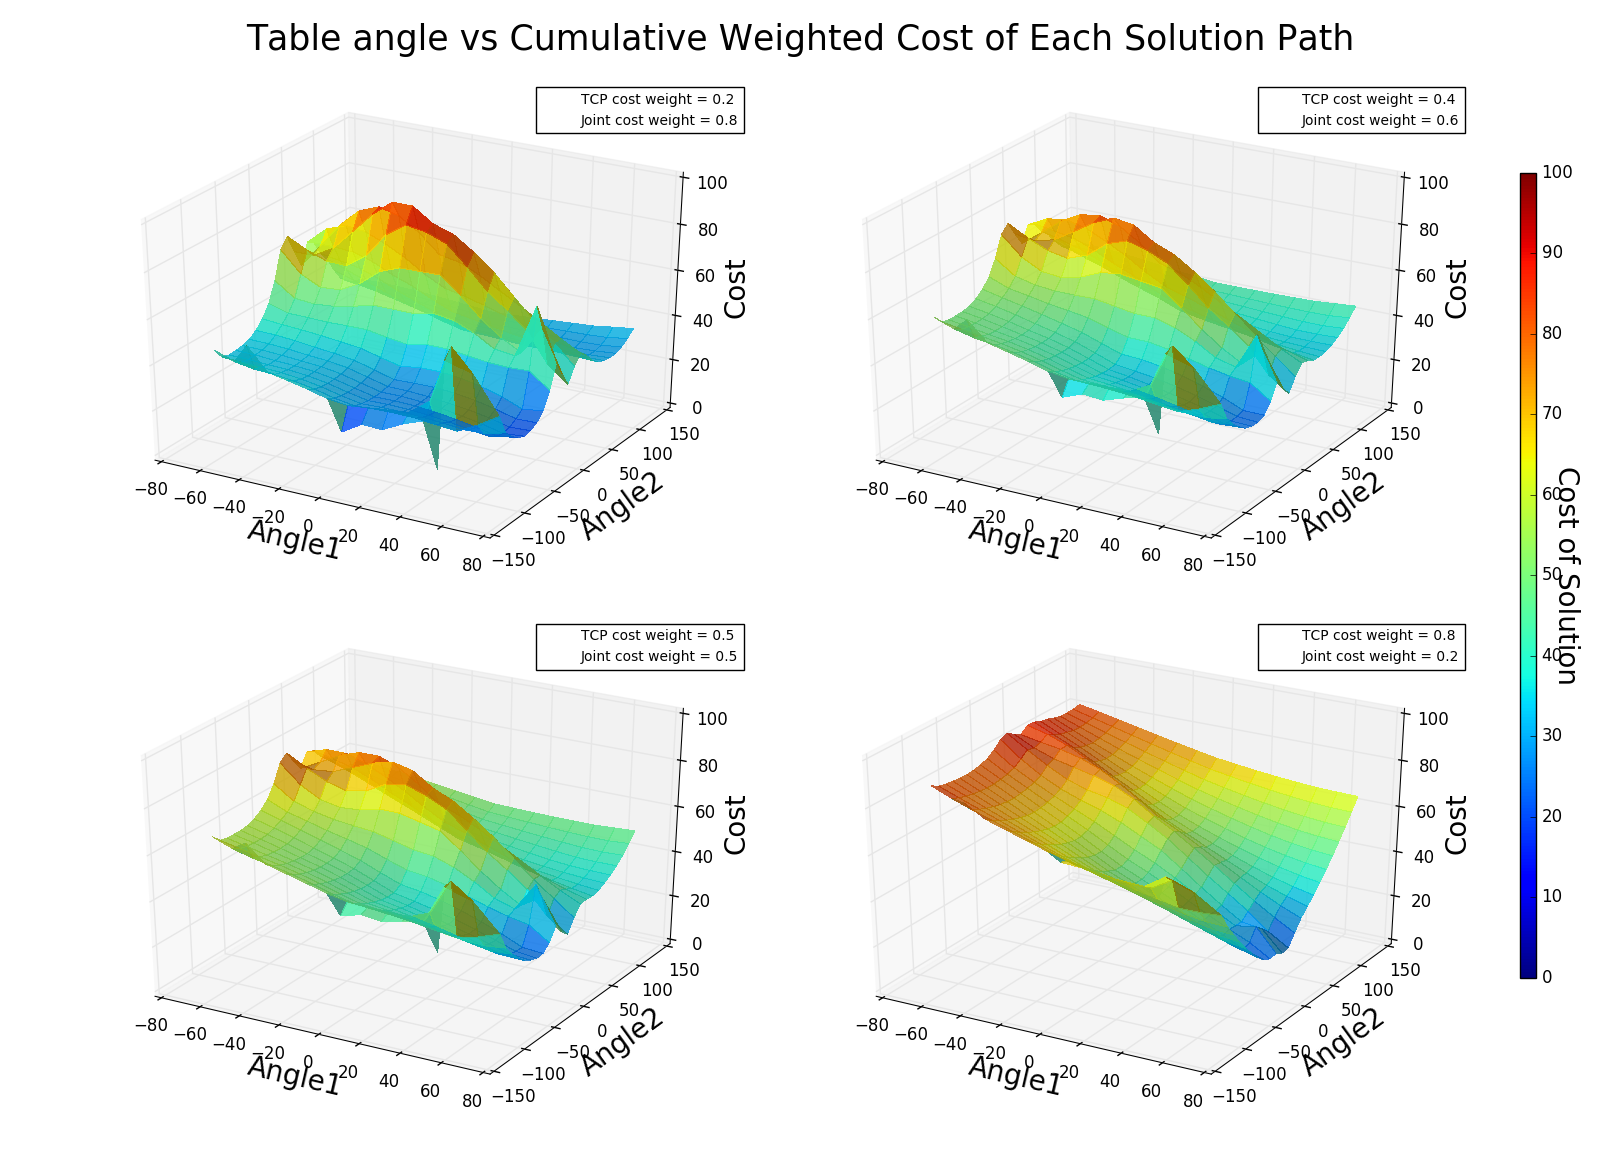
\includegraphics[width=1\textwidth]{images/orileft_totcst.png}}
	\caption{Cumulative Cost Function for T-Jointed Workpiece Vertical Edge(\ref{fig:imguc2})}
	\label{fig:tot2}
\end{figure}
Similarly in plot \ref{fig:tot2} we observe that, when the functions have equal weightage, a clear demarcation (marked by blue color) emerges. As in the previous case, the shape and features of the plot changes based on the weightage of the two functions. 

Next the plots for the \hyperref[fig:uc2]{2nd} use case are presented. 
\begin{figure}[!ht] %  figure placement: here, top, bottom, or page
	\centering
	\frame{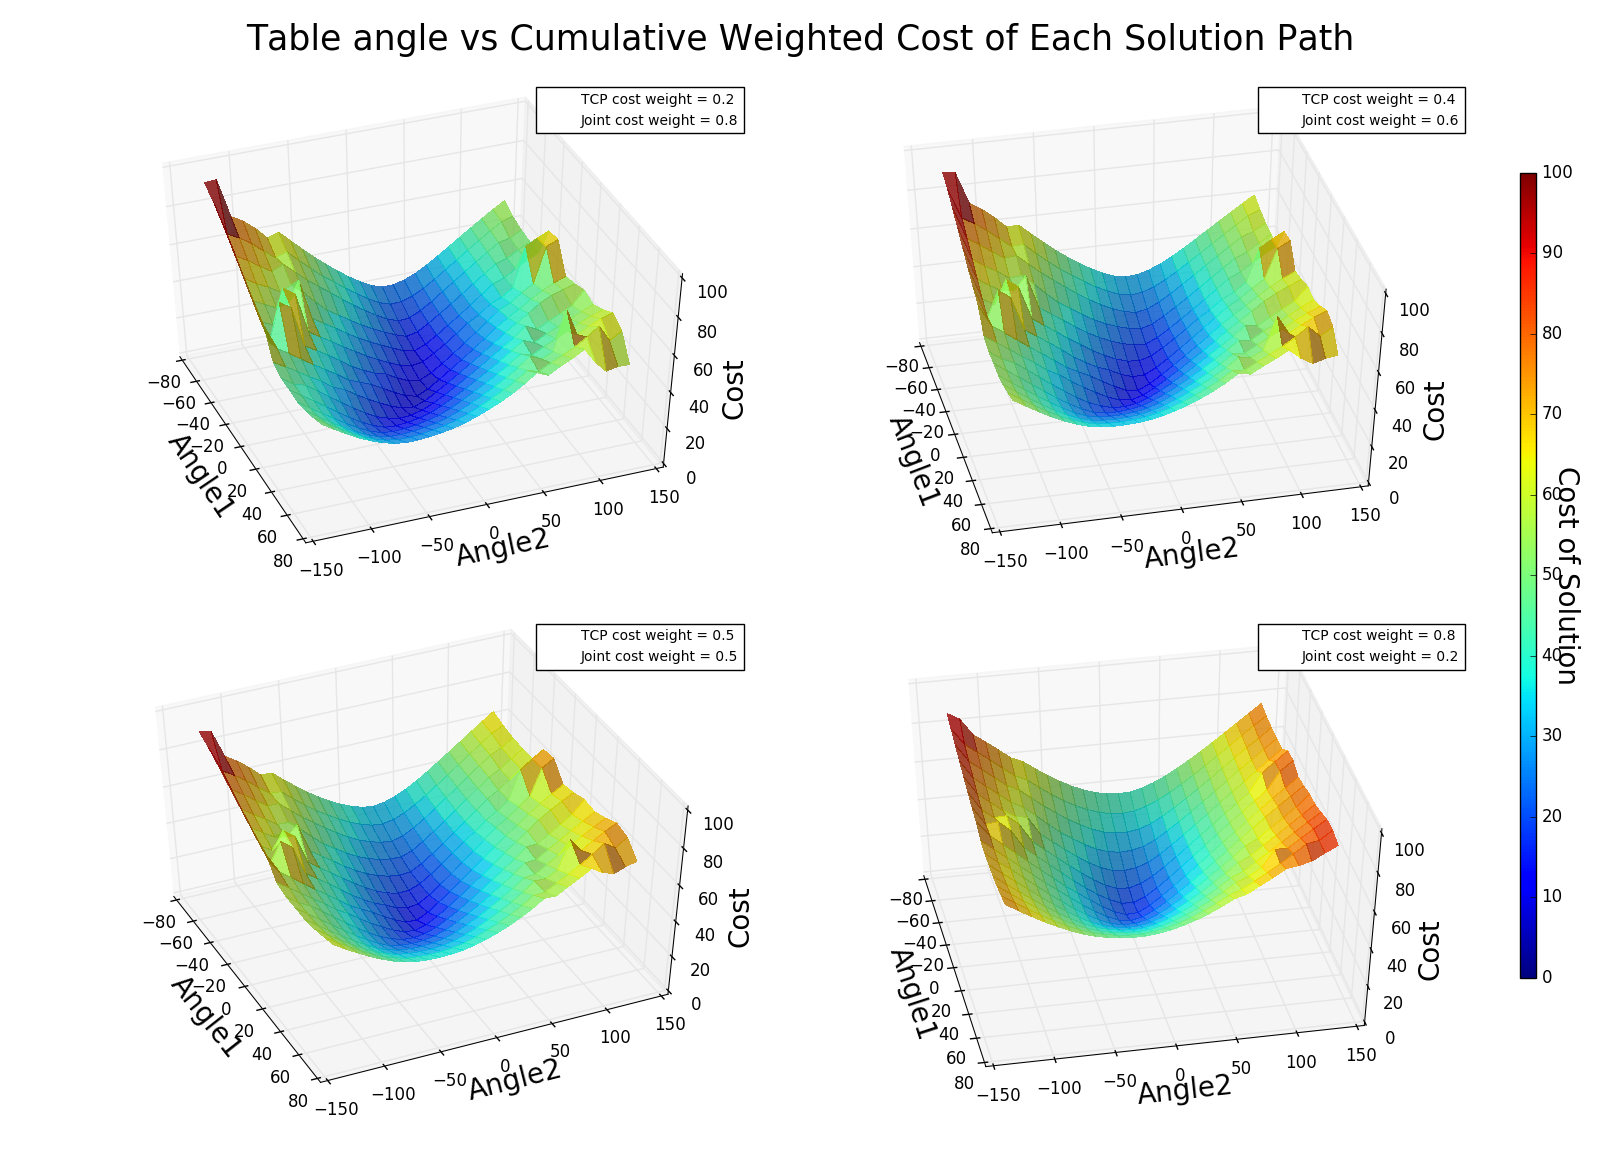
\includegraphics[width=0.8\textwidth,scale=0.6]{images/autohori_totcst.png}}
	\caption{Cumulative Cost Function for Automatica Workpiece Horizontal Edge(\ref{fig:imguc3})}
	\label{fig:tot3}
\end{figure}
Similarly in plot \ref{fig:tot3}, we can observe that when the weightage values are both 0.5, a common area (marked by blue colored region), can be observed where the minimum cost of both the functions, overlap. However for plot \ref{fig:tot4}, due to the fact the TCP cost for this use case is so high, it increases the overall minimum cost for the case when both the weightage values are 0.5. 

\begin{figure}[!ht] %  figure placement: here, top, bottom, or page
	\centering
	\frame{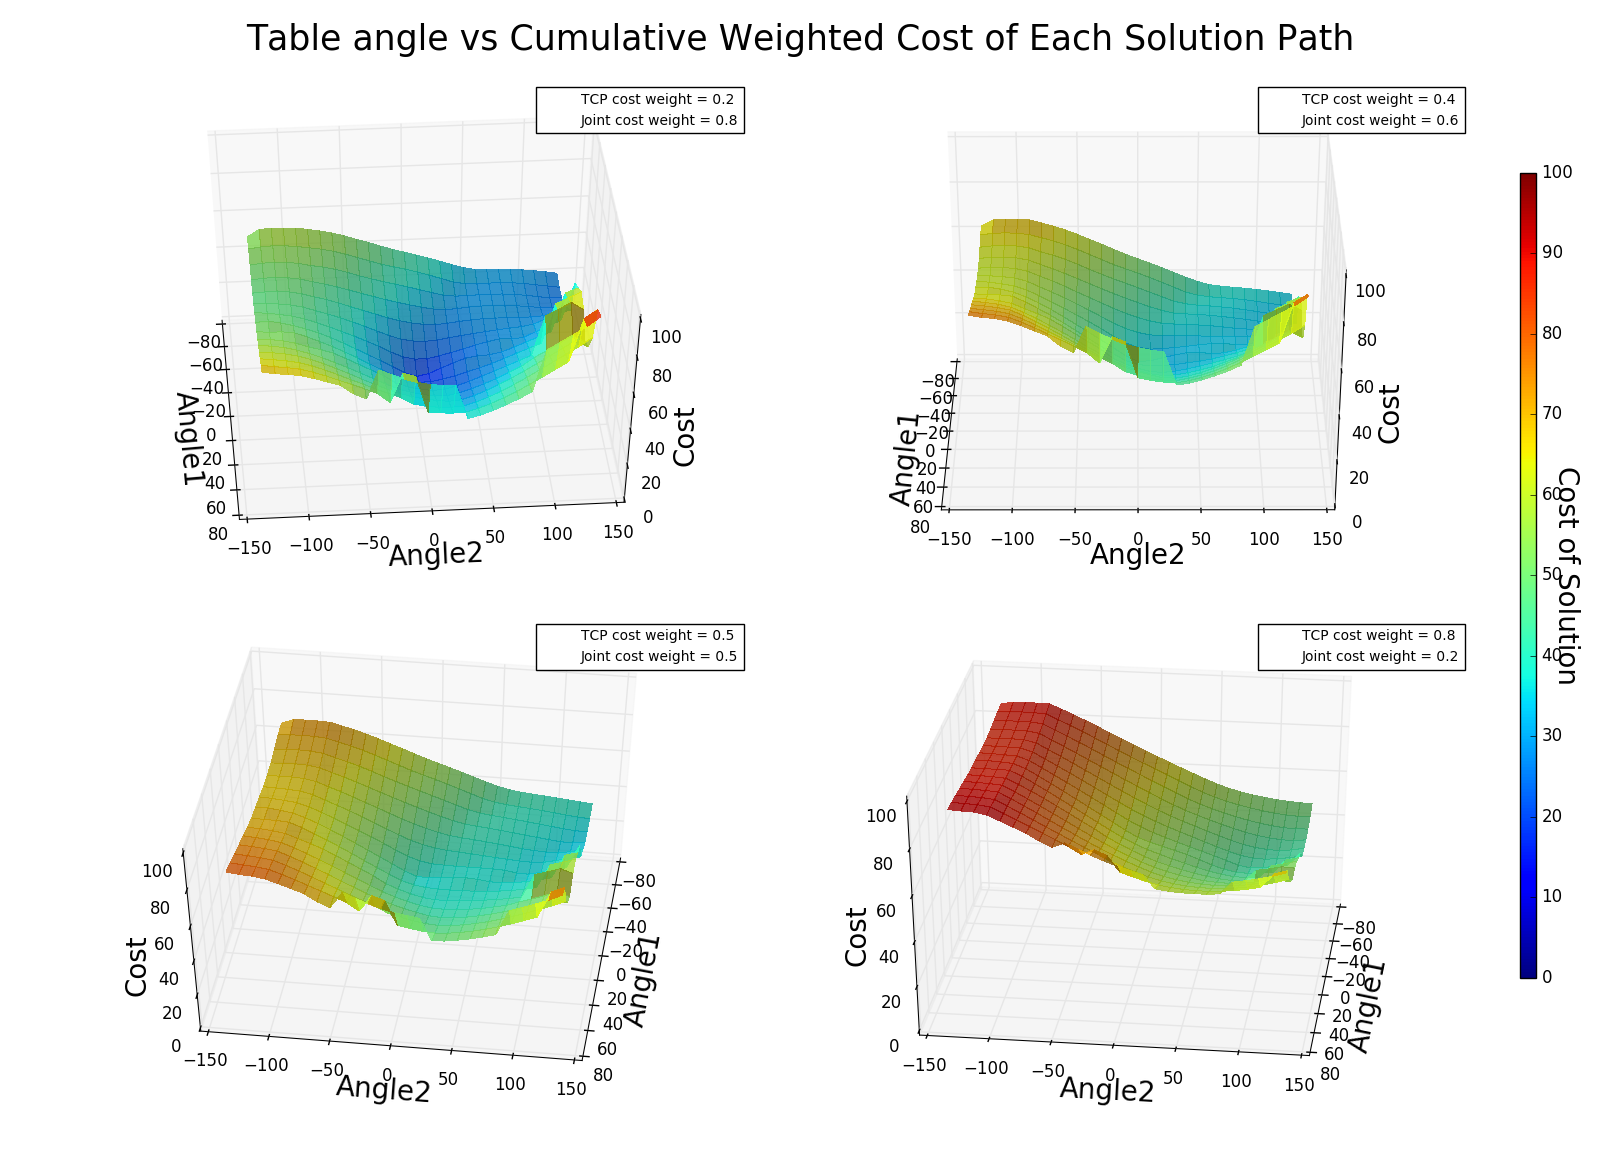
\includegraphics[width=0.8\textwidth,scale=0.6]{images/autolft_totcst.png}}
	\caption{Cumulative Cost Function for Automatica Left Horizontal Edge(\ref{fig:imguc4})}
	\label{fig:tot4}
\end{figure}
\clearpage

\subsection{Optimization Approaches}
(To determine min val)
In section \ref{ssec:cst} we plotted the cost functions for two use cases \ref{fig:uc1} and \ref{fig:uc2} and with the help of the plots we were able to determine for which values of the table joints, we can obtain weld paths with minimum cost. Even though this approach enables the user to see the cost space and make it very easy to select the optimal joint angles of the table, there are certain drawbacks to it:
\begin{itemize}
	\item The optimal cost value changes for every use case based on the workpiece, the edge to be selected and weightage of the TCP and joint cost functions.
	\item The difference in shape of the plots indicate, that it is also difficult to predict the cost values of a weld path just from the table angles, unless the solution is explicitly generated. 
	\item The inability to predict cost value coupled with the fact that the cost space is unique for different use cases, means that we have to generate plots for the entire range of the joint angles of the table for every welding use case.
	\item The generation of weld paths for every possible orientation of the table takes approximately 1 hour, which makes this process both tedious and inefficient. 
\end{itemize}
From the remarks, we can conclude that the problem at hand is a NP-hard problem, therefore the only possible way to find or approximate the optimal position would be to apply search based techniques. We consider two well known search algorithms - (i) Hill Climbing and (ii) Simulated Annealing - to find the optimum solution. While there are a plethora of other search based technique in use, for e.g Genetic/Evolutionary Algorithm - Hill Climbing or Simulated Annealing offer a perfect balance between finding the optimum and convergence time.
\subsubsection{Hill Descent Algorithm Approach}
\label{sssechd}
Hill Climbing or in our problem case, Hill Descent is a simple optimization technique which attempts to find new state from its  current state by evaluating a cost function[\citet{russell2009artificial}]. Hill descent is based on a greedy approach, i.e. it only considers the subsequent state if it is locally optimal or in other words, if the cost value of the subsequent state is lower compared to the current state. Since it does not store the previous state values, it is extremely memory efficient and fast, which make it an ideal choice for our use case. A key consideration for the algorithm to function properly - in the use case at hand - is to determine the exit criteria. The simple reason being, because the global optimum value cannot be pre-determined, we can neither specify the exit criteria as a difference of current and next solution state nor can we fix the number of iterations, as in both the cases it might lead to a suboptimal solution. Since hill descent algorithm does not use any data structure to store already explored states, the following simple solution has been devised. 
\begin{itemize}
	\item Selection of new neighbors using Manhattan/Taxicab Distance (\citet{Frnkranz2011}).
	\item This limits the number of possible neighbors to 8 for each state, since the we have a 2D space. 
	\item Following the above two conditions, we can assume that if for a certain state, all of its neighbors have higher cost values, that state can be considered as an optimum and the algorithm is terminated.
\end{itemize}

\algdef{SE}[DOWHILE]{Do}{doWhile}{\algorithmicdo}[1]{\algorithmicwhile\ #1}%
	
\begin{algorithm}
	\caption{Hill Descent Approach Based Optimal Weld Path Generation}
	\label{algo4}
	\textbf{Given:} $ \text{Initial table joint angle values \textit{$A1$} \& \textit{$A2$}}$ \\ 
	\textbf{Output:} $ \text{Table joint values for plan path generation with minimum cost}$ \\
	
	\begin{algorithmic}[1]
		\State $\text{Apply kinematic equation \ref{eq22} and set table position using \textit{$A1$} \& \textit{$A2$}}$
		\State $\text{Apply Workpiece Transformation Algorithm(\ref{algo2})}$
		\State $\text{Apply Selected Edge Transformation Algorithm(\ref{algo3})}$
		\State $\text{Perform Motion Planning on the transformed plan path and get \textit{Solution}}$
		\State $\text{\textit{CurrentCost} $\gets$ $C_{agg}$(\textit{Solution}) using equation\ref{eq25}}$
		\State $\text{(\textit{$A1_{curr}$},\textit{$A2_{curr}$}) $\gets$ (\textit{$A1$}, \textit{$A2$})}$
		\Do
		\State $\text{(\textit{$A1_{new}$},\textit{$A2_{new}$})}$ $\gets$ $\text{\textit{SelectNeighbor}(\textit{$A1_{curr}$},\textit{$A2_{curr}$},\textit{stepsize})}$
		\State $\text{Apply steps \textit{1-4} with (\textit{$A1_{new}$},\textit{$A2_{new}$})}$
		\State $\text{\textit{Stepcost} $\gets$ $C_{agg}$(\textit{Solution}) \ref{eq25}}$
		\State $\text{\textit{diff} $\gets$ \textit{Stepcost} - \textit{CurrentCost}}$
		\If {[${diff < 0}$]}
		\State $\text{\textit{PossibleMinimaCounter} $\gets$ 0}$
		\State $\text{(\textit{$A1_{curr}$},\textit{$A2_{curr}$}) $\gets$ (\textit{$A1_{new}$}, \textit{$A2_{new}$})}$
		\State $\text{\textit{CurrentCost} $\gets$ \textit{Stepcost}}$
		\Else
		\State $\text{increase \textit{PossibleMinimaCounter} by 1}$
		\EndIf  
		
		\doWhile{$\textit{PossibleMinimaCounter}$ $\leq$ 8}
		\State $\textit{return}$ ($\textit{$A1_{curr}$}$,$\textit{$A2_{curr}$}$)     
	\end{algorithmic}
\end{algorithm}
In algorithm \ref{algo4}, we randomly choose a new neighbor, using Manhattan Distance and if the new state has a lower cost, then it moves to the new state and the \textit{PossibleMinimaCounter} is set to zero. If however, the new neighbor has a higher cost value, then the \textit{PossibleMinimaCounter} is incremented by 1. If the value of \textit{PossibleMinimaCounter} reaches 8, then we consider that state as a minimum state and exit the algorithm. Following this, we execute the algorithm and plot the results.
\begin{figure}[!ht] %  figure placement: here, top, bottom, or page
	\centering
	\frame{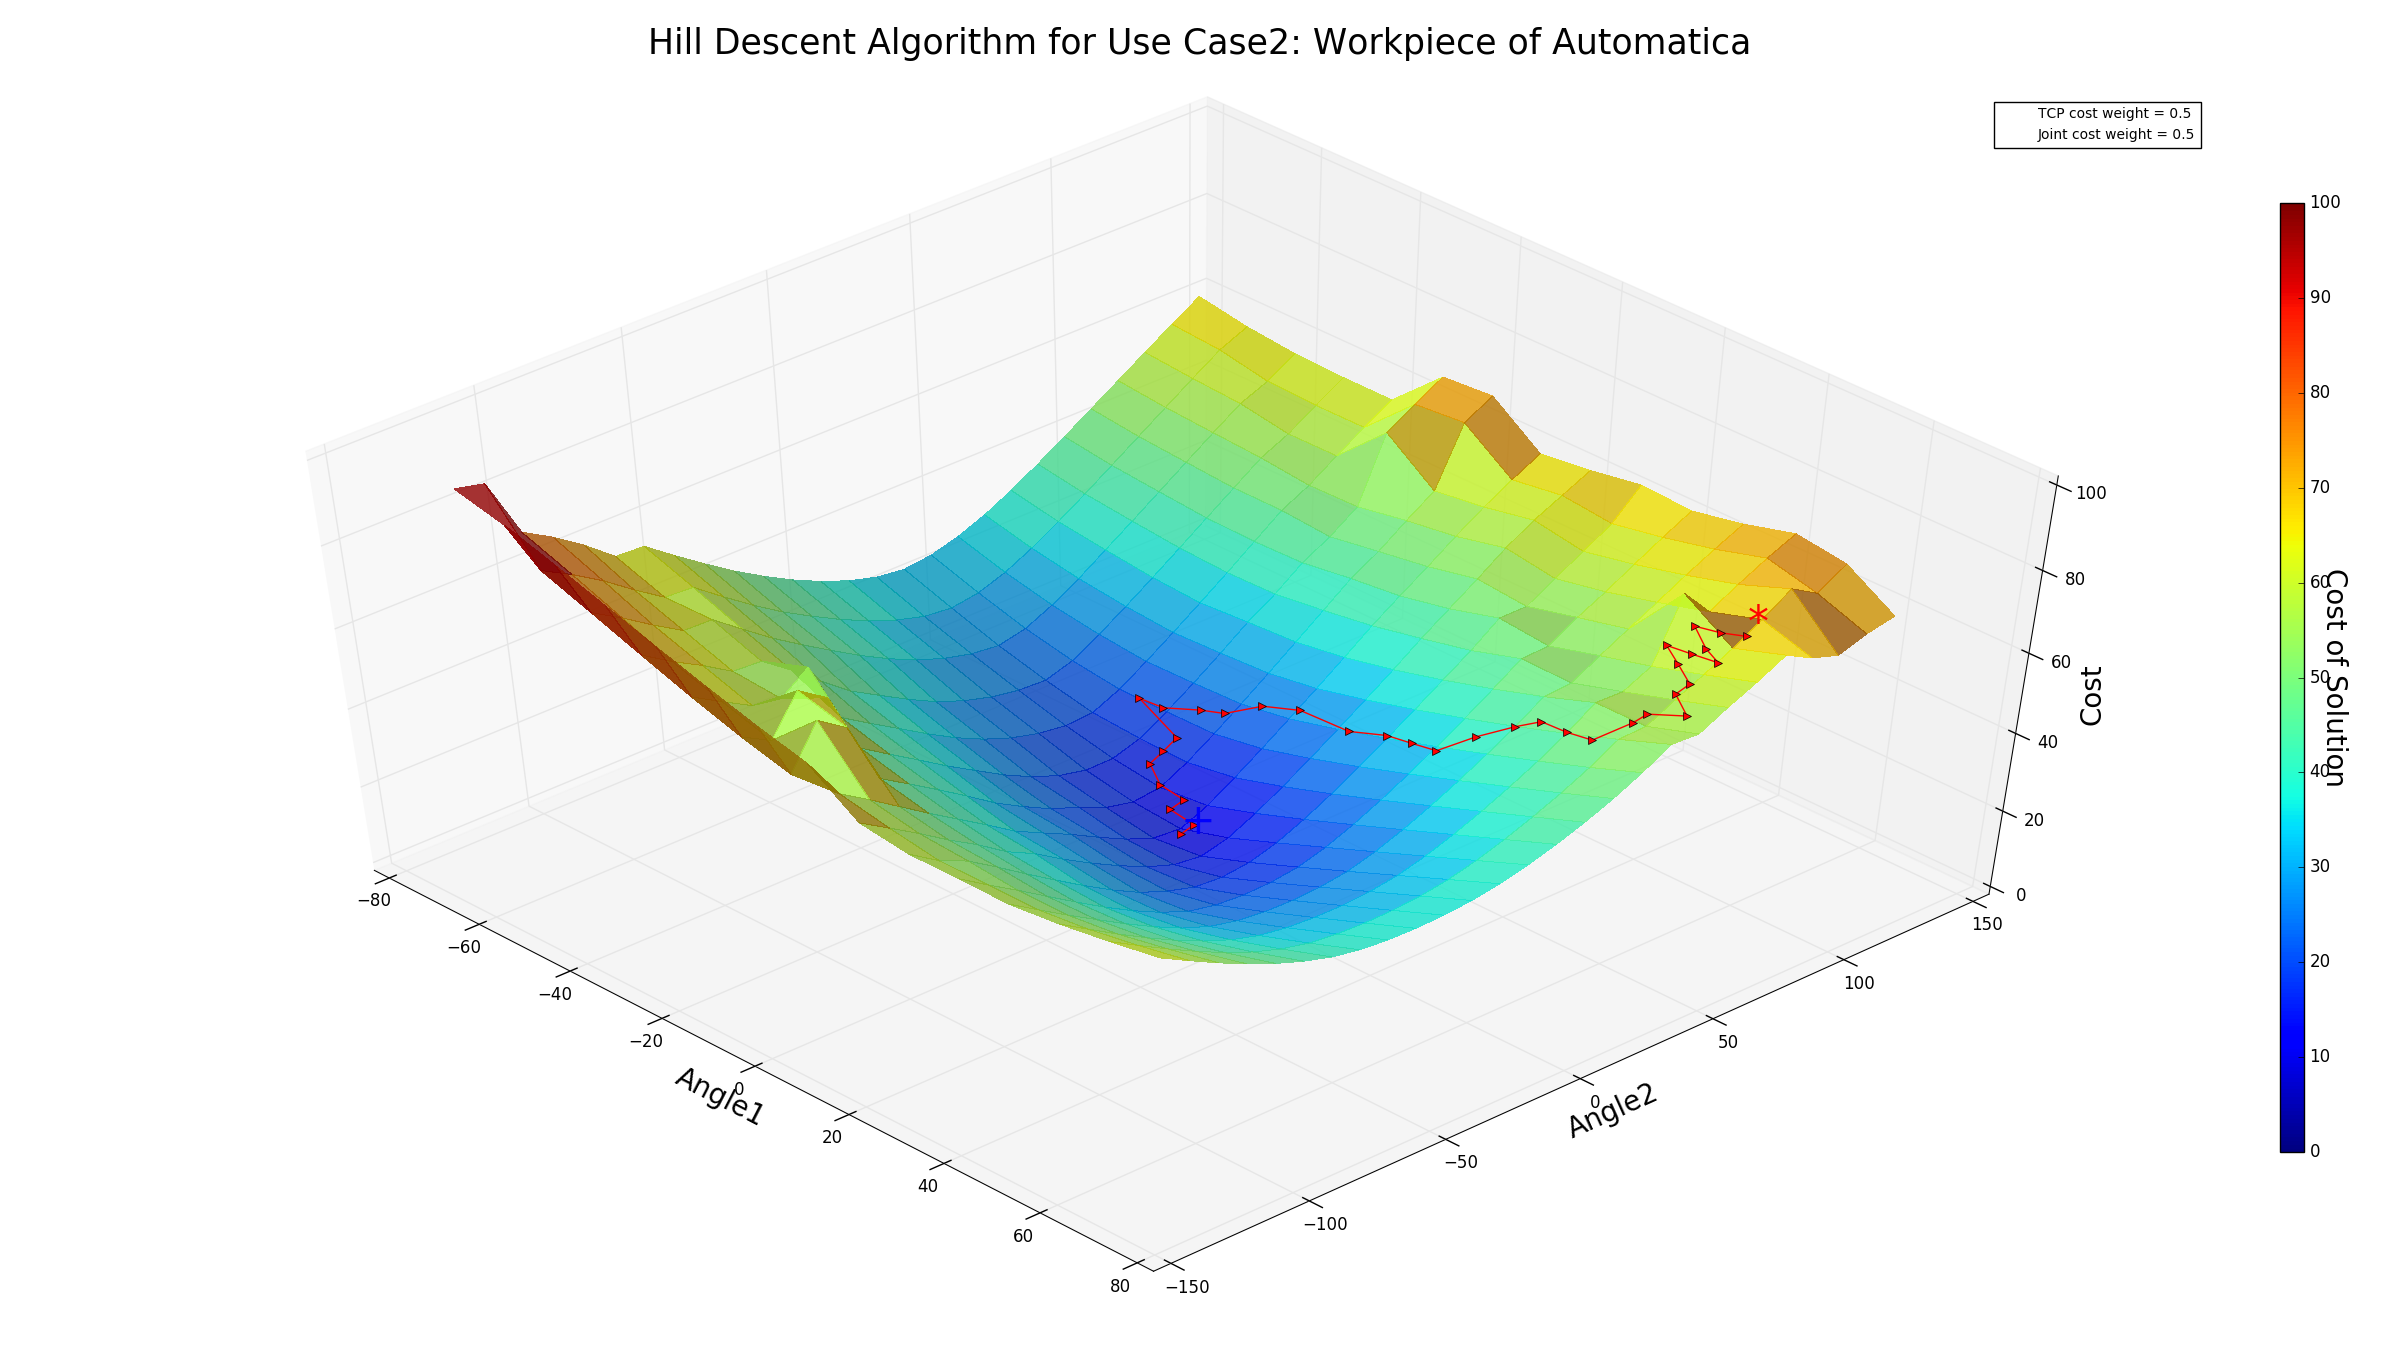
\includegraphics[width=0.8\textwidth,scale=0.6]{images/auto_hori_succ.png}}
	\caption{Hill Descent Optimization for Automatica Workpiece Horizontal Edge(\ref{fig:imguc3})}
	\label{fig:HD1}
\end{figure}
In figure \ref{fig:HD1}, the start state is marked by red star and the goal by blue plus. We can observe that, because the cost surface has a single global minimum, the hill descent approach was able to reach the global minima state.
\begin{figure}[!ht] %  figure placement: here, top, bottom, or page
	\centering
	\frame{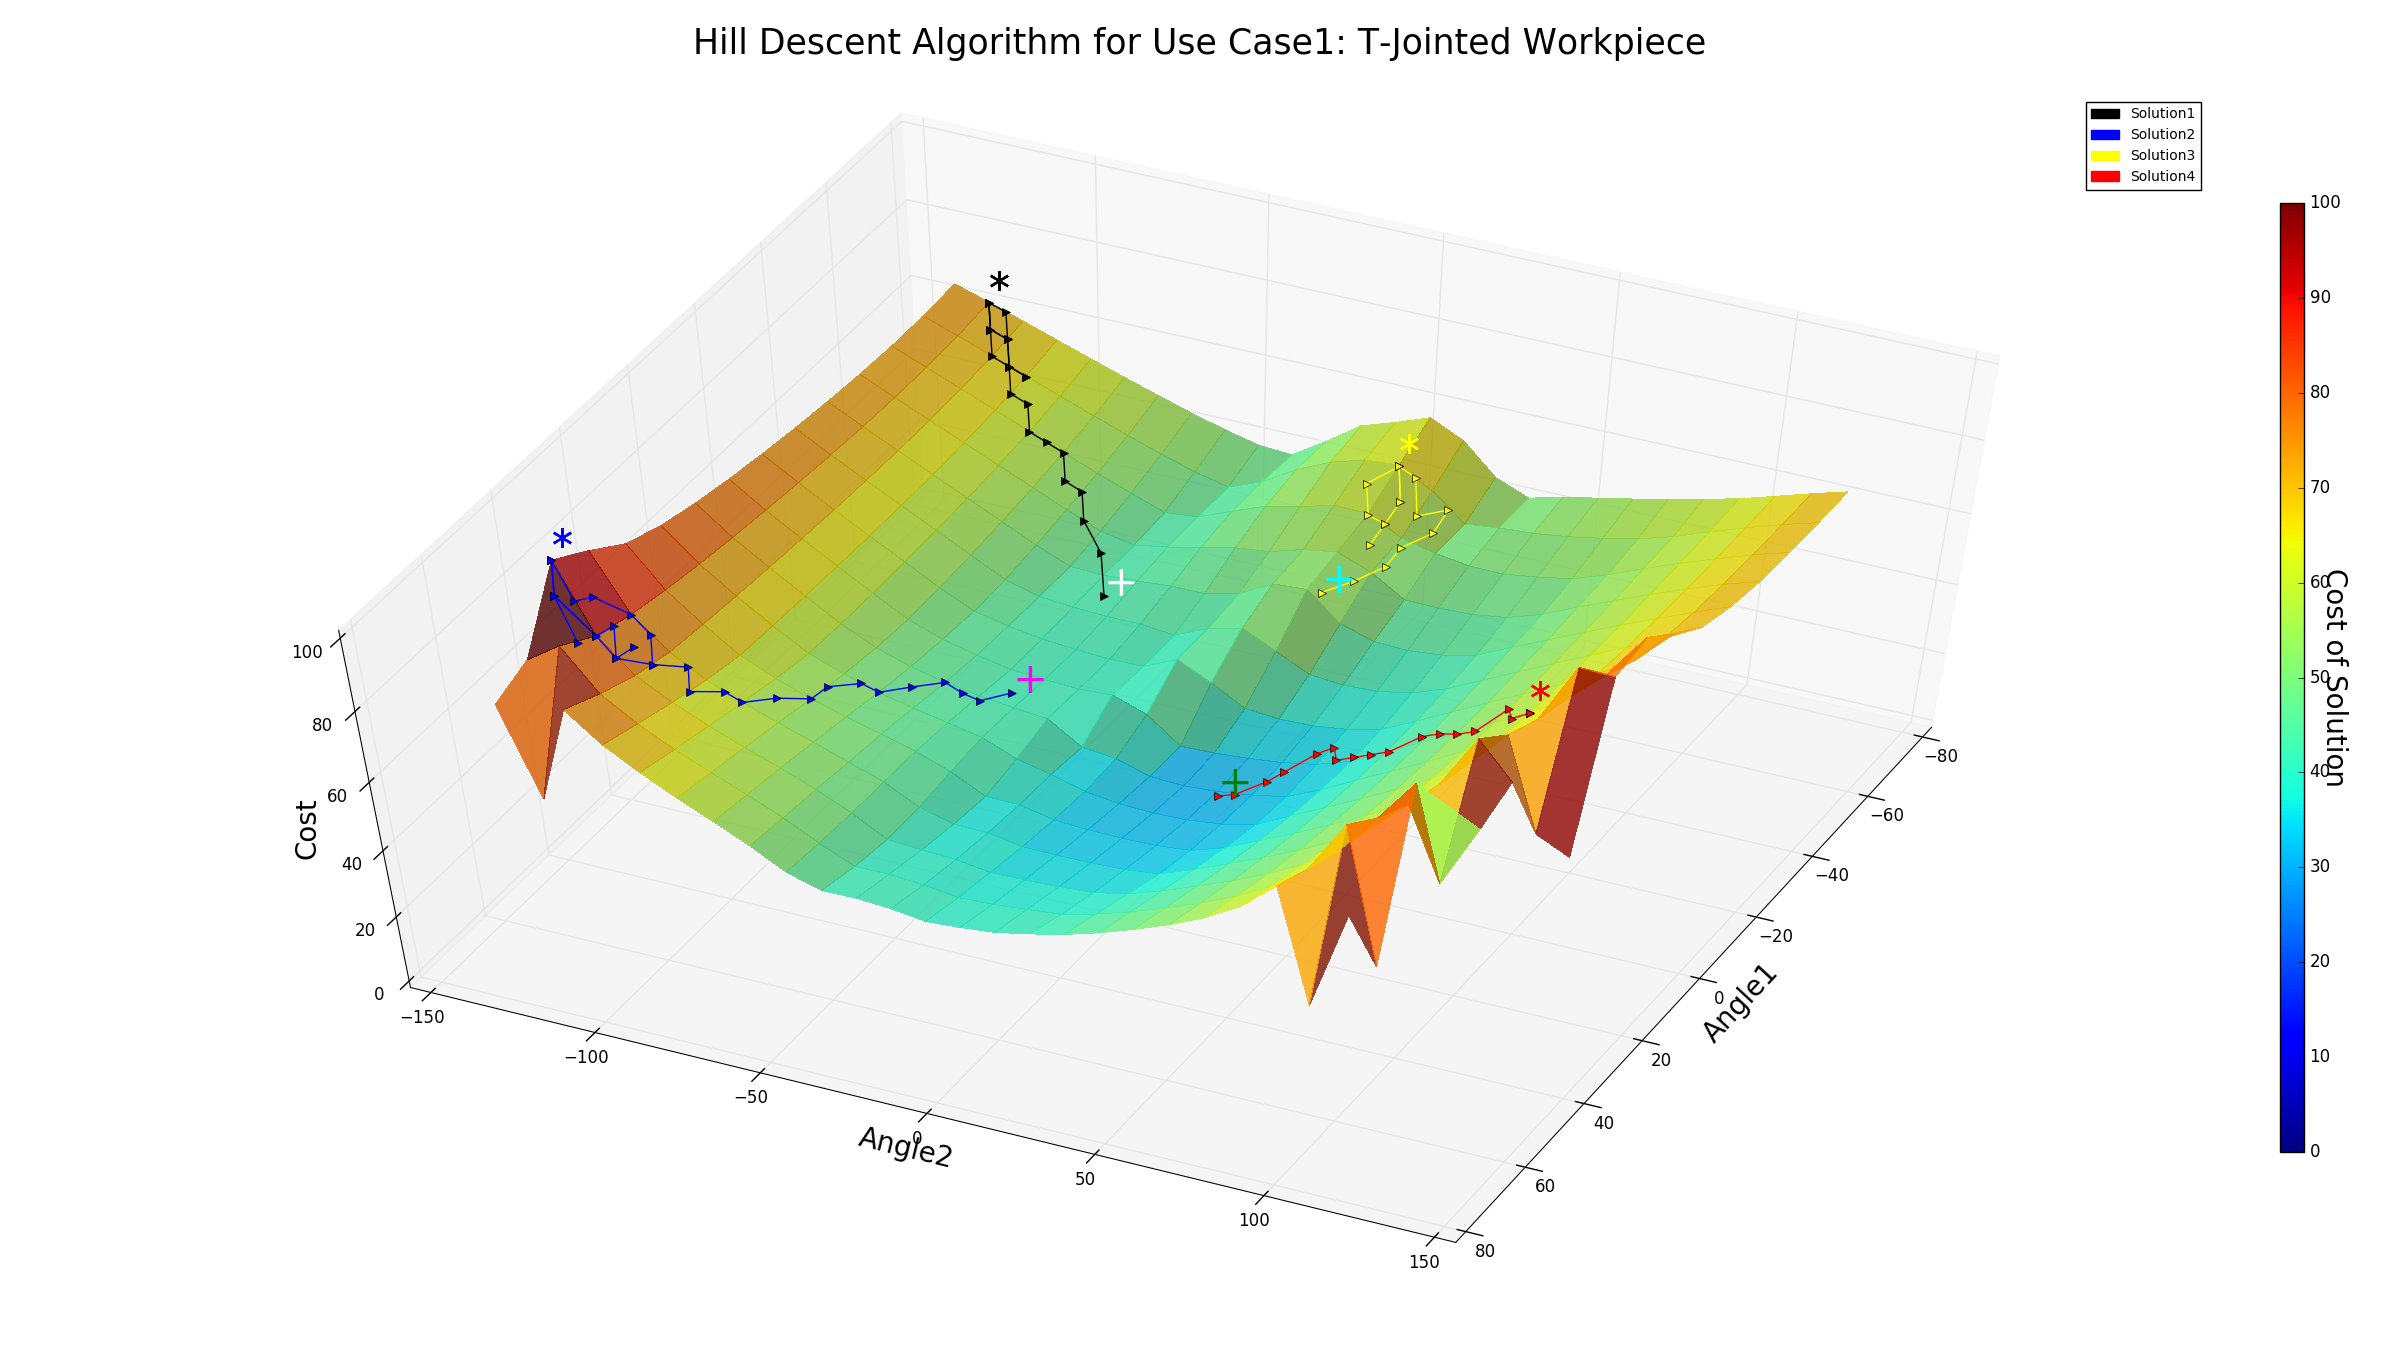
\includegraphics[width=0.8\textwidth,scale=0.6]{images/ori_hill_fail.png}}
	\caption{Hill Descent Optimization for T-Jointed Workpiece Horizontal Edge(\ref{fig:imguc2})}
	\label{fig:HD2}
\end{figure}\\
However, in figure \ref{fig:HD2} we can see that, because the cost surface has multiple local minima, the Hill Descent based approach gets stuck in a local minima for solutions 1, 2 and 3. This is a well known disadvantage of Hill Descent Algorithm, which nullifies its advantages of low memory consumption and speed\footnote{\label{fn1}To be noted: In figure (\ref{fig:HD1}) and (\ref{fig:HD2}) the cost plots are only shown for illustrative purposes, in the actual program, only the final optimized solution is returned.}. 
\subsubsection{Simulated Annealing Algorithm Approach}
\label{sssec:sa}
In \ref{sssechd}, we observed that the Hill Descent Approach fails to find the most optimal solution, if it encounters a local minima. Simulated Annealing is typically used for cases where the search space might contain one or more local minima points along with a global minima. Simulated annealing can escape local minima by accepting moves with higher cost, based on the outcome of a probability function [\citet{vanLaarhoven1987},\citet{russell2009artificial} ]. 
\begin{algorithm}[!ht]
	\caption{Simulated Annealing Based Optimal Weld Path Generation}
	\label{algo5}
	\textbf{Given:} $ \text{Initial table joint angle values \textit{$A1$} \& \textit{$A2$}}$ \\ 
	\textbf{Output:} $ \text{Table joint values for plan path generation with minimum cost}$
	
	\begin{algorithmic}[1]
		\State $\text{Apply kinematic equation \ref{eq22} and set table position using \textit{$A1$} \& \textit{$A2$}}$
		\State $\text{Apply Workpiece Transformation Algorithm(\ref{algo2})}$
		\State $\text{Apply Selected Edge Transformation Algorithm(\ref{algo2})}$
		\State $\text{Perform Motion Planning on the transformed plan path and get \textit{Solution}}$
		\State $\text{\textit{MinimumCost} $\gets$ $C_{agg}$(\textit{Solution}) using equation(\ref{eq25})}$
		\State $\text{(\textit{$A1_{curr}$},\textit{$A2_{curr}$}) $\gets$ (\textit{$A1$}, \textit{$A2$})}$
		\While {[${temperature > \epsilon}$]}
		\State $\text{(\textit{$A1_{new}$},\textit{$A2_{new}$})}$ $\gets$ $\text{\textit{SelectNeighbor}(\textit{$A1_{curr}$},\textit{$A2_{curr}$})}$
		\State $\text{Apply steps \textit{1-4} with (\textit{$A1_{new}$},\textit{$A2_{new}$})}$
		\State $\text{\textit{Stepcost} $\gets$ $C_{agg}$(\textit{Solution}) \ref{eq25}}$
		\State $\text{VisitedStateArray}$ $\gets$ $\textit{$A1_{curr}$},\textit{$A2_{curr}$}$ $\textit{,Stepcost}$ 
		\State $\text{\textit{diff} $\gets$ \textit{Stepcost} - \textit{MinimumCost}}$
		\If {[${diff < 0 } \textit{ or }$ $e^{-1*diff/temperature} >$  $Rand(0,1) $]}
		\State $\text{(\textit{$A1_{curr}$},\textit{$A2_{curr}$}) $\gets$ (\textit{$A1_{new}$}, \textit{$A2_{new}$})}$
		\State $\text{\textit{MinimumCost} $\gets$ \textit{Stepcost}}$
		\EndIf
		\State $\textit{temperature}$ $\gets$ $\textit{temperature*coolingrate}$
		\EndWhile %doWhile{$\textit{PossibleMinimaCounter} < 8$}
		\State $\textit{return} (\textit{$A1_{curr}$},\textit{$A2_{curr}$})$      
	\end{algorithmic}
\end{algorithm}\\
Similar to hill descent approach, simulated annealing accepts any next move which has a lower cost compared to the current one, however unlike hill descent it also accepts a fraction of moves to states with higher solution cost. The probability of accepting moves to states with higher cost is determined by a continuously decreasing temperature parameter. 
The algorithm terminates when the temperature becomes less than an $\epsilon$ value. In algorithm (\ref{algo5}) , the new table joint angles are selected using euclidean distance. The new states are also stored in a data structure to ensure no duplicate neighbors are generated.
\begin{figure}[!ht] %  figure placement: here, top, bottom, or page
	\centering
	\frame{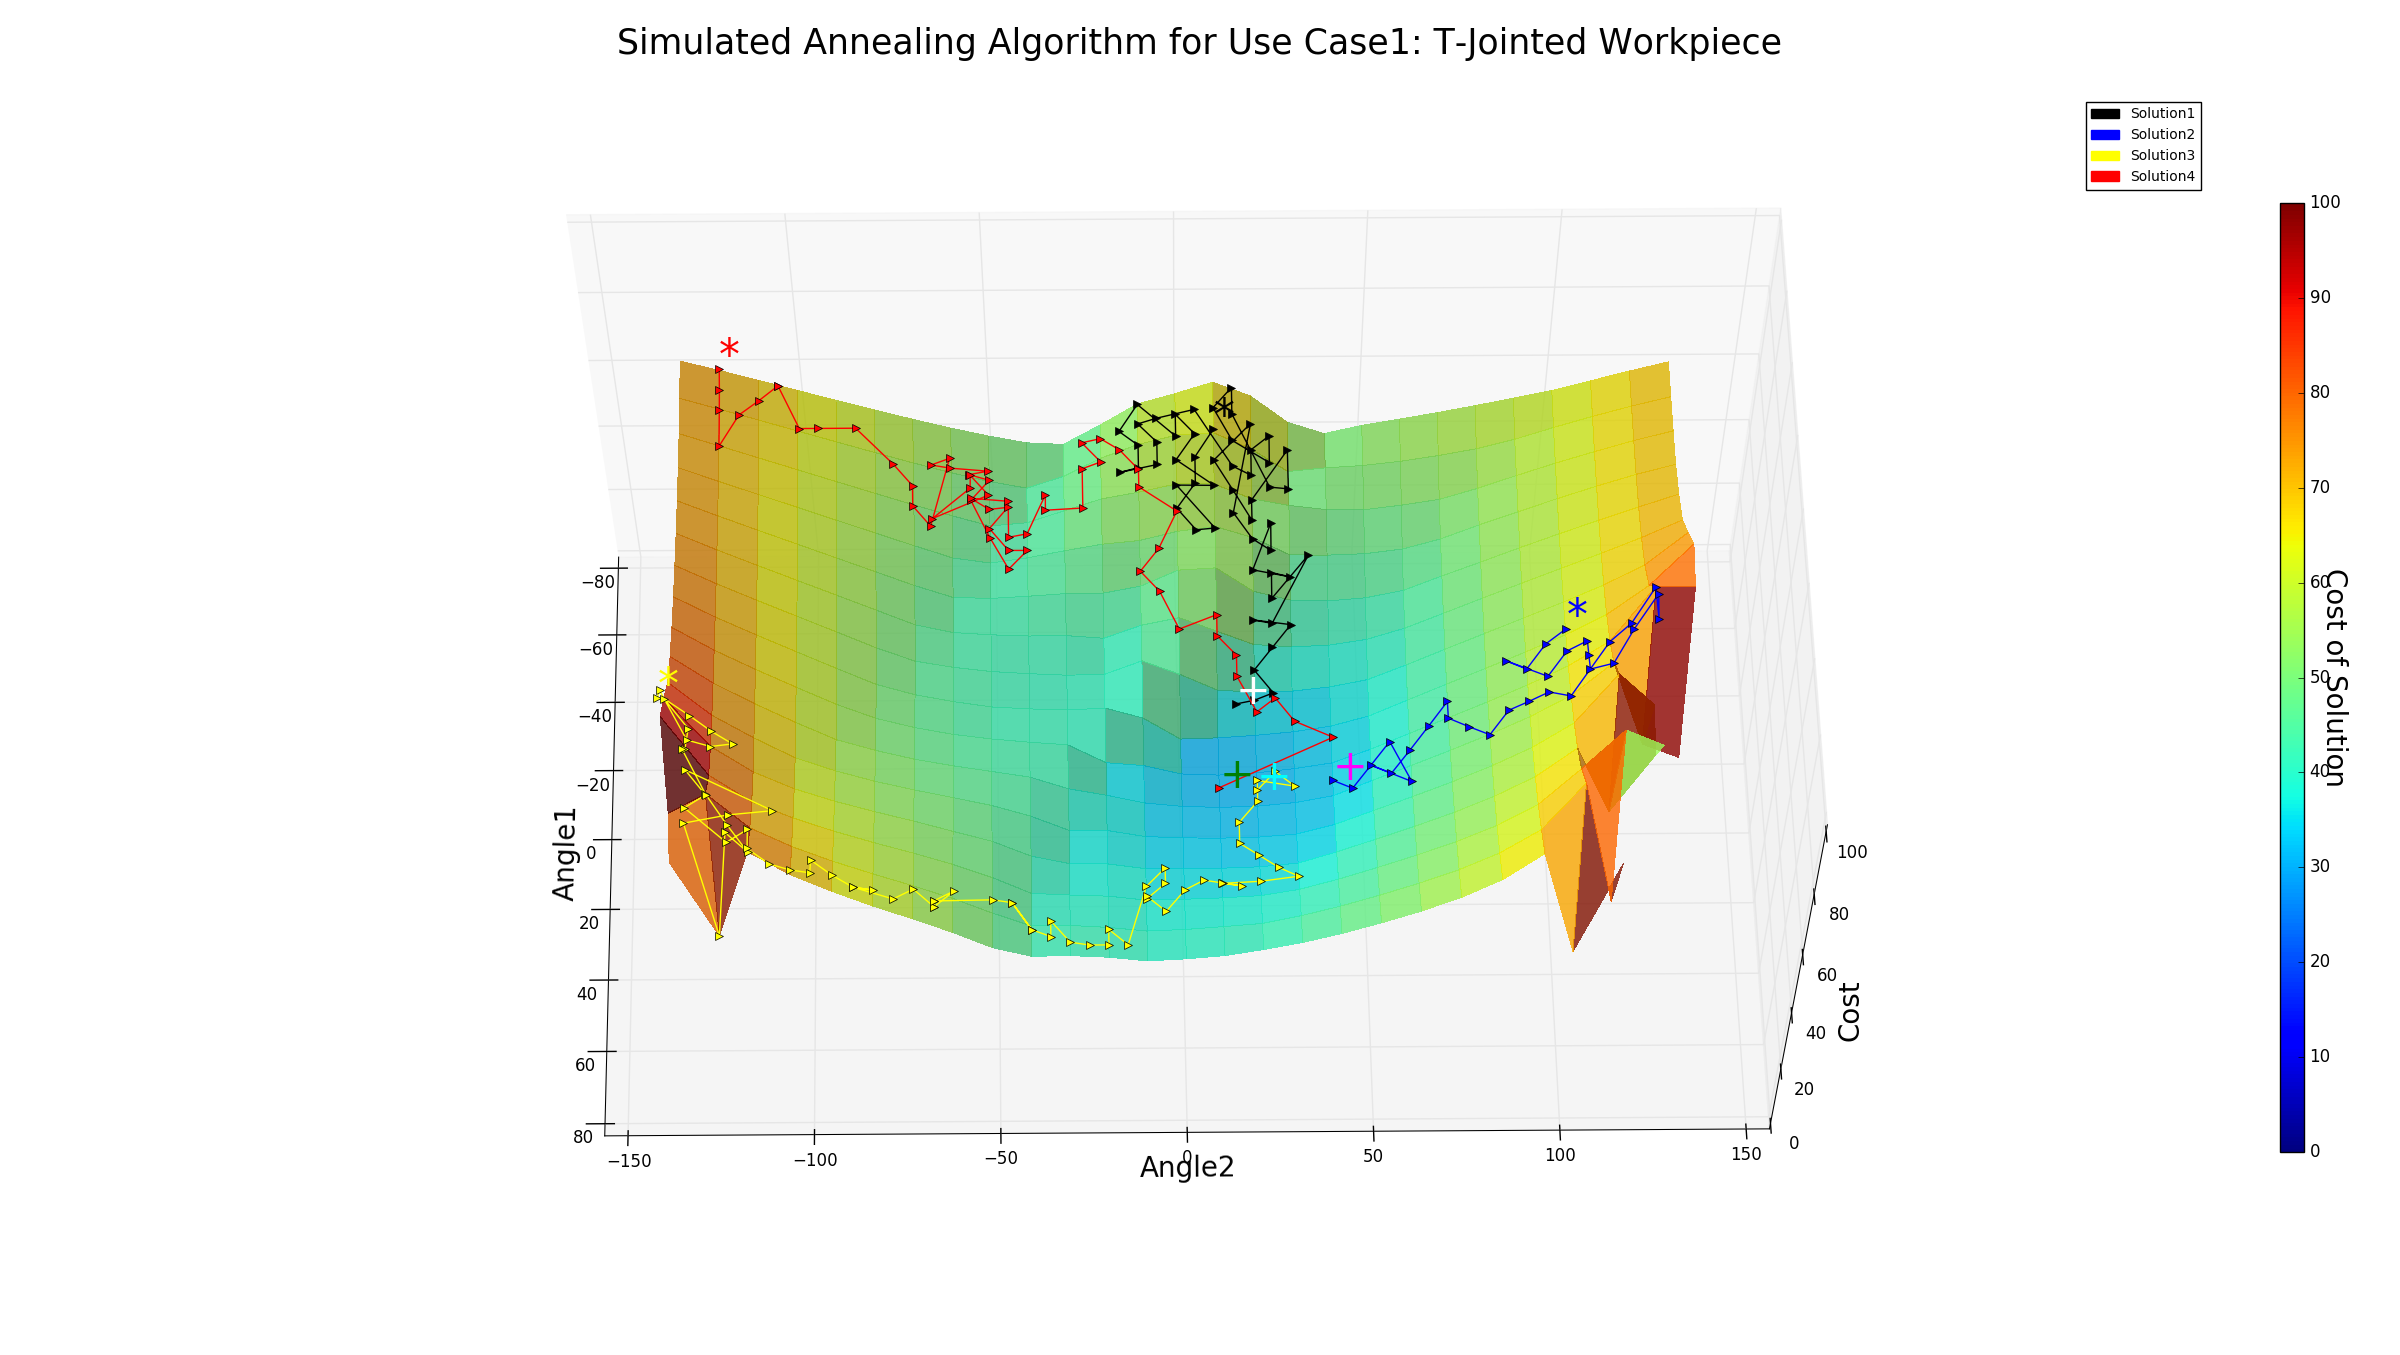
\includegraphics[width=0.8\textwidth,scale=0.6]{images/ori_sa_succ.png}}
	\caption{Simulated Annealing Optimization for T-Jointed Workpiece Horizontal Edge(\ref{fig:imguc2})}
	\label{fig:SA1}
\end{figure}
\begin{figure}[!ht] %  figure placement: here, top, bottom, or page
	\centering
	\frame{\includegraphics[width=0.8\textwidth,scale=0.6]{images/auto_sa_succ.png}}
	\caption{Simulated Annealing Optimization for Automatica Workpiece Horizontal Edge(\ref{fig:imguc3})}
	\label{fig:SA2}
\end{figure}\\
In plot \ref{fig:SA1} and \ref{fig:SA2}, the start and the goal states are  marked by '*' and '+' respectively. We can also observe that unlike the hill descent approach, it was able to find the optimal solution in all cases. However, unlike hill descent approach, in plot (\ref{fig:SA2}) it takes a lot more steps to reach the global minima state even when there are no local minima. 

\paragraph{Random Restart and Termination Condition}
In plot \ref{fig:SA2}, we observed that the simulated annealing algorithm explored a lot of states initially, which delayed the process of finding the global minima. To address this issue we implement a random restart strategy based on the concept mentioned in (\citet{mendivil2001restarting}) to force the algorithm to explore large parts of the cost surface in little time as possible. Also, due to the fact that the global minima is unknown, we implement a termination condition to limit the running of the algorithm. The strategy for the termination condition is based on Optimal Stopping problem method described in (\citet{alizamir2008improving}) . Since randomly starting at different points of the space can cause discrepancy in finding the global minima, we introduce an additional variable - \textit{globalbestcost} - to keep track of the best solution that has been found. 
\subparagraph{Random Restart}
The implementation of random restart based on \citet{mendivil2001restarting} is shown in plot \ref{fig:20}. The random restart points are marked by the arrows. The threshold of random restart was set to 15, i.e. if 15 states with higher cost compared to the current state were found, then it restarted. In the later part, when it came closer to the optimal solution, the newer solutions that were generated were closer to the global minima, hence the solutions converged without performing additional random restarts.
\begin{figure}[!ht] %  figure placement: here, top, bottom, or page
	\centering
	\begin{subfigure}[b]{0.4\textwidth}
	\frame{\includegraphics[width=1\textwidth,height=0.2\textheight]{images/NoRandomRestartSA1.png}}
	\caption{Solution Points Without Random Restart}  
	\label{fig:20a}
	\end{subfigure}	
	\begin{subfigure}[b]{0.4\textwidth}
		\frame{\includegraphics[width=1\textwidth,height=0.2\textheight]{images/RandomRestartSA1.png}}
		\caption{Solution Points With Random Restart}  
		\label{fig:20b}
	\end{subfigure}	
\caption{Plots Showing Effect of Random Restart on number of iterations}
\label{fig:20}
\end{figure}

%\begin{figure}[!ht] %  figure placement: here, top, bottom, or page
%	\centering
%	\frame{\includegraphics[width=0.7\textwidth,scale=0.6]{images/RandomRestartSA.png}}
%	\caption{Random Restart Approach for Simulated Annealing Optimization(Restart point marked with arrows)}
%	\label{fig:RR1}
%\end{figure}
\algnewcommand{\LeftComment}[1]{\Statex \(\triangleright\) #1}
\def\HiLi{\leavevmode\rlap{\hbox to \hsize{\color{yellow!50}\leaders\hrule height .8\baselineskip depth .5ex\hfill}}}
\begin{algorithm}
	\caption{Simulated Annealing Approach for Optimal Weld Path Generation}
	\label{algo6}
	\textbf{Given:} $ \text{Initial table joint angle values \textit{$A1$} \& \textit{$A2$}}$ \\ 
	\textbf{Output:} $ \text{Table joint values for plan path generation with minimum cost}$ 
	
	\begin{algorithmic}[1]
		\State $\text{Apply kinematic equation \ref{eq22} and set table position using \textit{$A1$} \& \textit{$A2$}}$
		\State $\text{Apply Workpiece Transformation Algorithm(\ref{algo2})}$
		\State $\text{Apply Selected Edge Transformation Algorithm(\ref{algo2})}$
		\State $\text{Perform Motion Planning on the transformed plan path and get \textit{Solution}}$
		\State $\text{\textit{MinimumCost} $\gets$ $C_{agg}$(\textit{Solution}) \ref{eq25}}$
		\State \HiLi $\text{\textit{globalbestcost} $\gets$ $C_{agg}$(\textit{Solution}) \ref{eq25}}$
		\State $\text{(\textit{$A1_{curr}$},\textit{$A2_{curr}$}) $\gets$ (\textit{$A1$}, \textit{$A2$})}$
		\While {[${temperature > \epsilon}$]}
		\If {\HiLi[${counter > threshold}$]}                	
		\State \HiLi $\textit{counter}$ $\gets$ $0$ \Comment{do random restart to escape local minima} 
		\State \HiLi $\text{(\textit{$A1_{new}$},\textit{$A2_{new}$})}$ $\gets$ $\text{\textit{RandomNeighbor}}$
		\Else
		\State $\text{(\textit{$A1_{new}$},\textit{$A2_{new}$})}$ $\gets$ $\text{\textit{SelectNeighbor}(\textit{$A1_{curr}$},\textit{$A2_{curr}$})}$
		\EndIf
		\State $\text{Apply steps \textit{1-4} with (\textit{$A1_{new}$},\textit{$A2_{new}$})}$
		\State $\text{\textit{Stepcost} $\gets$ $C_{agg}$(\textit{Solution}) \ref{eq25}}$
		\State $\text{VisitedStateArray}$ $\gets$ $\textit{$A1_{curr}$},\textit{$A2_{curr}$}$ $\textit{,Stepcost}$ 
		\State $\text{\textit{diff} $\gets$ \textit{Stepcost} - \textit{MinimumCost}}$
		\If {\HiLi[${\textit{Stepcost} < \textit{globalbestcost}}$]}
		\State \HiLi $\textit{globalbestcost}$ $\gets$ $\textit{Stepcost}$
		\EndIf
		\If {[${diff < 0 } \textit{ or }$ $e^{-1*diff/temperature} >$  $Rand(0,1) $]}
		\State $\text{(\textit{$A1_{curr}$},\textit{$A2_{curr}$}) $\gets$ (\textit{$A1_{new}$}, \textit{$A2_{new}$})}$
		\State $\text{\textit{MinimumCost} $\gets$ \textit{Stepcost}}$
		\EndIf
		\If {\HiLi[${diff > 0 }$]}
		\State \HiLi $\text{increase }$ $\textit{ counter }$ $\text{ by 1}$
		\EndIf
		\State $\textit{temperature}$ $\gets$ $\textit{temperature*coolingrate}$
		\EndWhile 
		\State $\textit{return} (\textit{$A1_{curr}$},\textit{$A2_{curr}$})$      
	\end{algorithmic}
\end{algorithm}
Algorithm (\ref{algo6}) details the steps for the random restart procedure implemented based on the approach mentioned in (\citet{mendivil2001restarting}). The additional steps which were inducted to the Simulated Annealing Algorithm (\ref{algo5}) are highlighted with yellow. 
\subparagraph{Termination Condition}
Theoretically, if simulated annealing algorithm is allowed to run for infinite time it is always guaranteed to find the most optimal solution, in other words it can be termed as asymptotically optimal. However ,such method is not only impractical, but also computationally expensive. In each iteration the algorithm has to search through the list of existing neighbors, whose size increases at each step - as new neighbors are added -, thus making the search take up longer time. Simulated Annealing usually finds the global minima in finite steps, thus having a termination condition will not affect the quality of solution rather it will improve the algorithm run time. Based on (\citet{alizamir2008improving}), we formulate the following termination criteria:
\begin{itemize}
	\item As normally with simulated algorithm, at each step, compare the current cost with previous state cost.
	\item If the cost of current state is lesser than the previous state cost, calculate the \textit{improvementpercentage} i.e (cost of previous state - cost of current step)$/$cost of previous state.
	\item The complexity of checking for already existing state is given by \textit{O($n^{2}$)}, this can be explained by the fact that we need two nested for loops to perform this check. 
	\item Calculate the \textit{incrementpercentage} i.e: (cost for searching through n+1 states of \textit{VisitedStateArray} - cost for searching through n states of \textit{VisitedStateArray})/cost for searching through n states of \textit{VisitedStateArray}.
	\item At each step we calculate the ratio of \textit{improvementpercentage} and \textit{incrementpercentage} and it its lower than an $\epsilon$ value then terminate algorithm
	\item The idea behind this termination definition is, if for every additional step the algorithm takes, if the reward of getting an improved solution is very low compared to the cost of searching through \textit{VisitedStateArray}, then the algorithm has reached the optimal value.
	\item The exit criteria will not be triggered in the initial stages of simulated annealing, as the size of \textit{VisitedStateArray} is quite low, however when the size of \textit{VisitedStateArray} becomes quite large, due to the $n1^{2}$ factor, the ratio will be low and the algorithm will terminate
\end{itemize}

\subsection{Comparative Evaluation and Analysis}
The most important aspects of Simulated Annealing algorithm, which determine its performance are the 'Cooling Schedule' and 'Cooling Rate'. In (\citet{nourani1998comparison}), the authors discusses the various cooling schedules applicable for simulated annealing. In table \ref{tab:table1}, we present the data recorded during our run of Simulated Annealing for use case (\ref{fig:imguc2}) with starting angle at (50,-130). We recorded the time of completion, number of iterations and memory consumed by the storage data structure storing all the visited neighbors. All the tests were carried out on a PC with core i7 processor and 8 Giga Bytes of memory. 

\begin{table}[!ht]
	\centering
	\resizebox{\textwidth}{!}{%
	\begin{tabular}{@{}ccccll@{}}
		\toprule
		& \textbf{Time(secs)} & \textbf{\begin{tabular}[c]{@{}c@{}}Number of \\ Iterations\end{tabular}} & \textbf{\begin{tabular}[c]{@{}c@{}}Memory Consumed\\ (Bytes)\end{tabular}} & \textbf{Status} & \textbf{Solution} \\ \midrule
		\textbf{\begin{tabular}[c]{@{}c@{}}Exponential \\ Multiplicative\\ Cooling\end{tabular}}    & 450.22              & 168                                                                      & 4032                                                                       & Complete        & Optimal           \\
		\textbf{\begin{tabular}[c]{@{}c@{}}Logarithmic \\ Multiplicative\\  Cooling\end{tabular}} & 389.6              & 119                                                                      & 2856                                                                       & Complete        & Sub-Optimal           \\
		\textbf{\begin{tabular}[c]{@{}c@{}}Linear\\ Multiplicative\\ Cooling\end{tabular}}          & 3746.11             & 293                                                                      & 7032                                                                       & Complete        & Optimal           \\
		\textbf{\begin{tabular}[c]{@{}c@{}}Quadratic\\ Multiplicative\\ Cooling\end{tabular}}       & 373.01              & 34                                                                       & 816                                                                        & Complete        & Sub-optimal       \\ \bottomrule
	\end{tabular}
	
}
\caption{Simulated Annealing Cooling Schedules}
\label{tab:table1}
\end{table}

\begin{figure}[!ht] %  figure placement: here, top, bottom, or page
	\centering
	\frame{\includegraphics[width=0.8\textwidth,scale=0.6]{images/cooling_schedules.png}}
	\caption{Simulated Annealing Cooling Schedules}
	\label{fig:CS}
\end{figure}

From the data above we can observe for Exponential Multiplicative Cooling, we reach the optimal solution in a reasonable time, while consuming a descent amount of memory. Next we will present the data for different cooling rates for Exponential Multiplicative Cooling on the same solution set, starting from (-50,130).

\begin{table}[!ht]
	\centering
	\resizebox{\textwidth}{!}{%
	\begin{tabular}{@{}ccccll@{}}
		\toprule
		Cooling Rate  & \textbf{Time(secs)} & \textbf{\begin{tabular}[c]{@{}c@{}}Number of \\ Iterations\end{tabular}} & \textbf{\begin{tabular}[c]{@{}c@{}}Memory Consumed\\ (Bytes)\end{tabular}} & \textbf{Status} & \textbf{Solution} \\ \midrule
		\textbf{0.95} & 598.37              & 171                                                                      & 4104                                                                       & Complete        & Optimal           \\
		\textbf{0.9}  & 328.88              & 65                                                                       & 1560                                                                       & Complete        & Optimal           \\
		\textbf{0.85} & 185.45              & 43                                                                       & 1032                                                                       & Incomplete      & Sub-optimal       \\
		\textbf{0.8}  & 132.50              & 29                                                                       & 696                                                                        & Incomplete      & Sub-optimal       \\ \bottomrule
	\end{tabular}
	
}
\caption{Simulated Annealing Cooling Rates for Exponential Multiplicative Cooling}
\label{table2}
\end{table}

From table \ref{table2} we can observe that 0.9 is the most optimal cooling rate that can be chosen, which converges to an optimal solution, while consuming a descent amount of memory. 

\begin{figure}[!ht] %  figure placement: here, top, bottom, or page
	\centering
	\frame{\includegraphics[width=0.8\textwidth,scale=0.6]{images/cooling_rates.png}}
	\caption{Simulated Annealing Cooling Rates}
	\label{fig:CR}
\end{figure}









\newpage
\section{Reachability Avoidance}
According to (\citet{craig2005introduction}) a necessary condition for a solution to exist, is to verify whether it exists in the workspace of the manipulator. Workspace is defined as the end effector's reachable volume(\citet{craig2005introduction}). Therefore it goes without saying that to ensure that the generated weld paths are valid, we have to ensure that they are free from unreachable points. In the existing system[\citet{DiazP2016}] the robot could only check whether a point lay in the reachable workspace or not, but there was no method to avoid it or generate an alternate path. The only solution was to manually move the work piece to a position, where unreachable points were not present. Manually moving the workpiece created the following problems:
\begin{itemize}
	\item After moving the workpiece, it was necessary to remeasure its position coordinates and enter the new values to the software. Often re measurement was required to ensure that the workpiece has been placed in the proper position.
	\item If more than one edge of a workpiece was needed to welded, and one of the edges fell in a non-reachable position, moving the workpiece and trying to recalibrate its position proved to be an extremely tedious and inefficient method. Often this resulted in abandoning the generated plan and starting anew.
	\item Placing the workpiece in a fixed position on the table every time, provided a sub-optima solution. However this meant that it was necessary to mark positions for each and every workpiece and accurately set them up each and every time they were to be welded.	
\end{itemize} 

Using the 2Dof rotary table to solve the problem of reachability provided the following advantages:
\begin{itemize}
	\item The table can be moved multiple times and each and every time we will know the precise position of the workpiece using algorithm (\ref{algo2}).
	\item Since we also calculate the new position of the weld path, when the table is rotated,(using algorithm (\ref{algo3}) ), hence we can generate weld paths for different edges, without manually altering the workpiece position.
	\item Constraint on placing the workpiece at a fixed position is removed, thus providing greater flexibility to the welding process.
\end{itemize}
\subsection{Reachability and Motion Planning}
In (ppr paper), an inverse kinematic based approach for detecting whether a point is unreachable or not is implemented. It takes the Cartesian coordinates of a point and computes the Inverse Kinematics to get the joint values. If the solution generated is valid, then the point is flagged as reachable, otherwise it is marked as unreachable. In order to generate valid plan paths with the motion planner, it was necessary to link the reachability checker with the planning algorithm. 
The steps for detecting unreachable points with the motion planner are described below:
\begin{itemize}
	\item After the path to be weld has been defined, the start and goal points of the selected edge are used to create the OMPL space, using the methodology described in (ppr).
	\item The planner(in our case RRTstar) is configured and planning is started.
	\item OMPL uses a state validity checker class to check whether a generated sample is valid or not. The definition of validity can be set by the user. In our case we link the reachability detection algorithm with the validity checker.
	\item The planner returns a true or false value based on whether a point is reachable or not.
	\item If all the planner is successfully able to connect the start and goal points without having any invalid points in between, the solution is marked as successful and the cumulative cost value of the path is calculated using equation(\ref{eq25}).
	\item If however the planner fails to find a valid solution, we assign a very high cost value to the failed solution. 
\end{itemize} 

\subsection{Use Case Description}
\label{ssec:usc1}
We present a use case, figure(\ref{fig:rc1}), the  workpiece edge to be welded is marked with yellow. We generate the following plots \ref{fig:rc1} and \ref{fig:rc2} for visualizing the cost surface and the reachable planned paths for
 the manipulator with respect to the movement of the workpiece.
\begin{figure}[!ht] %  figure placement: here, top, bottom, or page
	\centering
	\frame{\includegraphics[width=0.8\textwidth,scale=0.6]{images/Urchbl_uscs.png}}
	\caption{Unreachable Use Case}
	\label{fig:rc1}
\end{figure} 
When an

\begin{figure}[!ht] %  figure placement: here, top, bottom, or page
	\centering
	\frame{\includegraphics[width=0.8\textwidth,scale=0.6]{images/Rchbl_cst1.png}}
	\caption{Cost Space Plot}
	\label{fig:rc2}
\end{figure}

In figure \ref{fig:rc2}, the part marked with the deepest red color has the highest cost, i.e. weld paths generated for those joint angles of the table are unreachable. When joint angle 2 value either reaches $-180^{circle}$ or $+180^{circle}$ the cost value reaches its minimum. This can be explained by the fact that when joint angle 2 of the table rotates to either values, the selected workpiece edge faces the robot, thereby decreasing joint angle movement required by the manipulator for tracing the planned path. Facing the workpiece edge towards the manipulator also allows the tool tip orientation to follow the optimal orientation definition. 

A map for the reachable workspace of the manipulator, based on the table movement is presented in figure . Here we plot all the reachable weld plan path points. The points marked in magenta are unreachable, while the blue ones are reachable. 
\begin{figure}[!ht] %  figure placement: here, top, bottom, or page
	\centering
	\frame{\includegraphics[width=0.8\textwidth,scale=0.6]{images/Rchbl_spc5.png}}
	\caption{Reachability Space Map}
	\label{fig:rc3}
\end{figure}

\subsection{Implementation and Results}
In the previous section \ref{ssec:usc1} we formulated the problem of unreachability into a cost function, in which the unreachable states were assigned high costs. Next, we use the approach described in section \ref{sssec:sa} in order to not only reposition the workpiece into a reachable position relative to the manipulator, but also ensure that it is in the most optimal position. The plot for the solution on the cost surface is illustrated in figure \ref{fig:rc4}. The start point is marked by the green '*' and the goal is marked by '+' sign. From the plot we can clearly observe that the algorithm reaches the global minima. 
\begin{figure}[!ht] %  figure placement: here, top, bottom, or page
	\centering
	\frame{\includegraphics[width=0.8\textwidth,scale=0.6]{images/Rchbl_cst_sln.png}}
	\caption{Cost Plot of Reachability and Solution }
	\label{fig:rc4}
\end{figure}
The solution in RobotKit is shown in figure \ref{fig:rc5}.
\begin{figure}[!ht] %  figure placement: here, top, bottom, or page
	\centering
	\frame{\includegraphics[width=0.8\textwidth,scale=0.6]{images/Urchbl_uscs_slv.png}}
	\caption{Cost Plot of Reachability and Solution }
	\label{fig:rc5}
\end{figure}
\clearpage



\newpage
\section{Benchmarking of Planners}
In the previous sections, we found out the path plans for optimal welding using the 2Dof rotary table. We also addressed the problem of reachability and showed how it can be overcome using the table. In this chapter we will delve into the effects that the table has on the motion planners, in terms of time taken to generate a plan, correctness of solution generated and memory consumed while doing so. We consider 2 different scenarios, for benchmarking the planners first without optimizing the table position and next with the table optimization turned on. The results show a remarkable improvement, in terms of both time and valid solution generation when table optimization is used. The use cases are illustrated in figures (\ref{bm:uc1} and \ref{bm:uc2}).
The configuration details of the planners are presented in the appendix section.
\begin{figure}[!htbp] %  figure placement: here, top, bottom, or page
	\centering
	\begin{subfigure}[b]{0.4\textwidth}
		\frame{\includegraphics[width=1\textwidth,height=0.2\textheight]{images/un_opt_bnch.png}}
		\caption{Use Case Without Table Position Optimization}  
		\label{bm:uc1}
	\end{subfigure}
	\begin{subfigure}[b]{0.4\textwidth}
		\frame{\includegraphics[width=1\textwidth,height=0.2\textheight]{images/opt_bnch.png}}
		\caption{Use Case With Table Position Optimization}  
		\label{bm:uc2}
	\end{subfigure}	
	\caption{Benchmarking Use Cases}
	\label{bm:uc}
\end{figure}

\begin{figure}[!ht] %  figure placement: here, top, bottom, or page
	\centering
	\frame{\includegraphics[width=0.8\textwidth,scale=0.6]{images/norm_time-1.png}}
	\caption{Time Consumed for Unoptimized Motion Planning }
	\label{fig:bm1}
\end{figure}
\begin{figure}[!ht] %  figure placement: here, top, bottom, or page
	\centering
	\frame{\includegraphics[width=0.8\textwidth,scale=0.6]{images/opt_time-1.png}}
	\caption{Time Consumed for Optimized Motion Planning with Table}
	\label{fig:bm2}
\end{figure}
\begin{figure}[!ht] %  figure placement: here, top, bottom, or page
	\centering
	\frame{\includegraphics[width=0.8\textwidth,scale=0.6]{images/norm_status-1.png}}
	\caption{Status of Motion Planning: Unoptimized}
	\label{fig:bm3}
\end{figure}
\begin{figure}[!ht] %  figure placement: here, top, bottom, or page
	\centering
	\frame{\includegraphics[width=0.8\textwidth,scale=0.6]{images/opt_status-1.png}}
	\caption{Status of Motion Planning:Using Table Optimization}
	\label{fig:bm4}
\end{figure}
\begin{figure}[!ht] %  figure placement: here, top, bottom, or page
	\centering
	\frame{\includegraphics[width=0.8\textwidth,scale=0.6]{images/norm_memory-1.png}}
	\caption{Memory Consumption of Planners without Table Optimization}
	\label{fig:bm5}
\end{figure}
\begin{figure}[!ht] %  figure placement: here, top, bottom, or page
	\centering
	\frame{\includegraphics[width=0.8\textwidth,scale=0.6]{images/opt_memory-1.png}}
	\caption{Memory Consumption of Planners with Table Optimization }
	\label{fig:bm6}
\end{figure}
\begin{figure}[!ht] %  figure placement: here, top, bottom, or page
	\centering
	\frame{\includegraphics[width=0.8\textwidth,scale=0.6]{images/norm_corrsol-1.png}}
	\caption{Number of Correct Solutions Generated without Table Optimization}
	\label{fig:bm7}
\end{figure}
\begin{figure}[!ht] %  figure placement: here, top, bottom, or page
	\centering
	\frame{\includegraphics[width=0.8\textwidth,scale=0.6]{images/opt_corrsol-1.png}}
	\caption{Number of Correct Solutions Generated With Table Optimization}
	\label{fig:bm8}
\end{figure}
From the results its clear, the table optimization works.
\newpage
\section{Future Works}
\newpage
\input{Chapter8}
%\newpage
\section{Conclusion}
\localtableofcontents
The main purpose of this thesis work was to improve upon the existing autonomous welding process mainly used in SMEs(Small and Medium Scale Industries). Some of the assumptions made in the state of the art systems are:
\begin{itemize}
	\item The work piece edge to be welded always lies in the reachable workspace of the robot. 
	\item The work piece edge will always align with the optimal weld angle definition.
\end{itemize}
Since the robot position is fixed inside the welding cell, the 2Dof rotary table was used to manipulate the work piece, which subsequently increased the degrees of freedom of the whole system (manipulator + rotary table). The major contributions and possible improvements are highlighted below 
\subsection{Contributions}
\begin{itemize}
	\item \textbf{Creation of CAD models for the table}: Simulating the generated welding path plans is essential, as it allows the user to not only verify its quality, but also ensure that any anomalies or fault that may have occurred in the program doesn't get executed on the robot and cause accidents. Having accurate CAD models help to alleviate these problems by providing accurate simulations. 
	\item \textbf{Kinematic Modeling of the Table}: In order to accurately simulate the behavior of the table, modeling the kinematics was essential. 
	\item \textbf{Cost Function Definitions}: Two cost functions were formulated. (i) Difference of the optimal weld TCP orientation and the actual TCP orientation, modeled the weld quality as a cost function, which allowed us to generate plan paths for better quality welds. (ii) Minimization of the bigger joints movement, allowed us to optimize the power consumption during a welding process.
	\item \textbf{Cost Function Optimization}: Hill Descent and Simulated Annealing based approaches were proposed for finding the optimal states of the defined cost functions. Further analysis revealed, the superiority of the Simulated Annealing based approach.
	\item \textbf{Parameters for Simulated Annealing Based Approach}: Since the process parameters for simulated annealing algorithm - cooling rate, cooling schedules - are specific for the problem being solved, a detailed analysis was carried out to determine the cooling schedule and cooling rate most suited to our problem definition.
	\item  \textbf{Unreachability}: Complete and partial unreachability are one of the major causes why a weld path generation can fail. In this work, we modeled the reachability problem and incorporated it with our cost function definition. Then we used the same Simulated Annealing based approach to solve it.
	\item \textbf{Finding a suitable Planner}: Finally a benchmarking among various planners and subsequent analysis were carried out to determine the most suitable planner for our problem.
\end{itemize}
\subsection{Future Work}
The following key research areas for future work were identified:
\begin{itemize}
	\item Further welding parameters can be studied to model new cost functions. 
	\item \textbf{Unreachability avoidance}: We consider a brute approach to solving the problem of unreachability, by moving the workpiece to a completely different position. Further research can be focused on classifying, whether a plan path is completely or partially unreachable and transforming the workpiece accordingly.
	\item Currently, visual inspection for weld quality evaluation is non existent. Combining, both visual inspection of weld quality and process parameter based weld quality evaluation can be combined to create a robust evaluation architecture.
	\item A database of weld seams, along with their respective definition of optimality can be created (similar to grasp library), which will enable us to generate weld plans even faster. 
\end{itemize}

\newpage
%%try
\section{Future work}
One of the immediate furue works would be implementation and evaluation of the proposed architecture on a real ro
%\newpage
% create bibtex document
%\bibliographystyle{alpha} % mit Buchstaben
%\bibliographystyle{plain} % normal
\bibliographystyle{unsrt} % in reinfolge des Textes
%\bibliographystyle{abbrv} % wie plan , nur abgek�rtz
%\bibliographystyle{ieeetr}
%\bibliographystyle{unsrtnat}

\bibliography{BibTex}


\end{document}


